
\documentclass[english,a4paper]{article}



\usepackage{ifdraft}
\usepackage{pgf}
\usepackage{xspace}


\usepackage[english]{babel}
\usepackage{geometry}
\usepackage{makeidx}
\usepackage{tabto}
\usepackage{fancyhdr}
\usepackage{multicol}


\usepackage{marvosym}
\usepackage{amsfonts}
\usepackage{amssymb}
\usepackage{stmaryrd}
\usepackage{braket}
\usepackage{bbold}
\usepackage{bbm}

\usepackage{braket}
\usepackage{extarrows}
\usepackage{colonequals}


\usepackage{mathtools}
\usepackage{amsmath}
\usepackage{amsthm}
\usepackage{cases}
\usepackage{multirow, bigdelim}
\usepackage{nicefrac}
\usepackage{relsize}


\usepackage{algorithm}
\usepackage{algorithmic}


\usepackage{array}
\usepackage{enumerate}
\usepackage[inline]{enumitem}
\usepackage{graphicx}
\usepackage{caption}
\usepackage{subcaption}
\usepackage{tikz}
\usepackage{tkz-graph}
\usepackage{float}
\usepackage{pdfpages}
\usepackage[nopgf,nographicx,nobookmark]{incgraph}
\usepackage{longtable}
\usepackage{array}
\usepackage{multirow}
\usepackage{scrextend,rotating}
\usepackage{makecell}


\usepackage{hyperref}


\usepackage{tocbasic}
\usepackage{cite}
\usepackage{url}


\usepackage{xcolor,color, colortbl}


\usepackage{marginnote} \usepackage[colorinlistoftodos]{todonotes}
\usepackage{textcomp}




\allowdisplaybreaks[1]
\graphicspath{ {images/} }



\setcounter{tocdepth}{1}
\newcommand{\emptypage}{\newpage\null\thispagestyle{empty}\newpage}



\newcommand{\todoinline}[1]{\todo[inline, caption = {}]{#1}}




\usetikzlibrary{fit}
\usetikzlibrary{arrows}
\usetikzlibrary{petri}
\usetikzlibrary{topaths}
\usetikzlibrary{positioning}
\usetikzlibrary{patterns}
\usetikzlibrary{decorations.pathreplacing}
\usetikzlibrary{calc}
\usetikzlibrary{shapes}
\usetikzlibrary{trees}
\usetikzlibrary{intersections}
\tikzset{>=latex'}



\theoremstyle{plain}
\newtheorem{theorem}             {Theorem}[section]
\newtheorem{lemma}      [theorem]{Lemma}
\newtheorem{corollary}  [theorem]{Corollary}
\newtheorem{proposition}[theorem]{Proposition}
\newtheorem{claim}      [theorem]{Claim}
\newtheorem{conjecture} [theorem]{Conjecture}
\newtheorem{assumption} [theorem]{Assumption}

\theoremstyle{definition}
\newtheorem{definition} [theorem]{Definition}
\newtheorem{problem}	[theorem]{Problem}
\newtheorem{example}    [theorem]{Example}
\newtheorem{remark}     [theorem]{Remark}
\newtheorem{observation}[theorem]{Observation}





\newcommand{\Nat}{\ensuremath{\mathbb{N}}}
\newcommand{\Rel}{\ensuremath{\mathbb{R}}}


\DeclareMathOperator{\bd}{bd}
\DeclareMathOperator{\id}{id}
\DeclareMathOperator{\argmin}{argmin}
\DeclareMathOperator{\argmax}{argmax}
\DeclareMathOperator{\rank}{rank}

\DeclareMathOperator{\dist}{dist}
\DeclareMathOperator{\Aut}{Aut}


\newcommand{\norm}[1]{\left\lVert#1\right\rVert}
\newcommand{\scal}[1]{\left\langle #1 \right\rangle}
\newcommand{\absAdaptable}[1]{\left| #1 \right|}
\newcommand{\abs}[1]{| #1 |}
\newcommand{\compl}[1]{\ensuremath{\overline{#1}}}
\DeclareMathOperator{\lcm}{lcm}
\newcommand{\reverseFunction}[1]{\ensuremath{#1^{-1}}}

\newcommand{\restr}[2]{
	\ensuremath{
		\left.\kern-\nulldelimiterspace
		#1
		\vphantom{\big|}
		\right|_{#2}
	}
}

\newcommand{\disjointUnion}{\ensuremath{\mathbin{\dot{\cup}}}}
\newcommand{\srg}[1]{srg\left(#1\right)}

\newcommand{\calO}[1]{\ensuremath{\mathcal{O}(#1)}}
\newcommand{\reducesMOto}[1]{\leqslant^{#1}_{\lang{mo}}}
\newcommand{\reducesTMto}[1]{\leqslant^{#1}_{\lang{TM}}}







 




\title{
	An Upper Bound on the Weisfeiler-Leman Dimension\footnote{The research leading to these results has received funding from the European Research Council (ERC) under the European Union’s Horizon 2020 research and innovation programme (EngageS: grant agreement No.\ 820148).}
}
\author{
	Thomas Schneider and Pascal Schweitzer\\
	TU Darmstadt
}



\definecolor{darkgreen}{rgb}{0,0.6,0}
\definecolor{darkred}{RGB}{128, 0, 0}
\definecolor{darkblue}{RGB}{51, 204, 204}
\definecolor{darkyellow}{RGB}{204,204,0}
\definecolor{fuchsia}{RGB}{255,0,255}

\definecolor{lightblue}{RGB}{173,216,230}
\definecolor{lightred}{RGB}{233,150,122}
\definecolor{lightyellow}{RGB}{250,250,210}
\definecolor{lightgray}{RGB}{198,198,198}





\hypersetup{breaklinks=true}
\urlstyle{same}
\Urlmuskip=0mu plus 1mu\relax
\bibliographystyle{alpha}

\definecolor{hrefblue}{rgb}{0.5,0.5,1.0}
\definecolor{hrefred}{rgb}{0.5,0,0}
\definecolor{hrefgreen}{rgb}{0,0.5,0}
\definecolor{hrefblue}{rgb}{0,0,0.5}

\hypersetup{colorlinks,linkcolor=hrefred,filecolor=hrefgreen,urlcolor=hrefred,citecolor=hrefblue}

\definecolor{labelkey}{RGB}{51, 204, 204}




\def\env@matrix{\hskip -\arraycolsep
	\let\@ifnextchar\new@ifnextchar
	\array{*\c@MaxMatrixCols c}}

\makeatletter
\renewcommand*\env@matrix[1][c]{\hskip -\arraycolsep
	\let\@ifnextchar\new@ifnextchar
	\array{*\c@MaxMatrixCols #1}}
\makeatother




\setlist[enumerate]{label=(\arabic*)}
 


\DeclareMathOperator{\Fibers}{F}
\newcommand{\coherentConfig}{\ensuremath{\mathfrak{X}}}
\newcommand{\fibers}[1]{\ensuremath{\Fibers \left( #1 \right)}}
\newcommand{\interspace}[2]{\ensuremath{\coherentConfig[#1,#2]}}
\newcommand{\inducedCC}[1]{\ensuremath{\coherentConfig[#1]}}
\newcommand{\intDegree}[1]{\ensuremath{\Deg \left( #1 \right)}}
\newcommand{\minimalDegree}[2]{\Deg(#1,#2)}
\DeclareMathOperator*{\ul}{ul}

\DeclareMathOperator*{\Type}{T}
\newcommand{\type}[1]{\ensuremath{\Type\left(#1\right)}}

\newcommand{\vertices}{\ensuremath{\Omega}}
\newcommand{\relations}{\ensuremath{\mathcal{A}}}
\newcommand{\arcs}{\ensuremath{A}}

\DeclareMathOperator*{\WLdim}{WLdim}
\newcommand{\wldim}[1]{\ensuremath{\WLdim\left(#1\right)}}
\newcommand{\automorphismGroup}[1]{\ensuremath{\text{Aut}\left(#1\right)}}
\newcommand{\finer}{\preccurlyeq}
\newcommand{\wld}[1]{\texttt{#1-WL}}
\newcommand{\wltwo}{\wld{2}\xspace}
\newcommand{\wldstable}[2]{\ensuremath{#2^{\wld{#1}}_{\infty}}}
\newcommand{\wltwostable}[1]{\wldstable{2}{#1}}

\DeclareMathOperator*{\Quotient}{Q}
\newcommand{\quotientGraph}[1]{\ensuremath{\Quotient(#1)}}
\newcommand{\quotientGraphLarge}[1]{\ensuremath{\Quotient^L(#1)}}
\newcommand{\quotientGraphSmall}[1]{\ensuremath{\Quotient^S(#1)}}
\DeclareMathOperator{\ColorDeg}{cdeg}
\DeclareMathOperator{\ColorDegLarge}{cdeg_L}
\DeclareMathOperator{\ColorDegSmall}{cdeg_S}
\DeclareMathOperator{\ColorDegRelevantSmall}{cdeg_{rS}}
\newcommand{\colorDeg}[1]{\ensuremath{\ColorDeg\left(#1\right)}}
\newcommand{\colorDegLarge}[1]{\ensuremath{\ColorDegLarge\left(#1\right)}}
\newcommand{\colorDegSmall}[1]{\ensuremath{\ColorDegSmall\left(#1\right)}}
\newcommand{\colorDegRelevantSmall}[1]{\ensuremath{\ColorDegRelevantSmall\left(#1\right)}}


\newcommand{\coloring}{\ensuremath{\chi}}
\newcommand{\coloredGraph}{\ensuremath{(G,\coloring)}}
\DeclareMathOperator{\Deg}{d}
\DeclareMathOperator{\Neighborhood}{N}
\newcommand{\degree}[3]{\Deg_{#1}^{#3}\left(#2\right)}
\newcommand{\neighborhood}[2]{\Neighbourhood_{#1}\left(#2\right)}
\newcommand{\neighborhoodColor}[3]{\Neighborhood_{#1}^{#3}\left(#2\right)}
\newcommand{\colorPartition}[2]{\ensuremath{\pi_{#1}\left(#2\right)}}
\newcommand{\colorPartitionG}[1]{\ensuremath{\pi_{G}\left(#1\right)}}



\DeclareMathOperator{\CFI}{CFI}
\newcommand{\cfi}[1]{\CFI \left(#1\right)}
\newcommand{\cfitwisted}[1]{\widetilde{\CFI} \left(#1\right)}


\newcommand{\partition}[1]{\ensuremath{\mathcal{P}^1_1(#1)}}
\newcommand{\partitionRel}[3]{\ensuremath{\mathcal{P}^{#1}_{#2}(#3)}}
\newcommand{\equivalenceClasses}[1]{\ensuremath{\mathcal{P}(#1)}}
\newcommand{\partitionStructure}[1]{\ensuremath{\mathfrak{S}(#1)}}


\DeclareMathOperator{\treewidth}{tw}
\DeclareMathOperator{\pathwidth}{pw}

\DeclareMathOperator{\RK}{rk}
\newcommand{\rk}[1]{\ensuremath{\RK \left( #1 \right)}}

\newcommand{\f}{f}
\DeclareMathOperator{\hfunction}{h}
\DeclareMathOperator{\parameters}{Par}



\newcommand{\ipfourClique}  {\ensuremath{(\clique{4},2)}}
\newcommand{\ipfourMatching}{\ensuremath{(\disjointCliques{2}{2},2)}}
\newcommand{\ipfourCycle}   {\ensuremath{(\cycle{4},2)}}

\newcommand{\ipsixCliqueTwo}     {\ensuremath{(\clique{6},2)}}
\newcommand{\ipsixCliqueTwoTwice}{\ensuremath{(\clique{6},2,2)}}
\newcommand{\ipsixCliqueThree}   {\ensuremath{(\clique{6},3^\dag)}}
\newcommand{\ipsixCliqueThreeD}	 {\ensuremath{(\clique{6},3^\ddag)}}

\newcommand{\ipsixMatching}             {\ensuremath{(\disjointCliques{3}{2},2)}}
\newcommand{\ipsixMatchingTwice}        {\ensuremath{(\disjointCliques{3}{2},2,2)}}
\newcommand{\ipsixMatchingMatching}     {\ensuremath{(\disjointCliques{3}{2},2;\disjointCliques{3}{2},2)}}
\newcommand{\ipsixMatchingAndCycle}     {\ensuremath{(\cycle{6},2;\disjointCliques{3}{2},2)}}
\newcommand{\ipsixMatchingAndComplement}{\ensuremath{(\clique{2,2,2},2;\disjointCliques{3}{2},2)}}

\newcommand{\ipsixTriangle}               {\ensuremath{(\disjointCliques{2}{3},3^\dag)}}
\newcommand{\ipsixTriangleComplement}     {\ensuremath{(\clique{3,3},2)}}
\newcommand{\ipsixTriangleComplementTwice}{\ensuremath{(\clique{3,3},2,2)}}

\newcommand{\ipsixMatchingComplement} {\ensuremath{(\clique{2,2,2},3^\dag)}}
\newcommand{\ipsixMatchingComplementD}{\ensuremath{(\clique{2,2,2},3^\ddag)}}



\newcommand{\matchingCC}[1]{\ensuremath{\disjointCliques{#1}{2}}}
\newcommand{\clique}[1]{\ensuremath{K_{#1}}}
\newcommand{\cycle}[1]{\ensuremath{C_{#1}}}
\newcommand{\disjointCliques}[2]{\ensuremath{#1 \clique{#2}}}
\newcommand{\disjointCycles}[2]{\ensuremath{#1 \cycle{#2}}}
\DeclareMathOperator{\fanoPlane}{FP}
\DeclareMathOperator{\LeviGraph}{L}
\newcommand{\leviGraph}[1]{\ensuremath{\LeviGraph\!\left(#1\right)}}
\newcommand{\leviFano}{\leviGraph{\fanoPlane}}
\newcommand{\rookGraph}[1]{\ensuremath{R_{#1}}}

\newcommand{\matching}[1]{\ensuremath{#1 K_{1,1}}}
\newcommand{\interspaceFourSix}{\ensuremath{Sp_{4,6}}}



\newcommand{\comment}[2][]{{\ifthenelse{\equal{#1}{thomas}}{
			\todo[color={blue!50!green!33},size=\tiny]{
			\textbf{T:}~#2}}{}\ifthenelse{\equal{#1}{pascal}}{
			\todo[color={blue!50!red!33},size=\tiny]{
			\textbf{P:}~#2}}{}}}
\newcommand{\icomment}[2][]{{\ifthenelse{\equal{#1}{thomas}}{
			\todo[inline,color={blue!50!green!33}]{
			\textbf{T:}~#2}}{}\ifthenelse{\equal{#1}{pascal}}{
			\todo[inline,color={blue!50!red!33}]{
			\textbf{P:}~#2}}{}}}

\newcommand{\pascal}[1]{\comment[pascal]{#1}}
\newcommand{\thomas}[1]{\comment[thomas]{#1}}
\newcommand{\ipascal}[1]{\icomment[pascal]{#1}}
\newcommand{\ithomas}[1]{\icomment[thomas]{#1}}



\tikzstyle{vertex}=[circle,draw,minimum size=.2mm]
\tikzstyle{empty}=[]
\tikzstyle{edge}=[draw,very thick]
\tikzstyle{arrow}=[draw,very thick,->]
\tikzstyle{rectangle}=[thick]



\makeatletter
\newcommand{\thickhline}{\noalign {\ifnum 0=`}\fi \hrule height 1pt
    \futurelet \reserved@a \@xhline
}
\newcolumntype{"}{@{\hskip\tabcolsep\vrule width 1pt\hskip\tabcolsep}}
\makeatother
 


\begin{document}

    \maketitle

    \begin{abstract}
        The Weisfeiler-Leman (WL) dimension is a standard measure in descriptive complexity theory for the structural complexity of a graph. We prove that the WL-dimension of a graph on~$n$ vertices is at most $3/20 \cdot  n + o(n)= 0.15 \cdot n + o(n)$.

        The proof develops various techniques to analyze the structure of coherent configurations. This includes sufficient conditions under which a fiber can be restored up to isomorphism if it is removed, a recursive proof exploiting a degree reduction and treewidth bounds, as well as an analysis of interspaces involving small fibers.

        As a base case, we also analyze the dimension of coherent configurations with small fiber size and thereby graphs with small color class size.
    \end{abstract}


    

\section{Introduction}

In recent years, the Weisfeiler-Leman (WL) dimension has evolved to become a standard measure for the structural complexity of a graph. Initially coined in the context of isomorphism questions\cite{Ba79b,MR0543783,MR1060782}, a plethora of equivalent reformulations in seemingly unrelated areas has surfaced (e.g.~\cite{DBLP:journals/combinatorica/CaiFI92,DBLP:journals/jgt/Dvorak10,DBLP:journals/siamcomp/AtseriasM13,DBLP:journals/jsyml/GroheO15,DBLP:conf/icalp/DellGR18,DBLP:journals/jct/AtseriasMRSSV19}). The concept in particular has applications in machine learning on graphs (see~\cite{Morrisetal2023} for a survey).

In its initial formulation, the WL-dimension of a graph~$G$ is  characterized as the minimum~$k$ required so that the~$k$-dimensional Weisfeiler-Leman algorithm distinguishes~$G$ from every non-isomorphic graph.
By a central result of Cai, F\"{u}rer, and Immerman~\cite{DBLP:journals/combinatorica/CaiFI92}, the dimension plus one is also the least number of variables required to identify~$G$ in a particular logic (fixed-point logic with counting) and also the number of pebbles required in a particular combinatorial pebble game (the bijective pebble game).

In some sense, the Weisfeiler-Leman dimension measures how difficult it is to test isomorphism of one graph to others using a fairly general class of combinatorial algorithms.
Crucially, isomorphism between graphs of bounded Weisfeiler-Leman dimension can be decided in polynomial time. More precisely, if the WL-dimension is at most~$k$, then the problem can be solved in time~$O(n^{k+1}\log n)$.
While group theoretic techniques can circumvent the structural complexity given by high WL-dimension, the currently fastest theoretical algorithm, which runs in quasi-polynomial time~\cite{DBLP:conf/stoc/Babai16}, uses a~$O(\log(n))$-dimensional Weisfeiler-Leman algorithm as a subroutine.

Many graph classes are known to have bounded Weisfeiler-Leman dimension (e.g., all classes with a forbidden minor~\cite{DBLP:books/cu/G2017} and bounded clique width graphs~\cite{DBLP:journals/tocl/GroheN23}), giving a polynomial time isomorphism algorithm for these classes.

Initial hopes to find a general bound on the WL-dimension
of graphs, however, were dispelled by the seminal construction of  Cai, F\"{u}rer, and Immerman~\cite{DBLP:journals/combinatorica/CaiFI92} which constructs graphs of order~$n$ and Weisfeiler-Leman dimension~$\Omega(n)$.

In this paper we investigate explicit bounds for the Weisfeiler-Leman dimension. A calculation of the precise constant in~\cite{DBLP:journals/combinatorica/CaiFI92} yields a lower bound of $0.00465\cdot n$ as demonstrated in~\cite{DBLP:journals/dam/PikhurkoVV06,DBLP:conf/asl/PikhurkoV09}. This constitutes the current best lower bound in the literature. The best explicit upper bound is~$0.5 n + 1.5$~\cite{DBLP:journals/dam/PikhurkoVV06,DBLP:conf/asl/PikhurkoV09}, which follows from upper bounds that apply in a more general context (more specifically from bounds on the ``non-counting version'' of the WL-algorithm).

\paragraph{Results.} As main result in this paper, we prove that for all graphs $\wldim{G}\leq 3/20\cdot  n + o(n)= 0.15 \cdot  n + o(n)$.
As a side note, we also observe that for all orders there are graphs with a Weisfeiler-Leman dimension of at least~$ 0.0105027 \cdot n -o(n)$. As usual, these improved bounds can both be recast in logical terms, bounding the number of variables required for graph identification in fixed point-logic with counting.

\paragraph{Techniques.} On a macroscopic scale the idea for the upper bound proof is as follows. To facilitate recursion, we first generalize the problem to the realm of coherent configurations. These naturally generalize various highly regular graph families, such as strongly regular graphs and distance-regular graphs. They can be understood as the stable colorings under the 2-dimensional Weisfeiler-Leman algorithm.
Increasing the dimension by at most 2, we can at any point in time, even during recursion, assume that all our objects are coherent configurations. The color classes of graphs translate into \emph{fibers} of the coherent configuration.

The proof strategy is to reduce the number of vertices, with a focus on reducing those contained in large fibers. We repeatedly use individualizations (artificially assigning single vertices a different color) to simplify the coherent configuration. A vertex individualization decreases the dimension by at most 1.
We argue that, at a sublinear cost, we can ensure that the maximum color class size is sublinear (Section~\ref{sec:limit:fiber:sizes}).

With small fibers in mind, we investigate situations in which a color class can be removed without decreasing the Weisfeiler-Leman dimension. We call configurations \emph{critical} if no fiber can be removed this way. Fibers of size at most~$3$, which we call \emph{tiny}, can always be removed.
For fibers that are not tiny, we develop a technique to determine from the combinatorial structure that a fiber is \emph{restorable} and thus can be removed (Section~\ref{critical-graph/sec}). The technique is based on extendability of automorphisms of induced subconfigurations.

Our base case of the recursion is the situation in which all fibers have size at most 7. We call such fibers \emph{small}. We analyze the structure of the configurations that small fibers can induce, as well as the possible connections between small fibers (Section~\ref{small-cc/sec}). These connections are called \emph{interspaces}. The \emph{quotient graph} captures the structural information given by fibers and interspaces. Several reductions lead us to a quotient graph of maximum degree at most 3, at which point we can use bounds on the treewidth for cubic graphs to bound the Weisfeiler-Leman dimension.
Overall we show that a coherent configuration with fiber size at most~$7$ has Weisfeiler-Leman dimension at most~$n/20 + O(1)$ (Section~\ref{wldim-small/sec}).

For the recursion we also need to understand the possible interspaces between small and large fibers (Section~\ref{interspace-large-small/sec}).
We define a potential function (Section~\ref{sec:potential:func}) that measures the progress we make towards the base case. It gives us the possibility to trade individualizations for a reduction of the potential. We then define a sequence of local reductions that, for various subconfigurations and types of interspace, provide a positive trade-off~(Section~\ref{recursive-argement/sec}). We can thus inductively assume that these subconfigurations and interspaces are not present in our configuration.

To finally reach the base case, we employ a global argument. We introduce the concept of a~\emph{$t$-reduced} configuration (Section~\ref{structure-reduced-cc/sec}) and show that configurations to which none of the local reductions are applicable are~$t$-reduced.
For reduced structures, the global argument allows us to separate the graph into pieces whose underlying structure either has small treewidth or which consist only of small fibers (Section~\ref{global-argument/sec}).
Overall this recursive approach proves the main theorem (Section~\ref{sec:proof:of:main:thm}).

In contrast to the upper bounds, the lower bound simply follows straightforwardly by combining three known results on expansion, treewidth, and the CFI-construction in the evident fashion. An intermediate step in that argument is that  random cubic graphs asymptotically almost surely have treewidth at least~$0.04201\cdot n$ (Section~\ref{sec:lower:bound}).

\paragraph{Related Work.}  A concrete classification of graphs with Weisfeiler-Leman dimension 1 is known \cite{DBLP:journals/cc/ArvindKRV17,DBLP:journals/tocl/KieferSS22}.
Fuhlbr{\"{u}}ck, K{\"{o}}bler, and Verbitsky analyze the structure of
graphs with Weisfeiler-Leman dimension~2~\cite{DBLP:journals/siamdm/FuhlbruckKV21} and bounded color class size. Some of our structural lemmas can be seen as direct generalizations of results in their paper.
A recent generalization of their complexity results regarding the WL-dimension can be found in~\cite{DBLP:journals/corr/abs-2402-11531}. We should remark that in the two papers, just like in ours, the CFI-graphs appear innately.

A survey on descriptive complexity in particular with bounds related to the Weisfeiler-Leman dimension can be found in~\cite{DBLP:conf/asl/PikhurkoV09}. We previously supervised a Bachelor's thesis by Simon Lutz~\cite{Lutz2020BoundsWL} at TU Kaiserslautern that shows an upper bound of~$\lceil\frac{n}{3}\rceil+2$.

The term Weisfeiler-Leman dimension was coined by Grohe in his monograph~\cite{DBLP:books/cu/G2017}. The main result implies that for non-trivial minor-closed graphs classes the Weisfeiler-Leman dimension is bounded. As remarked above, this is also true for graphs of bounded rank-width~\cite{DBLP:journals/tocl/GroheN23}. Recently, for several graph classes explicit bounds on the dimension have been proven, including planar graphs~\cite{DBLP:journals/jacm/KieferPS19}, distance hereditary graphs~\cite{DBLP:journals/gc/GavrilyukNP23}, and permutation graphs~\cite{DBLP:journals/corr/abs-2305-15861}.

In independent work, Kiefer and Neuen~\cite{DBLP:journals/corr/abs-2402-03274} recently prove an upper bound on the Weisfeiler-Leman dimension of~$\lceil\frac{n}{4}\rceil+o(n)$. They also observe a lower bound of~$\frac{1}{96}n$, slightly below the one we state here using essentially the same observations.

     

\section{Preliminaries}
\label{preliminaries/sec}

Our overall proof makes ample use of coherent configurations, for which the basic concepts and notation are introduced in this section (see also~\cite{DBLP:conf/stoc/Babai16,CC} for the broader theory).

Let~$\vertices$ be a finite set and~$A$ be a binary relation on~$\vertices$.
We set~$n \coloneqq \abs{\vertices}$.
Throughout the paper, we call the elements in~$\vertices$ \emph{vertices} and the elements in~$A$ \emph{arcs}.
We also write~$vw$ instead of~$(v,w)$ to denote arcs.
We set~$A^\star \coloneqq \{wv \mid vw \in A\}$ and call it the transpose relation of~$A$.
For~$v \in \Omega$, the set~$vA \coloneqq \{w \in \vertices \mid vw \in A\}$ is called the \emph{neighborhood} of~$v$ under~$A$ and we define~$\degree{}{v}{A} \coloneqq \abs{vA}$.
Given a set~$\Delta \subseteq \vertices$, we also use the notation $\degree{A}{\Delta}{}$ if~$\degree{}{v}{A}$ is independent of the choice of~$v \in \Delta$.
We denote~$\{(v,v) \mid v \in \vertices\}$ by~$1_\vertices$.
A~\emph{coloring of a set~$A$} is the function~$\coloring \colon A \to C$ where~$C$ is the set of~\emph{colors}.
The~\emph{color} of~$a \in A$ is~$\coloring(a)$ and the set of all colors is~$\coloring(A)$.
The coloring induces a~\emph{color partition~$\pi(\coloring)$} on~$A$.
For a set~$\relations$ of binary relations, we denote the set of all unions of these relations by~$\relations^\cup$.



\paragraph{Graphs.}
Given a finite set~$\vertices$ and a binary relation~$A$, we call the pair~$(\vertices, \arcs)$ a~\emph{(directed) graph~$G$}.
We denote the set of all vertices of~$G$ by~$\vertices(G)$ and the set of all arcs of~$G$ by~$\arcs(G)$.
We call~$G$~\emph{undirected} if~$\arcs = \arcs^\star$.
Two vertices~$v,w \in \vertices$ are~\emph{adjacent} if~$vw \in \arcs$ or~$wv \in \arcs$.
Given~$\Delta \subseteq \vertices$, the~\emph{subgraph of~$G$ induced by~$\Delta \subseteq \vertices$} is~$(\Delta, \arcs \cap \Delta^2)$ and is denoted by~$G[\Delta]$.
Given the graph~$G$ and a coloring~$\coloring \colon \arcs(G) \to C$, we call~$(G,\coloring)$ a~\emph{colored graph}.



\paragraph{Isomorphisms.}
An~\emph{isomorphism} between uncolored graphs~$G$ and $H$ is a bijection~$\varphi: V(G) \to V(H)$ which preserves adjacency and non-adjacency, that is, for all~$v,w \in \vertices(G)$ we have~$vw \in \arcs(G)$ if and only if~$\varphi(v)\varphi(w) \in \arcs(H)$.
Given two colored graphs~$(G,\coloring_G)$ and~$(H,\coloring_H)$, an isomorphism~$\varphi$ between~$G$ and~$H$ is called~\emph{color-permuting} if for all~$v,w,v',w' \in \vertices(G)$ it satisfies
\begin{equation*}
\label{eq:isomorphic-colored}
    \coloring_G(vw) = \coloring_G(v'w') \iff \coloring_H(\varphi(v)\varphi(w)) = \coloring_H(\varphi(v')\varphi(w')),
\end{equation*}
and~\emph{color-preserving} if for all~$v,w \in \vertices(G)$ we have~$\coloring_G(vw) = \coloring_H(\varphi(v)\varphi(w))$.
If there exists an isomorphism between~$G$ and~$H$, then we call the graphs~\emph{isomorphic} and write~$G \cong H$.
Unless otherwise stated, we require all isomorphism between colored graphs to be color-preserving.



\paragraph{Weisfeiler-Leman Algorithm.}
Given~$k \in \Nat_{>0}$, the~\emph{$k$-dimensional Weisfeiler-Leman algorithm~\wld{k}} is part of family of incomplete deciders for the \emph{isomorphism problem}, which, given two uncolored graphs~$G$ and~$H$, asks whether~$G \cong H$ holds.
Given the colored graph~$\coloredGraph$, the algorithm~\wld{k} determines for every~$(v_1, \dots, v_k) \in \vertices(G)^k$ an initial coloring~$\coloring^{\wld{k}}_0(v_1, \dots, v_k) \coloneqq (\vartheta(v_1v_1),\vartheta(v_1v_2), \dots, \vartheta(v_kv_k))$ where
\begin{equation*}
    \vartheta(vw) \coloneqq
    \begin{cases}
        (0,\coloring(vw)) & \text{if } v = w, \\
        (1,\coloring(vw)) & \text{if } vw \in \arcs(G), \\
        (2,0) & \text{if } vw \notin \arcs(G).
    \end{cases}
\end{equation*}
Next, it iteratively computes~$\coloring^{\wld{k}}_{i+1}(v_1,\dots,v_k)$ defined by
\begin{equation*}
    (
        \coloring^{\wld{k}}_{i}(v_1,\dots,v_k),
        \{\!\!\{
            (\coloring^{\wld{k}}_{i}(w,v_2,\dots,v_k),\dots,\coloring^{\wld{k}}_{i}(v_1,\dots,v_{k-1},w)) \mid w \in \vertices(G)
        \}\!\!\}
    )
\end{equation*}
for all~$(v_1, \dots v_k) \in \vertices(G)^k$.
This process stops if~$\pi(\coloring^{\wld{k}}_{i})$ is~\emph{stable under~\wld{k}}, that is~$\pi(\coloring^{\wld{k}}_{i}) = \pi(\coloring^{\wld{k}}_{i + 1})$.
For the~$i$ at which the process stops, we define~$\wldstable{k}{\coloring}\coloneqq \coloring^{\wld{k}}_{i}$.

If the initially given graph is uncolored, we start the algorithm on the monochromatic version of it.
The algorithm~$\wld{k}$ \emph{distinguishes} graphs~$(G,\coloring_G)$ and~$(H,\coloring_H)$ if~$\{\!\!\{ \wldstable{k}{\coloring}(\overline{v}) \mid \overline{v} \in \vertices(G)^k \}\!\!\} \neq \{\!\!\{ \wldstable{k}{\coloring}(\overline{v}) \mid \overline{v} \in \vertices(H)^k \}\!\!\}$. The notation~$(G,\coloring_G) \simeq_k (H,\coloring_H)$ indicates that the graphs are not distinguished by~$\wld{k}$.
The algorithm~\wld{k}~\emph{identifies}~$(G,\coloring_G)$ if it distinguishes the graph~$(G,\coloring_G)$ from all non-isomorphic graphs. The~\emph{Weisfeiler-Leman dimension}~$\wldim{(G,\coloring_G)}$ of a graph~$(G,\coloring_G)$ is the minimal~$k \in \Nat$ such that~\wld{k} identifies~$G$. Note that for a colored graph~$(G,\coloring_G)$, the~WL-dimension only depends on~$\pi(\coloring_G)$ and not on~$\coloring_G$ itself.

Intuitively \wltwo works as follows:
in each iteration, the algorithm counts for each arc~$(vw)$ in~$G$ the number of colored $2$-paths from~$v$ to~$w$, taken the colors into account.
Many invariants are computed by \wltwo. It in particular it measures distances between vertices in~$G$ and is able to identify cycles and cliques.
It is known that \wltwo identifies all uncolored graphs with order smaller than~$16$.



\paragraph{Coherent configurations.}
Let~$\vertices$ be a finite set and~$\relations$ a partition of~$\vertices^2$. Thus each~$A \in \relations$ is a binary relation on~$\vertices$.
The pair~$(\vertices, \relations)$ is called a \emph{coherent configuration~$\coherentConfig$} on~$\vertices$ if the following conditions are satisfied:
\begin{enumerate}[label = (CC\arabic*), leftmargin = 4em]
    \item \label{coherent-config:fibers}
    $1_\vertices \in \relations^\cup$,
    \item \label{coherent-config:symmetric}
    $A^\star \in \relations$ for all~$A \in \relations$, and
    \item \label{coherent-config:wl2}
    given~$A, B, T \in \relations$, there is a constant~$c^T_{A,B}$ such that~$c^T_{A,B} = \abs{vA \cap wB^\star}$ is independent of the choice of~$vw \in T$.
\end{enumerate}
We denote the set of all vertices of~$\coherentConfig$ by~$\vertices(\coherentConfig)$, and the set of all relations of~$\coherentConfig$ by~$\relations(\coherentConfig)$.
We call each~$\arcs \in \relations$ a \emph{basis relation}, $\abs{\vertices}$ the~\emph{order of~$\coherentConfig$}, and~$\abs{\relations}$ the~\emph{rank of~$\coherentConfig$}.
We call~$\coherentConfig$~\emph{homogeneous} if $1_\vertices \in \relations$.

We may interpret a coherent configuration~$\coherentConfig$ as a complete, colored graph~$(G_\coherentConfig,\coloring_\coherentConfig)$ where
\[
    \vertices(G_\coherentConfig) = \vertices(\coherentConfig), \qquad \arcs(G_\coherentConfig) = \vertices(\coherentConfig)^2,  \qquad   \text{ and } \qquad  \pi_{G_\coherentConfig}(\coloring) = \relations.
\]
We define~$\wldim{\coherentConfig} \coloneqq \wldim{(G_\coherentConfig,\coloring_\coherentConfig)}$. Note that, the dimension only depends on the partition induced by~$\coloring_\coherentConfig$ and not on the actual colors\footnote{Treating configurations as uncolored objects, one may define a different notion of Weisfeiler-Leman dimension. However, the notion we use is the one suitable for application to graphs.}.

\begin{lemma}[see \cite{DBLP:conf/stoc/Babai16}]
    Given a coherent configuration~$\coherentConfig$, the color partition~$\pi(\coloring_\coherentConfig)$ is stable under~$\wld{2}$.
\end{lemma}



\paragraph{Fibers and interspaces.}
Let~$\coherentConfig$ be a coherent configuration.
A set~$\Delta \subseteq \vertices$ is called a~\emph{fiber} if~$1_\Delta \in \relations$. We denote the set of all fibers of~$\coherentConfig$ by~$\fibers{\coherentConfig}$.
By Property~\ref{coherent-config:fibers} the vertex set~$\vertices(\coherentConfig)$ is partitioned by the collection of fibers~$\fibers{\coherentConfig}$.
A fiber~$\Delta$ is called a~\emph{singleton} if~$\abs{\Delta} = 1$.

Given~$\mathcal{R},\mathcal{B} \in \fibers{\coherentConfig}^\cup$, there is a unique subset~$\relations' \subseteq \relations(\coherentConfig)$ which partitions~$\mathcal{R} \times \mathcal{B}$.
We call this partition the~\emph{interspace} between $\mathcal{R}$ and~$\mathcal{B}$ and denote it by~$\interspace{\mathcal{R}}{\mathcal{B}}$.
Observe that~$\arcs \in \interspace{\mathcal{R}}{\mathcal{B}}$ if and only if~$\arcs^\star \in \interspace{\mathcal{B}}{\mathcal{R}}$.
If~$\abs{\interspace{\mathcal{R}}{\mathcal{B}}} = 1$ we call~$\interspace{\mathcal{R}}{\mathcal{B}}$ and~$\interspace{\mathcal{B}}{\mathcal{R}}$~\emph{homogeneous}.
If~$\mathcal{R} = \mathcal{B}$, we shorten~$\interspace{\mathcal{R}}{\mathcal{R}}$ to~$\inducedCC{\mathcal{R}}$.
For a union of fibers~$\mathcal{R}$, we define~$\coherentConfig - \mathcal{R} = (\vertices(\coherentConfig) - \mathcal{R}, \coherentConfig[\vertices(\coherentConfig) - \mathcal{R}])$.

Given two fibers~$R,B \in \fibers{\coherentConfig}$ and a basis relation~$\arcs \in \interspace{R}{B}$, we set $\intDegree{\arcs} \coloneqq \degree{}{R}{A}$ and
$\minimalDegree{R}{B} \coloneqq \min_{\arcs \in \interspace{R}{B}} \intDegree{A}$.



\paragraph{Constituents.}
For basis relation~$\arcs$ of a coherent configuration~$\coherentConfig$, we call the subgraph induced by~$\arcs$ a~\emph{constituent} of~$\coherentConfig$.
To declare that the constituent~$G$ is \emph{contained} in the interspace (or cell) between fibers~$R$ and~$B$, we will abuse notation and write~$G \in \interspace{R}{B}$ instead of~$\arcs(G) \in \interspace{R}{B}$. If clear from context, abusing notation further, by~$G\in \interspace{R}{B}$ for explicitly given graphs~$G$ we will mean that~$\interspace{R}{B}$ contains a constituent that is isomorphic to~$G$.



\paragraph{Coherent closure and individualizations.}
Given two coherent configurations~$\coherentConfig$ and~$\coherentConfig'$, we say that $\coherentConfig$ is at least as fine as~$\coherentConfig'$, denoted by~$\coherentConfig \finer \coherentConfig'$ if for all~$\arcs \in \relations(\coherentConfig')$ we have~$\arcs \in \relations(\coherentConfig)^\cup$.

Let~$\relations$ be a collection of relations on~$\vertices$ which does not necessarily satisfy Property~\ref{coherent-config:wl2}.
The~\emph{coherent closure} of~$\relations$ is the coarsest coherent configuration whose relations are each contained in some relation in~$\relations$.
For vertices~$v_1,\dots, v_\ell \in \vertices$, we set~$\coherentConfig_{v_1,\dots,v_\ell} \coloneqq \wltwo(\relations(\coherentConfig) \cup \{1_{v_1},\dots,1_{v_\ell}\})$.
Intuitively we individualize~$v_1,\dots,v_\ell$, that is, force~$v_i$ to form its own color class (in terms of colored graphs) or equivalently to be its own fiber (in terms of coherent configuration).

\begin{theorem}
\label{preliminaries:wldim-individualizations/thm}
    Let~$\coherentConfig$ be a coherent configuration, and let~$v_1,\dots,v_\ell \in \vertices(\coherentConfig)$.
    Then~$\wldim{\coherentConfig} \leq \ell + \max\{2,\wldim{\coherentConfig_{v_1,\dots,v_\ell}}\}$.
\end{theorem}



\paragraph{Quotient graph.}
The \emph{quotient graph} of the coherent configuration~$\coherentConfig$ is the uncolored, undirected graph~$(\fibers{\coherentConfig}, \{ RB \mid \abs{\interspace{R}{B}} > 1 \})$.
We denote the quotient graph of~$\coherentConfig$ by~$\quotientGraph{\coherentConfig}$.
Given~$R \in \fibers{\coherentConfig}$, we define the~\emph{color degree} of~$R$ to be the number of fibers adjacent to~$R$ in~$\quotientGraph{\coherentConfig}$.

We call a set~$\mathcal{S}$ of fibers~\emph{dominating} if every fiber of~$\coherentConfig$ is in~$\mathcal{S}$ or adjacent to at least one fiber of~$\mathcal{S}$ in~$\quotientGraph{\coherentConfig}$.



\paragraph{Special graphs.}
We denote the disjoint union of~$s$ copies of a graph~$G$ by~$sG$ and write~$\clique{n}$ for the complete, undirected graph of order~$n$ we write.
We refer to the cycle of order~$n$ by~$\cycle{n}$, and use~$\overrightarrow{\cycle{n}}$ for the directed version.
We should remark that we use~$\disjointCliques{2}{3}$ and~$\disjointCycles{2}{3}$ both to refer to the same isomorphic graph.
We refer to the rook graph on~$n\times n$ vertices by~$\rookGraph{n}$ and denote the Paley tournament on~$7$ vertices by~$PTr(7)$.

Given two vertex sets~$R$ and~$B$ of size~$n_1$ and~$n_2$ respectively, the graph~$\clique{n_1,n_2}$ is the complete, directed, bipartite graph from~$R$ to~$B$.
We call~$\disjointCliques{n_1}{1,\nicefrac{n_2}{n_1}}$ a~\emph{star}, and~$\matching{n_1}$ a~\emph{matching}.
Given disjoint fibers~$\{r_1,\dots,r_n\}$ and~$\{b_1,\dots,b_n\}$, the set of arcs~$\{r_ib_i, r_ib_{i+1} \mid i \in \{1,\dots, n-1\}\} \cup \{r_nb_n,r_nb_1\}$ introduce a direction-alternating cycle of length~$2n$ in the interspace between the fibers.
Abusing notation we denote it by~$\cycle{2n}$.

\begin{figure}[tbp]
    \centering
    \begin{subfigure}[]{.24\textwidth}
        \begin{center}
            

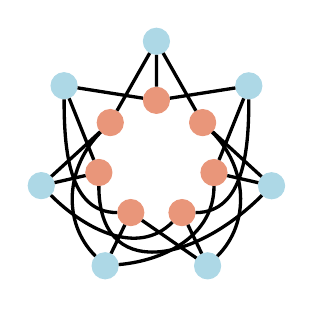
\begin{tikzpicture}[scale=0.75]

    \def\degree{51.42}
    \foreach \y/\colour in {1/lightred,2/lightblue}
    {
        \foreach \x in {0,...,6}
        {
            \node[vertex,\colour,fill=\colour] (p\y\x) at (\x*\degree+90:\y) {};
        }
    }\draw[edge] (p10) -- (p20) -- (p11) -- (p22) -- (p12) -- (p21) -- (p10) -- (p26) -- (p15) -- (p25) -- (p16) -- (p20);
    \path[edge] (p21) to[out=-90,in=180] (p13);
    \path[edge] (p13) -- (p24);
    \path[edge] (p24) to[out=45,in=-45] (p16);
    \draw[edge] (p26) to[out=-90,in=0] (p14);
    \draw[edge] (p14) to[out=-135,in=-45] (p22);
    \draw[edge] (p15) to[out=-90,in=5] (p23);
    \draw[edge] (p23) to[out=135,in=-135] (p11);
    \draw[edge] (p12) to[out=-90,in=-135,looseness=1.5] (p25);
    \draw[edge] (p13) -- (p23);
    \draw[edge] (p14) -- (p24);
\end{tikzpicture}
         \end{center}
        \subcaption{$\leviFano$.}
        \label{small-cc:leviFano/fig}
    \end{subfigure}
    \hfil
    \begin{subfigure}[]{.24\textwidth}
        \begin{center}
            

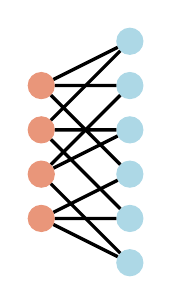
\begin{tikzpicture}[scale=0.75]

    \foreach \x in {0,...,3}
    {
        \node[vertex,lightred,fill=lightred] (r\x) at (0,3*\x/4) {};
    }
    \foreach \x in {0,...,5}
    {
        \node[vertex,lightblue,fill=lightblue] (b\x) at (1.5,3*\x/4-0.75) {};
    }
    \draw[edge] (r0) -- (b0) -- (r1) -- (b3) -- (r2) -- (b5) -- (r3) -- (b2) -- (r0);
    \draw[edge] (r0) -- (b1) -- (r2);
    \draw[edge] (r1) -- (b4) -- (r3);

\end{tikzpicture}
         \end{center}
        \subcaption{$\interspaceFourSix$.}
        \label{small-cc:graph-between-4cc-6cc/fig}
    \end{subfigure}
    \caption{Special graphs.}
    \label{small-cc:special-interspaces/fig}
\end{figure}

The incidence graph (or Levi graph) of the Fano plane~$\leviFano$ is a bipartite graph on two parts~$R$ and~$B$ each of size~$7$.
The set of arcs~$\arcs(\leviFano)$ is, up to isomorphism, determined by following property:
for each~$X \in \{R,B\}$ and~$v,v'\in X$ there is exactly one~$w \in (R \cup B) \setminus X$ for which~$vw,v'w \in \arcs(\leviFano)$.
The graph~$\leviFano$ is shown in Figure~\ref{small-cc:special-interspaces/fig}(\subref{small-cc:leviFano/fig}).
The graph~$\interspaceFourSix$ is the graph obtained form~$K_4$ by subdividing every edge.
It is a bipartite graph with vertex set~$R \disjointUnion B$ where~$\abs{R} = 4$ and~$\abs{B} = 6$.
For every~$\{r,r'\} \subsetneq R$ there is exactly one~$b \in B$ such that~$rb,r'b \in \arcs(\interspaceFourSix)$.
Figure~\ref{small-cc:special-interspaces/fig}(\subref{small-cc:graph-between-4cc-6cc/fig}) depicts~$\interspaceFourSix$.

 

\section{Critical Configurations}
\label{critical-graph/sec}

\begin{definition}
\label{def:critical-graph}
    We call a coherent configuration~$\coherentConfig$ \emph{critical} if~$\wldim{\coherentConfig}\geq 2$ and  there is no set of fibers~$\mathcal{R} \subsetneq \fibers{\coherentConfig}$ such that~$\wldim{\coherentConfig - \bigcup_{R \in \mathcal{R}} R} = \wldim{\coherentConfig}$.
\end{definition}


\begin{lemma}
\label{crictial:quotientGraph-connected/lem} \label{critical:disjoint-union/lem}
    Let~$\coherentConfig$ be a coherent configuration.
    If~$\coherentConfig$ is critical, then~$\quotientGraph{\coherentConfig}$ is connected.
\end{lemma}
\begin{proof}[Proof sketch]
    Since~$\wldim{\coherentConfig}= \max \{\wldim{\coherentConfig}[C]\mid  \text{$C$ a connected component of~$\quotientGraph{\coherentConfig}$}\}$, $\quotientGraph{\coherentConfig}$ must consist of exactly one connected component.
\end{proof}


\begin{lemma}
\label{critical:star/lem}
    Let~$\coherentConfig$ be a coherent configuration.
    If~$\coherentConfig$ is critical, then there are no distinct fibers~$R,B \in \fibers{\coherentConfig}$ with~$\minimalDegree{B}{R}=1$, that is, fibers with~$\disjointCliques{\abs{R}}{1,\frac{\abs{B}}{\abs{R}}} \in \interspace{R}{B}$.
\end{lemma}
\begin{proof}[Proof sketch]
    We argue that~$\wldim{\coherentConfig-R} \geq \wldim{\coherentConfig}$.
    Recall that we can interpret coherent configuration as complete colored graphs.
    Suppose that~$\coherentConfig' \simeq_k \coherentConfig$.
    We can assume that the two configurations are defined on the same vertex set and their vertex colorings agree.
    Then~$\coherentConfig'[\vertices(\coherentConfig)-B] \simeq_k  \coherentConfig[\vertices(\coherentConfig)-B]$.

    It suffices now to observe that an isomorphism~$\varphi$ from~$\coherentConfig'[\vertices(\coherentConfig)-B]$ to~$\coherentConfig[\vertices(\coherentConfig)-B]$ extends to an isomorphism~$\widehat{\varphi}$ from~$\coherentConfig'$ to~$\coherentConfig$. The extension is defined as follows.
    Let~$U$ be a basis relation in~$\interspace{R}{B}$ such that~$(R \cup B, U)$ is isomorphic to~$\disjointCliques{\abs{R}}{1,\nicefrac{|B|}{|R|}}$.
    For vertex~$r\in R$ choose a neighbor~$b$ in~$B$ with respect to~$U$.
    Set~$\widehat{\varphi}(r)$ to be the unique neighbor with respect to~$U$ of~$\varphi(b)$. Since criticality requires~$\wldim{\coherentConfig}\geq 2$, it follows from coherence that~$\widehat{\varphi}(r)$ is an isomorphism.
\end{proof}


\begin{lemma}
\label{critical:cycle/lem}
    Let~$\coherentConfig$ be a coherent configuration.
    If~$\coherentConfig$ is critical, then there are no fibers~$R,B\in \fibers{\coherentConfig}$ with~$|R|=|B|$ odd such that~$\minimalDegree{R}{B}=2$.
    In particular, if~$\coherentConfig$ is critical, then there is no interspace~$\disjointCycles{t}{2x} \in \interspace{R}{B}$ for positive integers~$t,x$ with~$x$ odd.
\end{lemma}
\begin{proof}
    Recall that~$\wltwo$ is able to measure lengths of paths of particular colors between two vertices, and in particular, color-alternating paths between two vertices. Under the assumptions, for all~$r \in R$ there is a unique~$b \in B$ such that there are two color-alternating paths between~$R$ and~$B$ of equal length.
    By Property~\ref{coherent-config:wl2}, the arcs~$rb$ form a basis relation of~$\coherentConfig$, and thus~$\disjointCliques{\abs{R}}{1,1} \in \interspace{R}{B}$.
    This contradicts Lemma~\ref{critical:star/lem}.
\end{proof}


A fiber~$R$ of a coherent configuration is called~\emph{large} if~$8 \leq \abs{R}$, \emph{small} if~$4 \leq \abs{R} \leq 7$, and~\emph{tiny} if~$\abs{R} \leq 3$.
Thinking of red, blue and yellow, we will typically use the letters~$R$,~$B$ and~$Y$ for fibers in general. We will use~$L$ or~$S$ to indicate that the fiber in question is large or small, respectively.


\begin{lemma}
\label{critical:tiny-CC/lem}
    Let~$\coherentConfig$ be a coherent configuration.
    If~$\coherentConfig$ is critical, then there is no tiny fiber in~$\fibers{\coherentConfig}$.
\end{lemma}
\begin{proof}
    Let~$R \in \fibers{\coherentConfig}$ be a tiny fiber. It cannot be that $R$ is the only fiber of~$\coherentConfig$ since otherwise we would have~$ \wldim{\coherentConfig}=1$.
    If~$\abs{\interspace{R}{B}} > 1$, then~$\disjointCliques{\abs{R}}{1,\nicefrac{\abs{B}}{\abs{R}}} \in \interspace{R}{B}$ contradicting Lemma~\ref{critical:star/lem}.
    So all interspaces incident to~$R$ in~$\quotientGraph{\coherentConfig}$ are homogeneous which contradicts that the quotient graph is connected (Lemma~\ref{crictial:quotientGraph-connected/lem}).
\end{proof}


Let~$\mathcal{R}$ be a union of fibers of~$\coherentConfig$, and let~$\mathcal{B}$ be the union of fibers that are not in~$\mathcal{R}$ but adjacent (in~$\quotientGraph{\coherentConfig}$) to some fiber in~$\mathcal{R}$.
We call~$\mathcal{R}$ \emph{restorable} if every automorphism of~$\coherentConfig[\mathcal{B}]$ that extends to an automorphism of
$\coherentConfig-\mathcal{R}$ also extends to an automorphism of~$\coherentConfig[\mathcal{R} \cup \mathcal{B}]$.


\begin{lemma}
\label{critical:restorable/lem}
    Let~$\coherentConfig$ be a coherent configuration.
    If~$\coherentConfig$ is critical, then there is no restorable union of fibers that is non-dominating.
\end{lemma}
\begin{proof}
    Let~$\mathcal{R}$ be a non-dominating restorable union of fibers in a
    critical coherent configuration~$\coherentConfig$. Let~$\mathcal{B}$ be the union of fibers that are not in~$\mathcal{R}$ but adjacent (in~$\quotientGraph{\coherentConfig}$) to some fiber in~$\mathcal{R}$. Define~$k\coloneqq\max \{ \wldim{\coherentConfig[\mathcal{R}\cup \mathcal{B}]},\wldim{\coherentConfig-\mathcal{R}} \}$. We argue that~$k= \wldim{\coherentConfig}$, which proves the statement.
    Recall that we can interpret coherent configuration as complete colored graphs.
    So let~$\coherentConfig'$ be a second coherent configuration for which~$(\coherentConfig,\chi)\simeq_k (\coherentConfig',\chi')$ with suitable colorings~$\chi$ and~$\chi'$. Set~$\mathcal{R}'\coloneqq\coloring'^{-1}{\coloring(\mathcal{R})}$
    and~$\mathcal{B}'\coloneqq\coloring'^{-1}{\coloring(\mathcal{B})}$ to be the vertices in~$\coherentConfig'$ in classes corresponding to~$\mathcal{R}$ and~$\mathcal{B}$, respectively.
    By the choice of~$k$ there is an isomorphism~$\varphi$ from~$\coherentConfig-\mathcal{R}$ to~$\coherentConfig'-\mathcal{R}'$ and an isomorphism~$\psi$ from~$\coherentConfig[\mathcal{R}\cup \mathcal{B}]$ to~$\coherentConfig'[\mathcal{R}'\cup \mathcal{B}']$.
    The restriction~$\psi^{-1}(\varphi|_{\mathcal{B}})$ is an automorphism of~$\coherentConfig[\mathcal{B}]$. Since~$\mathcal{R}$ is restorable, this restriction extends to an automorphism~$\mu$ of~$ \coherentConfig[\mathcal{R}\cup \mathcal{B}]$.
    Now consider the following map~$\nu\colon \vertices(\coherentConfig)\rightarrow \vertices(\coherentConfig')$ defined by
    \[
        \nu (v) =
        \begin{cases}
                \varphi(v),   & \text{for~$v\notin \mathcal{R}\cup \mathcal{B}$}\\
                \psi(\mu(v)), & \text{otherwise.}
        \end{cases}
    \]
    To see that this map is an isomorphism from~$\coherentConfig$ to~$\coherentConfig'$, it suffices to observe that for~$b\in \mathcal{B}$ we have~$\psi(\mu(b))= \varphi(v)$, so~$\nu$ combines two isomorphism that agree on~$\mathcal{B}$. We conclude that~$\coherentConfig\cong \coherentConfig'$.
\end{proof}



Let~$R$ be a fiber of a coherent configuration. We say that a fiber~$Y$ distinct from~$R$ is \emph{taken care of (regarding restorability of~$R$)} if for every~$y\in Y$ and~$U\in \interspace{Y}{R}$ there is a fiber~$B$  different from~$R$ and~$Y$, a point~$b\in B$, and an interspace~$U_B\in \interspace{B}{R}$  such that~$bU_B\subseteq yU$.


\begin{lemma}
    \label{critical:restorable:take-care/lem}
    Let~$\coherentConfig$ be a coherent configuration with distinct fibers~$R$ and~$Y$.
    If~$Y$ is taken care of (regarding restorability of~$R$) and~$R$ is restorable in~$\coherentConfig-Y$, then~$R$ is restorable in~$\coherentConfig$.
\end{lemma}
\begin{proof}
    Let~$\mathcal{B}$ be the union of fibers that are neighbors of~$R$ in $\quotientGraph{\coherentConfig}$.
    Suppose~$\varphi$ is an automorphism of~$\coherentConfig[\mathcal{B}]$. Consider the restriction~$\varphi'\coloneqq \restr{\varphi}{\mathcal{B}\setminus{Y}}$. Since~$R$ is restorable in~$\coherentConfig-Y$ there is automorphism~$\widehat{\varphi}$ that is an extension of~$\varphi'$ to~$\coherentConfig[(\mathcal{B} \setminus Y)\cup R]$. Let~$\overline{\varphi}$ be the common extension of~$\widehat{\varphi}$ and~$\varphi'$.

    It suffices now to argue that~$\overline{\varphi}$ is an automorphism of~$\coherentConfig[\mathcal{B}\cup R]$. For this it suffices to consider non-trivial basis relations~$U\in \interspace{Y}{R}$.
    So assume~$yr \in U$.
    Since~$Y$ is taken care of, there is a fiber~$B\subseteq \mathcal{B}$ other than~$Y$, a vertex~$b\in B$, and~$U_B\in \interspace{B}{R}$ with~$bU_B\subseteq yU$. Due to coherence,~$b$ can be chosen so that~$r\in bU_B$.
    Since~$\widehat{\varphi}$ is an automorphism, we
    have that~$\widehat{\varphi}(r)\in \widehat{\varphi}(b) U_B$.

    Due to coherence we have also have
    that~$\varphi(b)U_B\subseteq \varphi(y)U$ because the color of an arc~$y'b'$ ``knows'' whether~$b'U_B\subseteq y'U$.
    We conclude that~$(\overline{\varphi}(y),\overline{\varphi}(r))\in U$.
\end{proof}


We call a vertex set~$R \subseteq \vertices(\coherentConfig)$ a~\emph{module} if for all~$b \in \vertices(\coherentConfig) \setminus R$ and all~$\arcs \in \relations(\coherentConfig)$ we have~$b\arcs \cap R \in \{\emptyset, R\}$.


\begin{lemma}
\label{critical:small-cc:module/lem}
    Let~$\coherentConfig$ be a coherent configuration that is not homogeneous.
    If~$\coherentConfig$ is critical, then there is no small fiber that can be properly partitioned into at most 3 modules.
\end{lemma}
\begin{proof}
    Let~$i \in \{2,3\}$.
    Towards a contradiction, assume that there is a small fiber~$S \in \fibers{\coherentConfig}$ which partitions into $i$~modules~$M_1,\dots,M_i$.
    By Property~\ref{coherent-config:wl2}, all these modules are of equal size~$\frac{\abs{S}}{i} \in \{2,3\}$.
    Furthermore, due to their small size, we have~$K_i \in \coherentConfig[M_j]$ for all~$j \in \{1,\dots,i\}$.
    Let~$\coherentConfig'$ be a copy of~$\coherentConfig$ in which we replace~$S$ by~$S' \coloneqq \{m_1,\dots,m_i\}$ where for all~$j \in \{1,\dots,i\}$ the vertex~$m_j$ is an arbitrary representative of~$M_j$. (So we contract the modules.)
    Since~$\wltwo$ identifies cliques and~$\interspace{M_j}{M_{j'}}$ is homogeneous for all distinct~$j,j' \in \{1,\dots,i\}$, $\wldim{\coherentConfig} = \wldim{\coherentConfig'}$.
    Combining Property~\ref{coherent-config:wl2} with the fact that~$M_j$ is a module for all~$j \in \{1,\dots,i\}$, we conclude for all~$R \in \fibers{\coherentConfig} \setminus \{S\}$ that either~$\coherentConfig'[R,S']$ is homogeneous or~$\disjointCliques{i}{\frac{\abs{R}}{i},1} \in \coherentConfig'[R,S']$.
    This contradicts the arguments used in the proof of Lemma~\ref{critical:tiny-CC/lem} which show that~$S'$ can be removed without decreasing the WL-dimension.
\end{proof}


\begin{theorem}
\label{interspace-divisor/thm}
    Let~$\coherentConfig$ be a coherent configuration.
    Suppose~$(R,B,Y)$ is an induced path in~$\quotientGraph{\coherentConfig}$, $r \in R$, $y \in Y$, $U \in \interspace{R}{B}$, and~$U' \in \interspace{Y}{B}$.
    Then~$\intDegree{U} \cdot \intDegree{U'} = \abs{B} \cdot \abs{rU \cap yU'}$.

    In particular~$\lcm\{\abs{B}, \intDegree{U}\}>1$ and~$\lcm\{\abs{B}, \intDegree{U'}\}>1$. In particular~$\abs{B}$ is not prime.
\end{theorem}
\begin{proof}
    Choose~$y \in Y$ and consider~$yU'$.
    Since~$\interspace{R}{Y}$ is homogeneous, the number~$\abs{rU \cap yU'}$ is independent of the choice of~$r \in R$ or~$y \in Y$.
    The probability that for~$r \in R$ and~$b \in B$ chosen independently uniformly at random we have~$rb \in U$ is the same as the probability that for~$r \in R$ and~$b \in yU'$ chosen independently uniformly at random we have~$rb \in U$ (because all vertices in~$B$ have the same degree with respect to~$U^\star$).
    On top of that, both probabilities are the same if we first fix an arbitrary~$r$ and then choose~$b$ only  from~$B$ or~$yU'$, respectively.
    Thus~$\frac{\intDegree{U}}{\abs{B}} = \frac{\abs{vU \cap yU'}}{\intDegree{U'}}$.

    Observe that~$\intDegree{U'} > \abs{rU \cap yU'} \geq 1$ and that~$\intDegree{U} > \abs{rU \cap y U'} \geq 1$. This the implies the second part of the theorem.
\end{proof}
     

\section{Small fibers and their interspaces}
\label{small-cc/sec}


Given an interspace~$\interspace{R}{B}$ between the fibers~$R$ and~$B$, define~$\type{\interspace{R}{B}}$ to be the collection of basis relations~$\arcs$ in a~$\interspace{R}{B}$ up to isomorphism while omitting transpose basis relation~$\arcs^\star$,~$1_R$, and~$1_B$.




\begin{table}
    \centering\def\arraystretch{1.5}\begin{tabular}{|c|l|}
        \hline
        $\abs{R}$ & $\type{\inducedCC{R}}$ \\ \hline
        1 & $(K_1)$\\ \hline
        2 & $(K_2)$\\ \hline
        3 & $(K_3)$\\ \hline
        4 & $(K_4)$,~$(C_4,2K_2)$,~$(2K_2,2K_2,2K_2)$,~$(\overrightarrow{C_4},2K_2)$\\ \hline
        5 & $(K_5)$,~$(C_5,C_5)$,~$(\overrightarrow{C_5},\overrightarrow{C_5})$, \\ \hline
        6 & $(K_6)$,~$(2 K_3,K_{3,3})$,~$(2\overrightarrow{C_3},K_{3,3})$,~$(3 K_2,K_{2,2,2})$,~$(3K_2,\overrightarrow{C_3}[K_2])$,\\
            & $(C_6,3K_2,2K_3)$,~$(\overrightarrow{C_6},2\overrightarrow{C_3},3K_2)$,~$(3K_2,3K_2,\overrightarrow{2C_3},3K_2)$\\ \hline
        7 & $(K_7)$,~$(C_7,C_7,C_7)$,~$(PTr(7))$,~$(\overrightarrow{C_7},\overrightarrow{C_7},\overrightarrow{C_7})$ \\ \hline
    \end{tabular}
    \caption{Classification of all homogeneous coherent configuration of order~$n \leq 7$.}
    \label{small-cc:classificaiton-small-cc/tab}
\end{table}
 

\begin{lemma}
\label{small-cc:induced-cc/lem} \label{small-cc:implied-cc/lem}
    Every small fiber~$R$ in a coherent configuration induces, up to isomorphism, one of 22 coherent configurations. These 22 options are given in Table~\ref{small-cc:classificaiton-small-cc/tab}.
\end{lemma}
\begin{proof}
    Observe that~$(R,\inducedCC{R})$ is a homogeneous coherent configuration.
    Small homogeneous coherent configuration have been classified, see for example~\cite{MiyamotoHanaki2000,DBLP:journals/dm/HanakiM03}.
\end{proof}


Note that for small fibers, the constituents of the induced homogeneous coherent configuration contained within a fiber determine the isomorphism type of said homogeneous coherent configuration.
(This is not necessarily the case for larger fibers.)


\begin{figure}[tbp]
    \centering
    \begin{subfigure}[]{.23\textwidth}
        \begin{center}
            

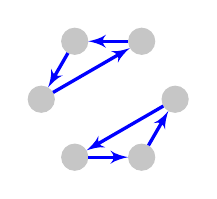
\begin{tikzpicture}[scale=0.85]

    \def\degree{60}

    \foreach \x in {0,...,5}
    {
        \node[vertex,lightgray,fill=lightgray] (p\x) at (\x*\degree+60:1) {};
    }
    \draw[arrow,blue]
        (p0) edge (p1)
        (p1) edge (p2)
        (p2) edge (p0);
    \draw[arrow,blue]
        (p3) edge (p4)
        (p4) edge (p5)
        (p5) edge (p3);
\end{tikzpicture}
         \end{center}
        \subcaption{$(2\overrightarrow{C_3},K_{3,3})$.}
        \label{small-cc:6cc:directed-2K3/fig}
    \end{subfigure}
    \hfil
    \begin{subfigure}[]{.23\textwidth}
        \begin{center}
            

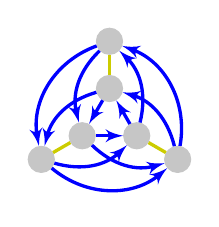
\begin{tikzpicture}[scale=0.4]
    \node[vertex,lightgray,fill=lightgray] (p0) at (90:1) {};
    \node[vertex,lightgray,fill=lightgray] (p1) at (90:2.5) {};
    \node[vertex,lightgray,fill=lightgray] (p2) at (210:1) {};
    \node[vertex,lightgray,fill=lightgray] (p3) at (210:2.5) {};
    \node[vertex,lightgray,fill=lightgray] (p4) at (330:1) {};
    \node[vertex,lightgray,fill=lightgray] (p5) at (330:2.5) {};
    \draw[arrow,blue]
        (p0) edge (p2)
        (p2) edge (p4)
        (p4) edge (p0);
    \draw[arrow,blue, bend right=40]
        (p1) edge (p3)
        (p3) edge (p5)
        (p5) edge (p1);
    \draw[arrow,blue, bend right]
        (p0) edge (p3)
        (p3) edge (p4)
        (p4) edge (p1)
        (p1) edge (p2)
        (p2) edge (p5)
        (p5) edge (p0);

    \draw[edge,darkyellow] (p0) -- (p1);
    \draw[edge,darkyellow] (p2) -- (p3);
    \draw[edge,darkyellow] (p4) -- (p5);

\end{tikzpicture}
         \end{center}
        \subcaption{$(\overrightarrow{C_3}[K_2],3K_2)$.}
        \label{small-cc:6cc:wreath/fig}
    \end{subfigure}
    \hfil
    \begin{subfigure}[]{.27\textwidth}
        \begin{center}
            

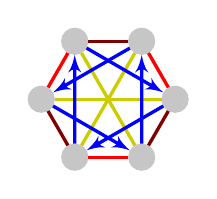
\begin{tikzpicture}[scale=0.85]

    \def\degree{60}

    \foreach \x in {0,...,5}
    {
        \node[vertex,lightgray,fill=lightgray] (p\x) at (\x*\degree+60:1) {};
    }
    \draw[edge,darkred] (p0) -- (p1);
    \draw[edge,darkred] (p2) -- (p3);
    \draw[edge,darkred] (p4) -- (p5);

    \draw[edge,red] (p1) -- (p2);
    \draw[edge,red] (p3) -- (p4);
    \draw[edge,red] (p5) -- (p0);

    \draw[edge,darkyellow]
        (p0) edge (p3)
        (p1) edge (p4)
        (p5) edge (p2);

    \draw[arrow,blue]
        (p0) edge (p2)
        (p2) edge (p4)
        (p4) edge (p0);
    \draw[arrow,blue]
        (p1) edge (p5)
        (p5) edge (p3)
        (p3) edge (p1);
\end{tikzpicture}
         \end{center}
        \subcaption{$(3K_2,3K_2,2\overrightarrow{C_3},3K_2)$.}
        \label{small-cc:6cc:alternating-C6/fig}
    \end{subfigure}
    \hfil
    \begin{subfigure}[]{.23\textwidth}
        \begin{center}
            

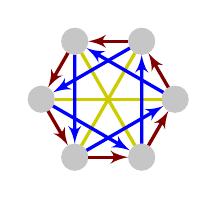
\begin{tikzpicture}[scale=0.85]

    \def\degree{60}

    \foreach \x in {0,...,5}
    {
        \node[vertex,lightgray,fill=lightgray] (p\x) at (\x*\degree+60:1) {};
    }
    \draw[arrow,darkred]
        (p0) edge (p1)
        (p1) edge (p2)
        (p2) edge (p3)
        (p3) edge (p4)
        (p4) edge (p5)
        (p5) edge (p0);

    \draw[edge,darkyellow] (p0) -- (p3);
    \draw[edge,darkyellow] (p1) -- (p4);
    \draw[edge,darkyellow] (p5) -- (p2);

    \draw[arrow,blue]
        (p0) edge (p2)
        (p2) edge (p4)
        (p4) edge (p0);
    \draw[arrow,blue]
        (p1) edge (p3)
        (p3) edge (p5)
        (p5) edge (p1);
\end{tikzpicture}
         \end{center}
        \subcaption{$(\overrightarrow{C_6},2\overrightarrow{C_3},3K_2)$.}
        \label{small-cc:6cc:directed-C6/fig}
    \end{subfigure}
    \caption{Coherent configurations of order~$6$ with directed edges.}
    \label{small-cc:6cc:coherent-config/fig}
\end{figure}


\begin{lemma}
    \label{small-cc:interspace/lem}
    Let~$\coherentConfig$ be a coherent configuration, and let~$(R,B)$ be an edge in~$\quotientGraph{\coherentConfig}$ such that~$2 \leq \abs{R} \leq \abs{B} \leq 7$.
    \begin{enumerate}[label=(\arabic*)]
        \item If~$\abs{R} = 2$,
        then~$\abs{B} \in \{2,4,6\}$ and~$\disjointCliques{2}{1,\frac{\abs{B}}{2}} \in \interspace{R}{B}$.
        \item If~$\abs{R} = 3$,
        then~$\abs{B} \in \{3,6\}$ and~$\disjointCliques{3}{1,\frac{\abs{B}}{2}} \in \interspace{R}{B}$.
        \item If~$\abs{R} = 4$, then~$\abs{B} \in \{4,6\}$.
        Furthermore, if~$\abs{R} = 4$ and~$\abs{B} = 4$, then at least one of the constituents~$\cycle{8}$, $\matching{4}$, and~$\disjointCliques{2}{2,2}$ is contained in~$\interspace{R}{B}$, and if~$\abs{R} = 4$ and~$\abs{B} = 6$, then at least one of constituents~$\interspaceFourSix$ and~$\disjointCliques{2}{2,3}$ is contained in~$\interspace{R}{B}$.
        \item If~$\abs{R} = 5$,
        then~$\abs{B} = 5$ and~$\matching{5} \in \interspace{R}{B}$.
        \item If~$\abs{R} = 6$,
        then~$\abs{B} = 6$ and at least one of constituents~$\matching{6}$, $\cycle{12}$, $\disjointCliques{3}{2,2}$, or~$\disjointCliques{2}{3,3}$ is contained in~$\interspace{R}{B}$.
        \item If~$\abs{R} = 7$,
        then~$\abs{B} = 7$ and at least one of constituents~$\matching{7}$ and~$\leviFano$ is contained in~$\interspace{R}{B}$.
    \end{enumerate}
\end{lemma}
\begin{proof}
    The claims for~$\abs{R},\abs{B} \in \{1,\dots,4\}$ have been determined in \cite[Figures 2 and 3]{DBLP:journals/siamdm/FuhlbruckKV21}.
    Let~$U \in \interspace{R}{B}$ be such that~$\intDegree{U} = \minimalDegree{R}{B}$.
    Note that~$\intDegree{U} \in \{1,\dots,\lfloor \frac{\abs{B}}{2} \rfloor\}$.
    The constituent~$(R \disjointUnion B, U)$ satisfies~
    \begin{equation}
    \label{interspace:handshake/eq}
        \abs{R}\intDegree{U} = \abs{B} \intDegree{U^\star},
    \end{equation}
    and thus~$\intDegree{U^\star} \in \{1,\dots,\lfloor \frac{\abs{R}}{2} \rfloor\}$.
    Note~$\intDegree{U} = \intDegree{U^\star}$ if~$\abs{R} = \abs{B}$, and in  particular, the interspace~$\matching{\abs{R}} \in \interspace{R}{B}$ appears if~$\intDegree{U} = 1$.

    Now assume~$\abs{R} \leq 4 < \abs{B}$.
    If~$\abs{R} = 2$ (respectively~$\abs{R} = 3$), then by Equation~\eqref{interspace:handshake/eq} the size of~$B$ is~$6$ and~$\intDegree{U} = 3$ (respectively~$\intDegree{U} = 2$).
    Thus~$\disjointCliques{2}{1,3} \in \interspace{R}{B}$ (respectively~$\disjointCliques{3}{1,2} \in \interspace{R}{B}$).
    If~$\abs{R} = 4$, then~$\abs{B} = 6$,~$\intDegree{U} = 3$, and~$\intDegree{U^\star} = 2$.
    If there are distinct~$b,b' \in B$ such that~$bU^\star = b'U^\star$, then~$\disjointCliques{2}{2,3} \in \interspace{R}{B}$.
    Otherwise, for all distinct~$r,r' \in R$ there is a~$b$ with~$bU^\star = \{r,r'\}$.
    Hence~$\clique{4} \in \inducedCC{R}$ and~$\interspaceFourSix \in \interspace{R}{B}$.

    By Equation~\eqref{interspace:handshake/eq}, if~$\abs{R} = 5$, then~$\abs{B} = 5$ and~$\intDegree{U} = 2$.
    Due to Property~\ref{coherent-config:wl2}, we have~$\cycle{10} \in \interspace{R}{B}$ and~$\matching{5} \in \interspace{R}{B}$.

    In the upcoming cases of~$\abs{R} \in \{6,7\}$, a finer case distinction will be necessary.
    So for the rest of the proof, let~$G$ be a constituent which is contained in~$\inducedCC{R}$, and let~$r,r'\in  R$ be such that~$rr' \in \arcs(G)$.
    Further, define~$s \coloneqq \abs{rU \cap r'U}$. We will repeatedly use the following \emph{coherence criterion}:
    if~$d(G)$ is the degree of the graph underlying~$G$, then~$d(G)\cdot s$ is a multiple of~$d(U)$.

    Assume~$\abs{R} = 6$. By Equation~\eqref{interspace:handshake/eq} we know that~$\abs{B} = 6$.
    If~$\intDegree{U} = 2$, then at least one of the following constituents is contained in~$\interspace{R}{B}$:
    $\cycle{12}$, $\disjointCliques{3}{2,2}$, or~$2\cycle{6}$.
    In the last case, we also have~$\matching{6} \in \interspace{R}{B}$ due to Property~\ref{coherent-config:wl2}.
    All other possible constituents imply a violation of Property~\ref{coherent-config:wl2}.
    Assume now that~$\intDegree{U} = 3$:

    \begin{enumerate}[label=(\arabic*)]
        \item
        $G \cong \clique{6}$.
        We will double count how many arcs from~$U$ have an endpoint in~$rU$:
        recall that~$\intDegree{U} = \intDegree{U^\star} = 3$ since~$\abs{R} = \abs{B}$.
        Thus there are~$\sum_{b \in rU} 3 = 9$ such arcs.
        On the other hand, there are~$3$ such arcs which start in~$r$.
        Furthermore, each~$r' \in R\setminus\{r\}$ has exactly~$s$ common neighbors with~$r$, so~$5s$ arcs that do not start in~$r$.
        Together, we have~$3+5s \neq 9$ for all~$s \in \{0,\dots,3\}$.
        Thus we obtain a contradiction.

        \item
        $G \cong \cycle{6}$ or~$G \cong \overrightarrow{C_6}$.
        We have~$d(G)\in \{1,2\}$ and~$d(U)=3$. So~$s\notin \{1,2\}$ by the coherence criterion. If~$s=3$, then, since~$G$ is connected, all vertices of~$R$ would have the same neighbors under~$U$ in~$B$ which violates coherence. If~$s=0$, then~$U$ forms an~$\disjointCliques{2}{3,3}$ interspace.

        \item
        $G \cong \disjointCliques{2}{3}$ or~$G \cong 2\overrightarrow{\cycle{3}}$.
        Due to the coherence criterion~$s \notin \{1,2\}$.
        Also~$s=0$ is impossible since three vertices cannot have pairwise non-adjacent neighborhoods under~$U$ each covering half the vertices of~$B$.
        If~$s = 3$, then~$\disjointCliques{2}{3,3} \in \interspace{R}{B}$.

        \item
        $G \cong \matchingCC{3}$. Due to the coherence criterion~$s\notin \{1,2\}$.
        A contradiction of Equation~\eqref{interspace:handshake/eq} is implied if~$s = 3$ because then vertices of~$B$ have an even number of incoming arcs from~$U$.
        Suppose~$s = 0$ and let~$r'',r''' \in R$ such that~$r''r''' \in \arcs(G)$.
        If~$\abs{r U \cap r''U} \in \{0,3\}$, then~$\disjointCliques{2}{3,3} \in \interspace{R}{B}$.
        If~$\abs{r U \cap r''U} \in \{1,2\}$, then~$\abs{r U \cap r''U} = \abs{r' U \cap r'''U}$ and implying that~$\cycle{6} \in \inducedCC{B}$.
    \end{enumerate}

    Assume~$\abs{R} = \abs{B} = 7$.
    If~$\intDegree{U} = 2$, then~$\cycle{14} \in \interspace{R}{B}$ and~$\matching{7} \in \interspace{R}{B}$.
    So assume~$\intDegree{U} = 3$.

    \begin{enumerate}[label=(\arabic*)]
        \item
        $G \cong \clique{7}$.
        We will double count how many arcs from~$U$ have an endpoint in~$rU$:
        recall that~$\intDegree{U} = \intDegree{U^\star} = 3$ since~$\abs{R} = \abs{B}$.
        Thus we have~$\sum_{b \in rU} 3 = 9$.
        On the other hand, there are~$3$ ingoing arcs which start in~$r$.
        Furthermore, each~$r' \in R\setminus\{r\}$ has exactly~$s$ common neighbors with~$r$ so~$6s$ arcs that do not start in~$r$.
        Together, we have~$3+6s \neq 9$ for all~$s \in \{0,2,3\}$.
        If~$s = 1$, then~$\leviFano \in \interspace{R}{B}$ since the interspace satisfies the combinatorial properties of a projective plane.

        \item
        $G \cong \cycle{7}$ or~$G \cong \overrightarrow{\cycle{7}}$.
        As before, since~$G$ is connected, $s = 3$ is impossible.
        By the coherence criterion~$s\notin \{1,2\}$.
        In fact, this means that $\abs{\overline{r}U \cap \overline{r'}U} = 0$ for all~$\overline{r},\overline{r'}\in R$ since each such pair forms an arc in some constituent of~$R$ isomorphic to~$\cycle{7}$ or~$\overrightarrow{\cycle{7}}$ (See Table~\ref{small-cc:classificaiton-small-cc/tab}). This is however a contradiction since~$7$ is not divisible by~$3$.

        \item
        $G \cong PTr(7)$. Recall that~$G$ is a complete oriented graph.
        If~$s = 3$, all vertices of~$R$ have the same neighbors under~$U$ since~$G$ is connected, so the interspace is trivial.
        If~$s = 1$, then~$\leviFano \in \interspace{R}{B}$, because the combinatorial properties of a projective plane are fulfilled. Suppose~$R = \{r_1,\dots,r_7\}$.
        If~$s = 0$, then~$r_1U \cap r_2U = \emptyset$ and~$r_1U \cap r_3U = \emptyset$.
        This implies~$r_3U \cap r_2U \neq \emptyset$, a contradiction.
        Finally if~$s=2$ then at least~$2\cdot 7=14$ of the arcs from~$U$ end in~$r_1U$.
        But only~$|r_1U|\cdot d(U^\star)= 3\cdot 3=9$ of the arcs from~$U$ can end in~$r_1U$.\qedhere
    \end{enumerate}
\end{proof}




\begin{table}
    \centering\def\arraystretch{1.2}\begin{tabular}{|c|c|l|}
        \hline
        $\abs{R}$ & $\abs{B}$ & $\type{\interspace{R}{B}}$ \\ \hline
        4 & 4 & $(\cycle{8}, \cycle{8})$, $(\disjointCliques{2}{2,2}, \disjointCliques{2}{2,2})$\\ \hline
        4 & 6 & $(\interspaceFourSix, \interspaceFourSix)$, $(\disjointCliques{2}{2,3},\disjointCliques{2}{2,3})$\\ \hline
        6 & 6 & $(\cycle{12}, \cycle{12}, \disjointCliques{3}{2,2})$, $(\disjointCliques{2}{3,3},\disjointCliques{2}{3,3})$, $(\disjointCliques{3}{2,2}, \disjointCliques{3}{2,2}, \disjointCliques{3}{2,2})$, $(\disjointCliques{3}{2,2},R \times B - \disjointCliques{3}{2,2})$ \\ \hline
        7 & 7 & $(\leviFano, R \times B -\leviFano)$ \\ \hline
    \end{tabular}
    \caption{Classification of all~$\interspace{R}{B}$ with~$2 \leq \abs{R} \leq \abs{B} \leq 7$ in critical coherent configurations.}
    \label{small-cc:classificaiton-small-interspaces/tab}
\end{table}
 

To classify all possible isomorphism types of interspaces between small fibers, we can examine the coarsest coherent configurations containing one of the graphs guaranteed to exists by Lemma~\ref{small-cc:interspace/lem} as constituent. Table~\ref{small-cc:classificaiton-small-interspaces/tab} lists all isomorphism types between two small fibers in a critical coherent configuration. Note that the isomorphism type is determined by the isomorphism types of its constituents. (This is not necessarily the case for interspaces between larger fibers). For fibers of size~$4$ and~$6$ the classification can alternatively derived from the upcoming Theorem~\ref{global-argument:large-small-interspace:classification}.


\begin{lemma}
\label{small-cc:interspace-implies-cc/lem}
    Let~$\coherentConfig$ be a coherent configuration, and let~$(R,B)$ be an edge in~$\quotientGraph{\coherentConfig}$ with~$\abs{R} \leq \abs{B}$, and suppose~$x \in \{4,6\}$ and~$y \in \{2,3\}$.
    \begin{enumerate}[label = (\arabic*)]
        \item
        If~$\cycle{2x} \in \interspace{R}{B}$, then~$\cycle{x} \in \inducedCC{R}$.
        \item
        If~$y\clique{2,2} \in \interspace{R}{B}$, then~$\disjointCliques{y}{2} \in \inducedCC{R}$.
        \item
        If~$\disjointCliques{2}{2,3} \in \interspace{R}{B}$, then~$\matchingCC{2} \in \inducedCC{R}$ and either~$\disjointCliques{2}{3} \in \inducedCC{B}$ or~$2\overrightarrow{C_3} \in \inducedCC{B}$.
        \item
        If~$\disjointCliques{2}{3,3} \in \interspace{R}{B}$, then either~$\disjointCliques{2}{3} \in \inducedCC{R}$ or~$2\overrightarrow{\cycle{3}} \in \inducedCC{B}$.
        \item
        If~$\leviFano \in \interspace{R}{B}$, then either~$\clique{7} \in \inducedCC{R}$ or~$PTr(7) \in \inducedCC{R}$.
        \item
        If~$\interspaceFourSix \in \interspace{R}{B}$, then~$\clique{4} \in \inducedCC{R}$ and either~$\matchingCC{3}, K_{2,2,2} \in \inducedCC{B}$ or~$\matchingCC{3},\overrightarrow{\cycle{3}}[\clique{2}] \in \inducedCC{B}$.
    \end{enumerate}
\end{lemma}
\begin{proof}
    The first five claims follow from Property~\ref{coherent-config:wl2} and from the proof of Lemma~\ref{small-cc:interspace/lem}.
    Consider the last claim and suppose~$U \in \interspace{R}{B}$ with~$(R \disjointUnion B, U) \cong \interspaceFourSix$.
    Then~$\clique{4} \in \inducedCC{R}$ since otherwise~$R$ violates Property~\ref{coherent-config:wl2}.
    For all~$r \in R$ the neighborhood~$rU$ induces up to isomorphism the same subgraph in~$\inducedCC{B}$.
    Thus either~$\clique{3} \in \inducedCC{rU}$ or~$\overrightarrow{\cycle{3}} \in \inducedCC{rU}$.
    In the first case~$\clique{2,2,2} \in \inducedCC{B}$, in the latter case~$\overrightarrow{\cycle{3}}[\clique{2}]$.
\end{proof}




     

\section{Interspaces between large and small fibers}
\label{interspace-large-small/sec}

To study interspaces between large and small fibers we will introduce a specialized notation that concisely captures the attachment structure that vertices in the large fiber have in the small fiber.
The challenge is to capture the entire information for all constituents simultaneously.

For a relation~$\arcs$, we define~$\ul(\arcs)$ to be~$\arcs \cup \arcs^\star$.
We extend this notation to graphs and coherent configurations to obtain their \emph{underlying undirected structure}.
For a coherent configuration~$\coherentConfig$, we set~$\ul(\coherentConfig)$ to be~$(\vertices(\coherentConfig), \{\ul(\arcs) \mid \arcs \in \relations(\coherentConfig)\})$.
Observe that~$\ul(\coherentConfig)$ is not necessarily coherent.
For a graph~$G$, we set~$\ul(G)$ to be~$(\vertices(G), \ul(\arcs(G)))$ and call it the \emph{underlying undirected graph} of~$G$.

Let~$L,S$ be distinct fibers of a coherent configuration~$\coherentConfig$.
We say the interspace~$\interspace{L}{S}$ contains the \emph{interspace pattern} $(G^1, d^1_1, d^1_2, \dots, d^1_{t_1}; \dots; G^k, d^k_1, d^k_2, \dots, d^k_{t_k})$ if~$\sum_{j = 1}^{k} t_j = \abs{\interspace{L}{S}} - 1$, there are distinct~$\arcs^1, \dots, \arcs^k \in \inducedCC{S}$ such that for each~$i \in \{1,\dots,k\}$ we have~$\ul(S,\arcs^i) \cong G^i$, and there are distinct~$U^i_1, \dots, U^i_{t_i} \in \interspace{L}{S}$ such that for all~$\ell \in L$ and~$j \in \{1, \dots, t_i\}$ the set~$\ell U^i_j$ induces a~$d^i_j$-clique in~$\ul(S,A^i)$. We should emphasize that the sum of the~$t_i$ is~$\abs{\interspace{L}{S}} - 1$ and thus we omit exactly one of the interspaces in the pattern. In fact, in general the missing interspace will not satisfy a clique condition. Also, it is a priori not clear that an interspace always has a pattern of this form we just defined.

Considering~$d^i_j = 3$, if for all~$S' \subseteq S$ that induce a~$3$-clique in~$\ul(S,A^1)$ the common neighborhood~$\bigcap_{s \in S'} s {U^i_j}^\star$ is not empty, then we mark the entry in the interspace pattern by~$^\dag$. This means there is a vertex in~$\ell\in L$ such that~$\ell U^i_j= S'$.
On the other hand, if  for all~$S' \subseteq S$ inducing a~$3$-clique in~$\ul(S,A^1)$ we have that~$S\setminus S'$ is a also~$3$-clique and exactly one of~$\bigcap_{s \in S'} s {U^i_j}^\star$ or~$\bigcap_{s \in S \setminus S'} s {U^i_j}^\star$ is not empty, then we mark the entry by~$^\ddag$.
For example, the interspace pattern~$(\clique{2,2,2},3)$ has two subpatterns, namely~\ipsixMatchingComplement\xspace and~\ipsixMatchingComplementD. In principle there could be other subcases, but it will follow from our classification that only these two subcases arise.


\begin{theorem}
\label{global-argument:large-small-interspace:classification}
    Let~$\coherentConfig$ be a critical coherent configuration and~$(L,S)$ be an edge in~$\quotientGraph{\coherentConfig}$.
    If~$\abs{S} \in \{4,6\}$, then~$\interspace{L}{S}$ contains one of the following interspace patterns:
    \begin{multicols}{4}
        \begin{enumerate}
            \item \ipfourClique
            \item \ipfourMatching
            \item \ipfourCycle
            \item \ipsixCliqueTwo
            \item \ipsixCliqueTwoTwice
            \item \ipsixMatching
            \item \ipsixMatchingTwice
            \item \ipsixMatchingAndCycle
            \item \ipsixMatchingMatching
            \item \ipsixMatchingAndComplement
            \item \ipsixTriangleComplement
            \item \ipsixTriangleComplementTwice
            \item \ipsixCliqueThree
            \item \ipsixCliqueThreeD
            \item \ipsixTriangle
            \item \ipsixMatchingComplement
            \item \ipsixMatchingComplementD.
        \end{enumerate}
    \end{multicols}
\end{theorem}
\begin{proof}
    Since~$\abs{S} \in \{4,6\}$, we have~$\minimalDegree{L}{S} \in \{2,3\}$ and~$\abs{\interspace{L}{S}} \in \{2,3\}$.

    Let us first observe that for every basis relation~$U\in \interspace{L}{S}$ with~$|\ell U|\in \{2,3\}$ and every~$\ell \in L$ the set~$lU$ forms a clique in some undirected underlying graph of a constituent of~$\inducedCC{S}$. Indeed, from coherence, it follows that every constituent of $\inducedCC{\ell U}$ is a regular graph. Thus, since~$|\ell U|\in \{2,3\}$, there is only a single constituent, which must be a~$2$-clique or a~$3$-clique. Note that the size of the clique is independent of the choice of~$\ell$ due to coherence. Also note that, again due to coherence, the constituent that contains the clique $\inducedCC{\ell U}$ must be the same for different choices of~$\ell$.

    Finally observe that, since~$\abs{S} \in \{4,6\}$, the interspace~$\interspace{L}{S}$ contains at most one basis relation~$U \in \interspace{L}{S}$ with~$\intDegree{U} >3$.
    From these observations we conclude that~$\interspace{L}{S}$ has some an interspace pattern of the form $(G^1, d^1_1, d^1_2, \dots, d^1_{t_1}; \dots; G^k, d^k_1, d^k_2, \dots, d^k_{t_k})$.

    First assume~$\abs{S} = 4$, and thus we have~$\abs{\interspace{L}{S}} = 2$.
    Then~$k = 1$, $t_1 = 1$, and~$d^1_1 = 2$.
    If there are~$\ell \in L$ and~$U \in \interspace{L}{S}$ such that~$\ell U$ induces a clique in~$\ul(G)$ where~$G$ is constituent of~$\inducedCC{S}$ isomorphic to~$\overrightarrow{C_4}$, then~$\inducedCC{\ell U}$ is not regular.
    Therefore by Lemma~\ref{small-cc:induced-cc/lem}, each constituent~$G$ of~$\inducedCC{S}$ (and thus the undirected graph~$G^1$) is isomorphic to one of the graphs
    $\clique{4}$,~$\cycle{4}$, or~$\disjointCliques{2}{2}$.
    Observe that for all distinct~$s,s' \in S$ which are adjacent in~$G$, the two vertices in~$S \setminus \{s,s'\}$ are also adjacent in~$G$.
    Thus~$\interspace{L}{S}$ has one of the interspace patterns
    $\ipfourClique$,~$\ipfourCycle$, or~$\ipfourMatching$.

    Now assume~$\abs{S} = 6$.
    Let~$\ell \in L$,~$U \in \interspace{L}{S}$, and~$G$ be constituent of~$\inducedCC{S}$ such that~$\ell U$ induces a clique in~$\ul(G)$.
    By Lemma~\ref{small-cc:induced-cc/lem} the constituent~$G$ is isomorphic to one of the graphs $K_6$,~$2 K_3$,~$2\overrightarrow{C_3}$,~$K_{3,3}$,~$3 K_2$,~$K_{2,2,2}$,~$\overrightarrow{C_3}[K_2]$,
    $C_6$, or~$\overrightarrow{C_6}$.
    We distinguish cases according to~$G$.

    \textit{(Case~$G \cong C_6$)}.
    By Lemma~\ref{small-cc:induced-cc/lem} there must exist constituents~$G', G''$ of~$\inducedCC{S}$ such that~$G' \cong 3K_2$ and~$G'' \cong 2K_3$.
    Observe~$\intDegree{U} \neq 3$ since~$\cycle{6}$ does not contain a~$3$-clique.
    Thus~$\intDegree{U} = 2$.
    Assume~$\abs{\interspace{L}{S}} = 2$ and let~$\overline{U} \in \interspace{L}{S}$ with~$\overline{U} \neq U$.
    Then exactly two vertices in~$\ell \overline{U}$ have distance~$3$ in~$G$, which contradicts coherence.
    Thus we know that~$\abs{\interspace{L}{S}} = 3$.  So let~$\{U,\overline{U},\widetilde{U}\} = \interspace{L}{S}$.
    If both~$\ell \overline{U}$ and~$\ell \widetilde{U}$ induce $2$ cliques in~$G$, then there is exactly one pair~$(\overline{s},\widetilde{s}) \in \ell \overline{U} \times \ell \widetilde{U}$ such that~$\overline{s}\widetilde{s} \in \arcs(G')$.
    Thus by coherence~$\overline{U}$ cannot be a basis relation.
    A similar argument applies if both~$\ell \overline{U}$ and~$\ell \widetilde{U}$ induce $2$ cliques in~$G''$.
    In the last possible case,~$\ell \overline{U}$ induces a~$2$-clique in~$\ul(G')$ and~$\ell \widetilde{U}$ induces a~$2$-clique in~$\ul(G)$.
    Then~$\interspace{L}{S}$ has interspace pattern~$\ipsixMatchingAndCycle$.

    \textit{(Case~$G \cong \overrightarrow{C_6}$)}.
    Once again, observe~$\intDegree{U} \neq 3$ since~$\cycle{6}$ does not contain a~$3$-clique.
    Thus~$\intDegree{U} = 2$.
    However~$\inducedCC{\ell U}$ is not regular.

    \textit{(Case~$G \cong 2 K_3$)}.
    If~$\intDegree{U} = 2$, then~$G-\ell U$ is not regular, which contradicts coherence.     Thus~$\intDegree{U} = 3$. Then~$\interspace{L}{S}$ has interspace pattern~$(2K_3,3)$.
    To be precise, the interspace~$\interspace{L}{S}$ has the interspace subpattern~$\ipsixTriangle$:
    there are exactly two distinct vertex sets~$S',S \setminus S' \subseteq S$ inducing~$3$-cliques in~$G$ and for each vertex~$s \in S$ either~$s \in S'$ or~$s \in S \setminus S'$.
    Without loss of generality assume~$\ell U  = S'$.
    Thus by Property~\ref{coherent-config:wl2} there is~$\ell' \in L$ such that~$\ell' U = S \setminus S'$.

    \textit{(Case~$G \cong 2\overrightarrow{C_3}$)}.
    This case is analogous to the previous case.

    \textit{(Case~$G \cong K_{3,3}$)}.
    Observe~$\intDegree{U} \neq 3$ since~$K_{3,3}$ does not contain a~$3$-clique.
    Thus~$\intDegree{U} = 2$.
    By Lemma~\ref{small-cc:induced-cc/lem} there is a constituent~$G'$ in~$\inducedCC{S}$ isomorphic to either~$2K_3$ or~$2\overrightarrow{C_3}$.
    If~$|\interspace{L}{S}| = 2$, then~$\interspace{L}{S}$ has interspace pattern~$\ipsixTriangleComplement$ and~$G' \cong 2K_3$.
    So assume~$|\interspace{L}{S}| = 3$.
    Let~$\{U,\overline{U},\widetilde{U}\} = \interspace{L}{S}$.
    If~$\ell \overline{U}$ induces a~$2$-clique in~$\ul(G')$, then~$G' - \ell \overline{U}$ is not regular, which contradicts coherence.
    If~$\ell \overline{U}$ induces a~$2$-clique in~$\ul(G)$, then~$\ell \widetilde{U}$ induces a~$2$-clique in~$\ul(G)$ as well.
    Hence, the interspace~$\interspace{L}{S}$ has interspace pattern~$\ipsixTriangleComplementTwice$.

    \textit{(Case~$G \cong 3 K_2$)}.
    So~$\intDegree{U} = 2$.
    If~$|\interspace{L}{S}| = 2$, then~$\interspace{L}{S}$ has interspace pattern~$\ipsixMatching$.
    Assume~$|\interspace{L}{S}| = 3$, and let~$\{U,\overline{U},\widetilde{U}\} = \interspace{L}{S}$.
    If~$\ell \overline{U}$ induces a~$2$-clique in~$\ul(G)$, then~$\ell \widetilde{U}$ induces a~$2$-clique in~$\ul(G)$ as well.
    Hence~$\interspace{L}{S}$ has interspace pattern~$\ipsixMatchingTwice$.

    Let~$G'$ be another constituent of~$\inducedCC{S}$ such that~$\ell \overline{U}$ and~$\ell \widetilde{U}$ induce a~$2$-clique in~$\ul(G')$.
    Since we have already covered the previous cases, we can assume~$G'$ is not isomorphic to~$2K_3$, $2\overrightarrow{C_3}$, $C_6$, or~$\overrightarrow{C_6}$.
    If~$G' \cong \overrightarrow{C_3}[K_2]$, then~$\coherentConfig[\ell \overline{U}]$ is not regular.
    If~$G' \cong K_{2,2,2}$, then~$\interspace{L}{S}$ has interspace pattern~$\ipsixMatchingAndComplement$.

    Finally, let $G', G''$ be two other constituent of~$\inducedCC{S}$ such that~$\ell \overline{U}$ (respectively~$\ell \widetilde{U}$) induces a~$2$-clique in~$\ul(G')$ (respectively~$\ul(G'')$).
    Since we have already covered the previous cases, we can assume~$G'$ is not isomorphic to~$2K_3$, $2\overrightarrow{C_3}$, $C_6$, or~$\overrightarrow{C_6}$.
    If~$G'$ and~$G''$ are both isomorphic to~$3K_2$, then~$\interspace{L}{S}$ has interspace pattern~$\ipsixMatchingMatching$.

    \textit{(Case~$G \cong K_{2,2,2}$)}.
    By Lemma~\ref{small-cc:induced-cc/lem} there is one other constituent~$G'$ in~$\inducedCC{S}$ isomorphic to~$3K_2$.

    Assume~$|\interspace{L}{S}| = 2$ and~$\intDegree{U} = 2$.
    Let~$\overline{U} \in \interspace{L}{S}$ with~$\overline{U} \neq U$.
    Hence there are exactly two vertices~$s,s' \in \ell \overline{U}$ such that~$ss' \in \arcs(G)$.
    By coherence~$\overline{U}$ cannot be a basis relations of~$\interspace{L}{S}$.

    Assume~$|\interspace{L}{S}| = 3$ and let~$\{U,\overline{U},\widetilde{U}\} = \interspace{L}{S}$.
    Suppose both~$\ell \overline{U}$ and~$\ell \widetilde{U}$ induce a~$2$-clique in~$\ul(G)$.
    Then there is exactly one pair~$(\overline{s},\widetilde{s}) \in \ell \overline{U} \times \ell \widetilde{U}$ such that~$\overline{s}\widetilde{s} \in \arcs(G)$.
    By coherence~$\overline{U}$ cannot be a basis relation.
    The cases where~$\ell \overline{U}$ or~$\ell \widetilde{U}$ induce a~$2$-clique in~$\ul(G')$ are covered by the previous case.

    Finally assume~$|\interspace{L}{S}| = 2$ and~$\intDegree{U} = 3$.
    If for all induced $3$-cliques~$S'$ in~$G$ there is an~$\ell \in L$ with~$\ell U = S'$, then~$\interspace{L}{S}$ has the interspace subpattern~$\ipsixMatchingComplement$.
    Suppose that there is an induced $3$-clique~$S'$ in~$G$ such that for all~$\ell' \in L$ we have~$\ell' U \neq S'$ and~$\ell' U \neq S\setminus S'$.
    Let~$s \in S' \cap \ell U$,~$s' \in \ell U \cap (S \setminus S')$, and~$s'' \in S' \cap (S \setminus \ell U)$.
    Then~$s$ and~$s'$ have a different number of common neighbors in~$L$ under~$U$ than~$s$ and~$s''$.
    By coherence~$G$ is not a constituent of~$\inducedCC{S}$.
    If for all induced $3$-cliques~$S'$ in~$G$ there is an~$\ell \in L$ with either~$\ell U = S$ or~$\ell U = S \setminus S'$, then~$\interspace{L}{S}$ has the interspace subpattern~$\ipsixMatchingComplementD$.

    \textit{(Case~$G \cong \overrightarrow{C_3}[K_2]$)}.
    This case works similar to the previous case.

    \textit{(Case~$G \cong K_6$)}.
    If~$|\interspace{L}{S}| = 2$ and~$\intDegree{U} = 2$, then~$\interspace{L}{S}$ has interspace pattern~$\ipsixCliqueTwo$.
    If~$|\interspace{L}{S}| = 3$, then~$\interspace{L}{S}$ has interspace pattern~$\ipsixCliqueTwoTwice$.
    Finally assume~$|\interspace{L}{S}| = 2$ and~$\intDegree{U} = 3$.
    If for all induced $3$-cliques~$S'$ in~$G$ there is an~$\ell \in L$ with~$\ell U = S'$, then~$\interspace{L}{S}$ has the interspace subpattern~$\ipsixCliqueThree$.
    Suppose that there is an induced $3$-clique~$S'$ in~$G$ such that for all~$\ell' \in L$ we have~$\ell' U \neq S'$ and~$\ell' U \neq S\setminus S'$.
    Let~$s \in S' \cap \ell U$,~$s' \in \ell U \cap (S \setminus S')$, and~$s'' \in S' \cap (S \setminus \ell U)$.
    Then~$s$ and~$s'$ have a different number of common neighbors in~$L$ under~$U$ than~$s$ and~$s''$.
    Hence~$G$ is not a constituent of~$\inducedCC{S}$.
    If for all induced $3$-cliques~$S'$ in~$G$ there is an~$\ell \in L$ with either~$\ell U = S$ or~$\ell U = S \setminus S'$, then~$\interspace{L}{S}$ has the interspace subpattern~$\ipsixCliqueThreeD$.
\end{proof}


We can observe that the interspace patterns in the theorem are mutually exclusive, and we conclude the following.


\begin{corollary}
\label{large-small-interspace:classification:uniqueness/cor}
    Let~$\coherentConfig$ be a critical coherent configuration, and let~$(L,S)$ be an edge in~$\quotientGraph{\coherentConfig}$.
    If~$\abs{S} \in \{4,6\}$, then~$\interspace{L}{S}$ contains \underline{exactly} one of interspace patterns listed in Theorem~\ref{global-argument:large-small-interspace:classification}.
\end{corollary}
\begin{proof}
    The proof follows from the previous theorem as follows.
    Assuming~$\interspace{L}{S} = \{U_1,\ldots,U_u\}$, let~$\mathcal{G}$ be the multiset of constituents~$G_i$ of~$\inducedCC{S}$ such that for all~$i \in \{1,\ldots,u\}$ and~$\ell \in L$ the set~$\ell U_i$ induces a clique in~$\ul(G_i)$.
    Then each possible coherent configuration from Table~\ref{small-cc:classificaiton-small-cc/tab} together with~$\mathcal{G}$ uniquely determines the interspace pattern of~$\interspace{L}{S}$.

\end{proof}

We should stress that this classification of the interspaces between fibers~$L$ and~$S$ on interspace pattern is only possible because we consider small fibers with~$S$ of size~$4$ or~$6$.


For an interspace pattern~$\mathfrak{P}$ of~$\interspace{L}{S}$ we write~$A^i(\interspace{L}{S})$ and~$U^i_j(\interspace{L}{S})$ to denote~$A^i$ and~$U^i_j$ as given in the definition of interspace pattern. While the interspace pattern~$\mathfrak{P}$ is unique for interspace~$\interspace{L}{S}$, the choice for~$A^i$ is only determined up to isomorphism. For a given coherent configuration we will always choose an arbitrary but fixed~$A^i$ and matching~$U^i_j$.


\begin{lemma}
\label{global-argument:k4-exclusion/lem}
    Let~$\coherentConfig$ be a critical coherent configuration and~$(R,Y,B)$ a path in~$\quotientGraph{\coherentConfig}$.
    If either~$\clique{4} \in \inducedCC{Y}$ or~$\clique{6} \in \inducedCC{Y}$, then~$\interspace{R}{B}$ is not homogeneous.
\end{lemma}
\begin{proof}
    Suppose~$r \in R$, $U_R = U^1_1(\interspace{R}{Y})$, and~$U_B = U^1_1(\interspace{B}{Y})$.
    By Theorem~\ref{global-argument:large-small-interspace:classification} we know that both~$\interspace{R}{Y}$ and~$\interspace{B}{Y}$ have one of the following interspace patterns:~$\ipfourClique$, $\ipsixCliqueTwo$, $\ipsixCliqueThree$, $\ipsixCliqueThreeD$. Thus, in all cases there are~$b, b' \in B$ such that~$|b U_B \cap r U_R|\neq |b' U_B \cap r U_R|$. Thus~$\interspace{R}{B}$ is not homogeneous.
\end{proof}


Let~$(G^1, d^1_1, d^1_2, \dots, d^1_{t_1}; \dots; G^k, d^k_1, d^k_2, \dots, d^k_{t_k})$ be the interspace pattern of~$\interspace{L}{S}$, and let~$i \in \{1,\ldots,k\}$ and~$j \in \{1,\ldots,t_i\}$.
For~$U = U^i_j(\interspace{L}{S})$, two vertices~$\ell, \ell' \in L$ are called \emph{equivalent} with respect to~$S$ and~$U$ if~$\ell U =\ell'U$.
We denote the set of all equivalence classes with respect to~$S$ and~$U^i_j(\interspace{L}{S})$ by~$\partitionRel{i}{j}{L,S}$.
Further, we define~
\[
    \equivalenceClasses{L,S} \coloneqq \bigwedge_{\substack{i \in \{1,\ldots,k\} \\ j \in \{1,\ldots,t_i\}}}  \partitionRel{i}{j}{L,S},
\]
that is,~$\equivalenceClasses{L,S}$ is  the meet of all partitions~$\partitionRel{i}{j}{L,S}$.
In other words,~$\equivalenceClasses{L,S}$ is the coarsest partition which still finer than all~$\partitionRel{i}{j}{L,S}$. Also not that~$\equivalenceClasses{L,S} = \partition{L,S}$ if~$|\interspace{L}{S}|=2$.
For a union of small fibers~$\mathcal{S}$, we define~$\equivalenceClasses{L,\mathcal{S}} \coloneqq \bigwedge_{S \in \mathcal{S}} \equivalenceClasses{L,S}$.


\begin{lemma}
\label{interspace-pattern:partition-size/lem}
    Let~$\coherentConfig$ be a critical coherent configuration, $(L,S)$ an edge in~$\quotientGraph{\coherentConfig}$ with~$|S|\in \{4,6\}$ and suppose that~$\interspace{L}{S}$ has interspace pattern~$(G^1, d^1_1, \dots, d^1_{t_1}; \dots; G^k, d^k_1, \dots, d^k_{t_k})$.
    Let~$x$ be the number of $3$-cliques in~$G^1$.

    Then~$\abs{\partition{L,S}} = \abs{A^1(\interspace{L}{S})}$ if~$d^1_1 = 2$, $\abs{\equivalenceClasses{L,S}} = x$ if~$d^1_1 = 3^\dag$, and~$\abs{\equivalenceClasses{L,S}} = \frac{x}{2}$ if~$d^1_1 = 3^\ddag$.
\end{lemma}
\begin{proof}
    This follows by inspecting the interspaces described in Theorem~\ref{global-argument:large-small-interspace:classification}.
\end{proof}


Table~\ref{interspace-pattern:partition-size/tab} gives an explicit overview of how the partition size~$\abs{\partition{L,S}}$ depends on the interspace patterns of Theorem~\ref{global-argument:large-small-interspace:classification}.




\begin{table}[tbp]
    \centering\def\arraystretch{1.2}\begin{tabular}{|c|l|}
        \hline
        $\abs{\partition{L,S}}$ & interspace pattern contained in~$\interspace{L}{S}$                   \\ \hline
        $2$                     & $\ipfourMatching$, $\ipsixTriangle$                                   \\ \hline
        $3$                     & $\ipsixMatching$, $\ipsixMatchingTwice$, $\ipsixMatchingMatching$     \\ \hline
        $4$                     & $\ipfourCycle$, $\ipsixMatchingComplementD$                           \\ \hline
        $6$                     & $\ipsixMatchingAndCycle$, $\ipfourClique$                             \\ \hline
        $8$                     & $\ipsixMatchingComplement$                                            \\ \hline
        $9$                     & $\ipsixTriangleComplement$, $\ipsixTriangleComplementTwice$           \\ \hline
        $10$                    & $\ipsixCliqueThreeD$                                                  \\ \hline
        $12$                    & $\ipsixMatchingAndComplement$                                         \\ \hline
        $15$                    & $\ipsixCliqueTwo$, $\ipsixCliqueTwoTwice$                             \\ \hline
        $20$                    & $\ipsixCliqueThree$                                                   \\ \hline
    \end{tabular}
    \caption{Overview of~$\abs{\partition{L,S}}$ depending on the interspace pattern in~$\interspace{L}{S}$.}
    \label{interspace-pattern:partition-size/tab}
\end{table}

 

\begin{lemma}
\label{global-argument:partition:fully-intersecting/lem}
    Let~$\coherentConfig$ be a coherent configuration, and~$(R_1, L, R_2)$ a path in~$\quotientGraph{\coherentConfig}$.
    If~$\abs{\partition{L,R_1}}$ and~$\abs{\partition{L,R_2}}$ are coprime, then partitions~$\partition{L,R_1}$ and~$\partition{L, R_2}$ are \emph{fully intersecting}, that is, $P_1 \cap P_2 \neq \emptyset$ for all~$P_1 \in \partition{L,R_1}, P_2 \in \partition{L,R_2}$.
\end{lemma}
\begin{proof}
    Due to coherence all the non-trivial intersections of a part from~$\partition{L,R_1}$ with a part from~$\partition{L,R_2}$ have the same size, say~$q$. For each~$i\in\{1,2\}$ set~$p_i= |\partition{L,R_i}|$
    and set~$x_i$ to be the size of the parts in the equipartition~$\partition{L,R_i}$.
    We have~$|L|= x_1p_1=x_2p_2$.
    Each part of~$\partition{L,R_i}$ intersects~$x_i/q$ parts of~$\partition{L,R_{3-i}}$. We want to show that~$x_1/q= p_2$, so assume~$x_1/q<p_2$. We have~$x_1/q\cdot p_1 = x_2/q\cdot p_2$.
    But~$x_1/q< p_2$, which means~$p_1$ and~$p_2$ must have a common divisor.
\end{proof}



Let~$\mathcal{S}$ be a union of small fibers each adjacent to a large fiber~$L$ in the quotient graph of a coherent configuration~$\coherentConfig$.
For~$U,U' \in \interspace{L}{\mathcal{S}}$, we define a function~$\eta_{U,U'} \colon \equivalenceClasses{L,\mathcal{S}}^2 \longrightarrow \Nat$ with~$(P,P') \mapsto | p U \cap p' U'|$ where~$p \in P,p' \in P'$ are arbitrary.
We define~$\mathcal{Q}$ to be the set of equivalence classes on~$\equivalenceClasses{L,S}^2$ such that for all~$Q \in \mathcal{Q}$ we have
\[
    (P_1,P_2),(P'_1,P'_2) \in Q \text{ if and only if } \eta_{U,U'}(P_1,P_2) = \eta_{U,U'}(P'_1,P'_2) \text{ for all } U,U' \in \interspace{L}{\mathcal{S}}.
\]
We call the coherent configuration~$(\equivalenceClasses{L,\mathcal{S}}, \mathcal{Q})$ the~\emph{partition structure}, denoted by~$\partitionStructure{L,\mathcal{S}}$.
Intuitively speaking, the vertices of the partition structure correspond to the parts of $\equivalenceClasses{L,\mathcal{S}}$. For the arcs between a pair of parts, the relations represent what the arcs in~$L$ ``know'' about the intersection of common neighborhoods of their end vertices in~$\mathcal{S}$ (with respect to basis relations in~$\interspace{L}{\mathcal{S}}$).
Observe that~$\partitionStructure{L,\mathcal{S}}$ is indeed a coherent configuration itself.




\begin{table}[tb]
    \centering\def\arraystretch{1.5}\begin{tabular}{|l|l|l|}
        \hline
        \makecell{Interspace pattern \\ of~$\interspace{L}{S}$} & $\type{\inducedCC{S}}$                                                                                                                                                                    & $\type{\partitionStructure{L,S}}$                                     \\ \hline
        $\ipfourClique$                                         & $(K_4)$                                                                                                                                                                                   & $(3K_2,K_{2,2,2})$                                                    \\ \hline
        $\ipfourMatching$                                       & $(2K_2,2K_2,2K_2)$, $(C_4,2K_2)$, $(\overrightarrow{C_4},2K_2)$                                                                                                                           & $(K_2)$                                                              \\ \hline
        $\ipfourCycle$                                          & $(2K_2,C_4)$                                                                                                                                                                              & $(2K_2,C_4)$                                                          \\ \hline
        $\ipsixMatching$                                        & $(3K_2,K_{2,2})$, $(C_6,2C_3,3K_2)$,                                                                                                                                                      & $(K_3)$                                                              \\ \hline
        \multirow{2}{*}{$\ipsixMatchingTwice$}                  & $(3K_2,K_{2,2,2})$, $(C_6,2C_3,3K_2)$,                                                                                                                                                      & $(3K_2,3K_2,2\overrightarrow{C_3},3K_2)$                                                    \\ \cline{2-3}
                                                                & $(3K_2,\overrightarrow{C_3}[K_2])$, $(\overrightarrow{C_6},2\overrightarrow{C_3},3K_2)$                                                                                                   & $(\overrightarrow{C_3})$                                              \\ \hline
        $\ipsixMatchingAndCycle$                                & $(C_6,2C_3,3K_2)$                                                                                                                                                                         & $(C_6,2C_3,3K_2)$                                                     \\ \hline
$\ipsixTriangleComplement    $                          & $(2K_3,K_{3,3})$                                                                                                                                                                          & $(\rookGraph{3},\rookGraph{3})$                                       \\ \hline
\multirow{2}{*}{$\ipsixTriangle$}                       & $(2C_3,K_{3,3})$, $(2\overrightarrow{C_3},K_{3,3})$, $(C_6,2C_3,3K_2)$,                                                                                                                   & \multirow{2}{*}{$(K_2)$}                                             \\
                                                                & $(\overrightarrow{C_6},2\overrightarrow{C_3},3K_2)$, $(3K_2,3K_2,\overrightarrow{2C_3},3K_2)$                                                                                             &                                                                       \\ \hline
        $\ipsixMatchingMatching$                                & $(3K_2,3K_2,\overrightarrow{2C_3},3K_2)$                                                                                                                                                  & $(C_3)$                                                               \\ \hline
        $\ipsixMatchingComplement    $                          & $(3K_2,K_{2,2,2})$, $(3K_2,\overrightarrow{C_3}[K_2])$                                                                                                                                    & $(2K_4,4K_2,K_{4,4}-4K_2)$                                            \\ \hline
        $\ipsixMatchingComplementD    $                         & $(3K_2,K_{2,2,2})$, $(3K_2,\overrightarrow{C_3}[K_2])$                                                                                                                                    & $(K_4)$                                                               \\ \hline
    \end{tabular}
    \caption{Partition structure~$\partitionStructure{L,S}$ determined~$\inducedCC{S}$ and~$\interspace{L}{S}$ in a critical coherent configuration~$\coherentConfig$.}
    \label{interspace-pattern:partition-structure/tab}
\end{table}
 

\begin{lemma}
\label{interspace-pattern:partition-structure/lem}
    Let~$\coherentConfig$ be a critical coherent configuration and~$L,S \in \fibers{\coherentConfig}$.
    For~$|\partition{L,S}| \leq 8$, the coherent configuration~$\inducedCC{S}$ together with the interspace pattern of~$\interspace{L}{S}$ uniquely determines the partition structure~$\partitionStructure{L,S}$.
\end{lemma}
\begin{proof}
    Recall that the isomorphism type of~$\inducedCC{S}$ is determined by the set of constituents. For number of
    parts in~$\equivalenceClasses{L,S}$ is determined by interspace pattern.
    On top of that, for all interspace pattern, the set~$\ell U^1_1$ determines all sets~$\ell U^i_j$.
    It follows that up to isomorphism there is a unique partition structure.
\end{proof}


We should comment that the interspace pattern and the isomorphism type of the small fiber~$S$ does not uniquely determine the partition structure~$\partitionStructure{L,S}$ if~$|\partition{L,S}| \geq 9$.
Further, we remark that in a critical coherent configuration the interspace pattern might restrict the possible constituents in the small fiber, as we have shown in the proof of Theorem~\ref{large-small-interspace:classification:uniqueness/cor}:
For example, if an interspace~$\interspace{L}{S}$ has interspace pattern~$\ipfourCycle$ or~$\ipsixMatchingAndCycle$, then by coherence~$\overrightarrow{C_4} \notin \inducedCC{S}$ (respectively~$\overrightarrow{C_6} \notin \inducedCC{S}$) since~$U^1_1(\interspace{L}{S})$ would not be a basis relation.
For similar reasons~$2\overrightarrow{C_3} \notin \inducedCC{S}$ if~$\interspace{L}{S}$ has interspace pattern~$\ipsixTriangleComplement$.
For each interspace pattern and isomorphism type of configuration~$\inducedCC{S}$, the possible partition structures in a critical coherent configuration~$\coherentConfig$ are listed in Table~\ref{interspace-pattern:partition-structure/tab}.
     

\section{Restorable fibers}
\label{critical:restorable/sec}


\begin{lemma}
    \label{critical:adjacent-interspace-cycle/lem}
    Let~$\coherentConfig$ be a critical coherent configuration, and~$(R,S,Y)$ be a path in~$\quotientGraph{\coherentConfig}$ with~$S$ being small.
    \begin{enumerate}
        \item If both~$\interspace{R}{S}$ and~$\interspace{Y}{S}$ have interspace pattern~$\ipfourCycle$, then there is a union~$\arcs$ of basis relations in~$\interspace{R}{Y}$ such that~$(R \disjointUnion Y,\arcs) \cong \disjointCliques{4}{\frac{\abs{R}}{4},\frac{\abs{Y}}{4}}$.
        \item If both~$\interspace{R}{S}$ and~$\interspace{Y}{S}$ have interspace pattern~$\ipsixMatchingAndCycle$, then there is a union~$\arcs$ of basis relations in~$\interspace{R}{Y}$ such that $(R \disjointUnion Y,\arcs) \cong \disjointCliques{6}{\frac{\abs{R}}{6},\frac{\abs{Y}}{6}}$.
    \end{enumerate}
    In particular, fibers~$R$ and~$Y$ are large.
\end{lemma}
\begin{proof}
    By coherence there is a unique basis relation~$\arcs \in \inducedCC{S}$ such that~$\cycle{\abs{S}} \cong (S,\arcs)$.
    For~$U = U^1_1(\interspace{R}{S})$ and~$U' = U^1_1( \interspace{Y}{S})$ we have that for all~$r \in R$ (respectively~$y \in Y$) the set~$r U$ (respectively~$y U'$) induces a~$2$-clique within~$(S,\arcs)$.

    Thus for all~$P \in \partition{R,S}$ there is unique a~$P' \in \partition{Y,S}$ such that for all~$v \in P, w \in P'$ we have~$r U = y U'$.
    Therefore, the interspace~$\interspace{R}{Y}$ contains a union of basis relations~$U''$ such that~$(R \disjointUnion Y, U'') \cong \disjointCliques{\abs{\arcs}}{\frac{\abs{R}}{\abs{\arcs}},\frac{\abs{Y}}{\abs{\arcs}}}$.

    In particular, if~$R$ or~$Y$ are small, then~$\interspace{R}{Y}$ contains a constituent isomorphic to a matching or star, which violates~$\coherentConfig$ being critical because of Lemma~\ref{critical:star/lem}.
\end{proof}


\begin{lemma}
    \label{critical:4cc:restorable:2,C4/lem}
    Let~$\coherentConfig$ be a critical coherent configuration and~$S \in \fibers{\coherentConfig}$ be a size-$4$ fiber.
    If~$\{S\}$ is not dominating and~$|\ul(\inducedCC{S})| = 3$, then there are fibers~$R,R'$ adjacent to~$S$ in~$\quotientGraph{\coherentConfig}$ such that~$\interspace{R}{S}$ has interspace pattern~$\ipfourCycle$ and~$\interspace{R'}{S}$ has interspace pattern~$\ipfourMatching$.
\end{lemma}
\begin{proof}
    Towards a contradiction, suppose that for all fibers~$R$ adjacent to~$S$ in~$\quotientGraph{\coherentConfig}$ interspace~$\interspace{R}{S}$ has interspace pattern~$\ipfourCycle$.
    By coherence there is constituent in~$\inducedCC{S}$ isomorphic to~$\cycle{4}$.
    This constituent is unique in~$\inducedCC{S}$ due to Lemma~\ref{small-cc:induced-cc/lem}.
    Thus for all distinct fibers~$F,F' \in \fibers{\coherentConfig}$ adjacent to~$S$ the fiber~$F$ takes care of~$F'$ (with regard to restorability).
    Therefore, we may assume that~$\colorDeg{S} = 1$ when we show in the following that~$S$ is restorable (Lemma~\ref{critical:restorable:take-care/lem}).
    Let~$R$ be a fiber adjacent to~$S$ in~$\quotientGraph{\coherentConfig}$.
    Lemma~\ref{interspace-pattern:partition-structure/lem} provides the partition structure of~$\interspace{R}{S}$.
    Its isomorphism type is determined by isomorphism types of its constituents~$(C_4,2K_2)$.
    All automorphisms of~$\partitionStructure{L,S}$ are induced by an automorphism of~$\inducedCC{S}$.
    Thus each automorphism of~$\inducedCC{R}$ extends to an automorphism of~$\inducedCC{R \cup S}$.

    Suppose that all fibers~$R$ adjacent to~$S$ in~$\quotientGraph{\coherentConfig}$ interspace~$\interspace{R}{S}$ has interspace pattern~$\ipfourMatching$.
    Thus there is constituent in~$\inducedCC{S}$ isomorphic to~$\disjointCliques{2}{2}$.
    By a reasoning similar to the one above, we may assume~$\colorDeg{S} = 1$.
    By  Lemma~\ref{interspace-pattern:partition-structure/lem} we have~$\partitionStructure{R,S} \cong K_2$.
    Since all automorphisms of~$\partitionStructure{L,S}$ are induced by an automorphism of~$\inducedCC{S}$, each automorphism of~$\inducedCC{R}$ extends to an automorphism of~$\inducedCC{R \cup S}$.
\end{proof}


The \emph{color-disjoint union~$\coherentConfig$} of two coherent configurations~$\coherentConfig_1$ and~$\coherentConfig_2$ is the coherent configuration~$(\vertices(\coherentConfig_1) \disjointUnion \vertices(\coherentConfig_2), \arcs(\coherentConfig_1) \cup \arcs(\coherentConfig_2) \cup \{\vertices(\coherentConfig_1) \times \vertices(\coherentConfig_2)\})$.
Observe that~$\vertices(\coherentConfig_i) \in \fibers{\coherentConfig}^\cup$ for all~$i \in \{1,2\}$.
Thus there is no automorphism of~$\coherentConfig$ which maps~$\vertices(\coherentConfig_1)$ to~$\vertices(\coherentConfig_2)$ and vice versa.


\begin{lemma}
\label{critical:4cc:restorable:cycle/lem}
    Let~$\coherentConfig$ be critical coherent configuration, and let~$R_0,R_1 \in \fibers{\coherentConfig}$ be distinct.
    If~$\{R_0 , R_1\}$ is not dominating, then~$\cycle{8} \notin \interspace{R_0}{R_1}$.
\end{lemma}
\begin{proof}
    Towards a contradiction suppose that $\cycle{8} \in \interspace{R_0}{R_1}$.
    By assumption neither~$\{R_0\}$ nor~$\{R_1\}$ are dominating.
    By Lemma~\ref{critical:4cc:restorable:2,C4/lem}, both~$R_0$ and~$R_1$ must have color degree at least~$2$.
    Recall by combining Lemmas~\ref{small-cc:induced-cc/lem} and~\ref{small-cc:interspace-implies-cc/lem} there are two unique constituents in~$\inducedCC{R_0}$ isomorphic to~$\cycle{4}$ and~$\disjointCliques{2}{2}$, respectively.
    By Lemma~\ref{critical:adjacent-interspace-cycle/lem}, every non-homogeneous interspace between~$R_0$ and a fiber other than~$R_1$ has interspace pattern~$\ipfourMatching$.
    Therefore, there is a fiber~$B_0$ adjacent to~$R_0$ which takes care regarding restorability of all other fibers neighboring~$R_0$ in~$\quotientGraph{\coherentConfig}$.
    By Lemma~\ref{critical:restorable:take-care/lem} we may assume~$\colorDeg{R_0} = 2$.
    The same reasoning applies to~$R_1$ as well.

    So let~$(B_0,R_0,R_1,B_1)$ be a possibly closed path in~$\quotientGraph{\coherentConfig}$ such that~$\interspace{B_i}{R_i}$ has pattern~$\ipfourMatching$.
    By Lemma~\ref{interspace-pattern:partition-structure/lem} both~$\partitionStructure{B_0,R_0}$ and~$\partitionStructure{B_1,R_1}$ are isomorphic to~$K_2$.
    If~$B_0 \neq B_1$, then let~$\mathfrak{S}$ be the color-disjoint union of~$\partitionStructure{B_0,R_0}$ and~$\partitionStructure{B_1,R_1}$.
    If~$B_0 = B_1$, then let~$\mathfrak{S}$ be~$\partitionStructure{B_0,R_0 \cup R_1}$.
    If~$\equivalenceClasses{B_0,R_0} = \equivalenceClasses{B_1,R_1}$, then~$\mathfrak{S} \cong K_2$.
    If~$\equivalenceClasses{B_0,R_0} \neq \equivalenceClasses{B_1,R_1}$, then~$\equivalenceClasses{B_0,R_0}$ and~$\equivalenceClasses{B_1,R_1}$ are fully intersecting and the isomorphism type of~$\mathfrak{S}$ is determined by the isomorphism types of its constituents~$(2K_2,2K_2,2K_2)$.
    All automorphisms of~$\mathfrak{S}$ are induced by an automorphism of~$\inducedCC{R_0 \cup R_1}$.
    Thus each automorphism of~$\inducedCC{ B_0 \cup B_1 }$ extends to an automorphism of~$\inducedCC{ B_0 \cup R_0 \cup R_1 \cup B_1 }$. Thus $R_0 \cup R_1$ is restorable.
    Since~$\{R_0, R_1\}$ is not dominating, this contradicts Lemma~\ref{critical:restorable/lem}.
\end{proof}


\begin{lemma}
\label{critical:4-cc:restorable:DUC/lem}
    Let~$\coherentConfig$ be a critical coherent configuration and~$S \in \fibers{\coherentConfig}$ a fiber that is not dominating.
    For every~$\arcs \in \inducedCC{S}$ with~$(S,\arcs) \cong \disjointCliques{2}{2}$ there are~$R \in \fibers{\coherentConfig}$ and~$U \in \interspace{R}{S}$ such that for all~$r \in R$ the set~$r U$ induces a~$2$-clique in~$(S,\arcs)$.

    In particular, if~$\coherentConfig$ is critical and~$\ul(\inducedCC{S})| = 4$, then~$\colorDeg{S} \geq 3$.
\end{lemma}
\begin{proof}
    First assume that there are two constituents in~$\inducedCC{S}$ whose underlying graphs are isomorphic~$\cycle{4}$ and~$2K_2$ respectively.
    Thus~$|\ul(\inducedCC{S})| = 3$ and by Lemma~\ref{critical:4cc:restorable:2,C4/lem} the claim holds.

    Next assume that~$\inducedCC{S}$ does not contain a constituent which underlying graph is isomorphic to~$\cycle{4}$.
    By Lemma~\ref{small-cc:induced-cc/lem}, we can thus assume that there are three constituents~$G_0,G_1,G_2$ in~$\inducedCC{S}$ each isomorphic to~$\disjointCliques{2}{2}$.
    Suppose~$J \subseteq \{0,1,2\}$ is the largest set such that for each~$j \in J$ there is a fiber~$R_j \in \fibers{\coherentConfig}$ and a basis relation~$U_j \in \interspace{R_j}{S}$ such that for all~$r_j \in R_j$ the set~$r_j U$ induces a~$2$-clique in~$G_j$.
    Let~$R,R'$ be fibers adjacent to~$S$ in~$\quotientGraph{\coherentConfig}$,~$U \in \interspace{R}{S}$, and~$U' \in \interspace{R'}{S}$.
    If there is an~$i \in \{0,1,2\}$ such that for all~$r \in R$ and~$r' \in R'$ the set~$rU$ (respectively~$r'U'$) induces a~$2$-clique in~$G_i$, then~$R$ takes care of~$R'$  with regard to restorability of~$S$.
    By Lemma~\ref{critical:restorable:take-care/lem} we may thus assume that~$R_j$ is unique with respect to~$G_j$ when we show in the following that~$S$ is restorable if~$|J| < 3$.

    Suppose~that~$|J| < 3$.
    For all~$j \in J$, Lemma~\ref{interspace-pattern:partition-structure/lem} determines the partition structures~$\partitionStructure{R_j,S}$, all of which are isomorphic to~$K_2$.
    Let~$\mathfrak{S}$ be the color-disjoint union of all these~$\partitionStructure{R_j,S}$.
    All automorphisms of~$\mathfrak{S}$ are induced by an automorphism of~$\inducedCC{S}$.
    Thus each automorphism of~$\inducedCC{ \bigcup_{j \in J} R_j}$ extends to an automorphism of~$\inducedCC{S \cup \bigcup_{j \in J} R_j}$.
    Overall, since~$S$ is not dominating but restorable.
    This contradicts Lemma~\ref{critical:restorable/lem}.
\end{proof}


\begin{lemma}
\label{6-cc:implied-interspace:DUC-DUC/lem}
    Let~$\coherentConfig$ be a coherent configuration, and let~$(R,B,Y)$ be path in~$\quotientGraph{\coherentConfig}$ with~$\abs{B} = 6$.
    \begin{enumerate}
        \item
        If~$\disjointCliques{3}{\frac{\abs{R}}{3},2} \in \interspace{R}{B}$ and~$\disjointCliques{3}{\frac{\abs{Y}}{3},2} \in \interspace{Y}{B}$,
        then there is a union~$U$ of relations in~$\coherentConfig$ such that~$(R \disjointUnion Y, U) \cong \disjointCliques{3}{\frac{\abs{R}}{3},\frac{\abs{Y}}{3}}$.

        \item
        If both~$\interspace{R}{B}$ and~$\interspace{Y}{B}$ have interspace pattern~$\ipsixTriangle$,
        then there is a union~$U$ of relations in~$\coherentConfig$ such that~$(R \disjointUnion Y, U) \cong \disjointCliques{2}{\frac{\abs{R}}{2},\frac{\abs{Y}}{2}}$.
    \end{enumerate}
\end{lemma}
\begin{proof}
    Let~$x \in \{2,3\}$.
    Assume that~$U_B \in \interspace{R}{B}$ and~$U_Y \in \interspace{Y}{B}$ are basis relations such that~$(R \disjointUnion B,U_B) \cong \disjointCliques{x}{\frac{\abs{R}}{x},\frac{6}{x}}$ and~$(Y \disjointUnion B,U_Y) \cong \disjointCliques{x}{\frac{\abs{Y}}{x},\frac{6}{x}}$ respectively.
    Choose~$r\in R$ and~$y\in Y$ so that~$z \coloneqq \abs{rU_B \cap yU_Y}>0$.
    Observe that~$\abs{r U_B} = 6/x$.

    If~$z = \frac{6}{x}$, then for all~$y' \in Y,r' \in R$ either~$y'U_Y = r'U_B$ or~$y'U_Y = B \setminus r'U_B$.
    Thus by coherence there is a union of basis relations~$U$ such that~$(R \disjointUnion Y, U) \cong \disjointCliques{x}{\frac{\abs{R}}{x},\frac{\abs{Y}}{x}}$.

    Now assume~$x = 2$ and~$z = 2$.
    There is a constituent~$G$ in~$\ul(\inducedCC{B})$ isomorphic to~$\disjointCliques{2}{3}$, which, by Lemma~\ref{small-cc:induced-cc/lem}, is unique within~$B$.
    Let~$B'$ be a connected component of~$G$.
    There is a fiber~$F \in \{R,Y\}$ and a vertex~$f \in F$ such that~$fU_F \neq B'$ and~$fU_F \neq B \setminus B'$.
    However~$G - fU_F$ is not regular, which contradicts coherence.

    The case where~$x = 2$ and~$z=1$ works in a similar fashion.

    Finally, suppose~$x = 3$ and~$z = 1$.
    Let~$\mathcal{R}$ (respectively~$\mathcal{Y}$) be the twin classes of~$R$ (respectively~$Y$) with respect to~$B$ and~$U_R$ (respectively~$U_Y$).
    Note that $\mathcal{R}$ and~$\mathcal{Y}$ are both equipartitions due to Property~\ref{coherent-config:wl2}.
    For all~$R' \in \mathcal{R}$ there is exactly one~$Y' \in\mathcal{Y}$ such that the following holds.
    For all~$r' \in R', y' \in Y'$ we have~$y'U_Y \cap r'U_R = \emptyset$ and for all~$r' \in R', y' \in Y \setminus Y'$ we have~$\abs{y'U_Y \cap r'U_R} = 1$.
    Thus each part in~$\mathcal{R}$ has a unique corresponding part in~$\mathcal{Y}$.
    Hence there is a union of basis relation~$U$ in~$\interspace{R}{Y}$ such that~$(R \disjointUnion Y, U) \cong \disjointCliques{3}{\frac{\abs{R}}{3},\frac{\abs{Y}}{3}}$.
\end{proof}


For the convenience of the reader, Table~\ref{6-cc:implied-interspace:DUC-DUC/tab} gives an overview of the results of Lemmas~\ref{critical:adjacent-interspace-cycle/lem} and~\ref{6-cc:implied-interspace:DUC-DUC/lem} for size~$6$ fibers.




\begin{table}[tbp]
    \centering\def\arraystretch{1.2}\begin{tabular}{|ll|lll|}
        \hline
        \multicolumn{2}{|l|}{\multirow{2}{*}{}}                   & \multicolumn{3}{c|}{$\interspace{B}{Y}$}                                                         \\
        \multicolumn{2}{|l|}{}                                    & \multicolumn{1}{l|}{\cycle{12}} & \multicolumn{1}{l|}{\disjointCliques{3}{2,2}} &~$\disjointCliques{2}{3,3}$ \\ \hline
        \multicolumn{1}{|l}{\multirow{3}{*}{$\interspace{R}{B}$}} &~$\cycle{12}$                    & \multicolumn{1}{l|}{\matching{6}}             & \multicolumn{1}{l|}{\disjointCliques{3}{2,2}}   & $R \times B$ \\ \cline{2-5}
        \multicolumn{1}{|l}{}                                     &~$\disjointCliques{3}{2,2}$      & \multicolumn{1}{l|}{\disjointCliques{3}{2,2}} & \multicolumn{1}{l|}{$\disjointCliques{3}{2,2}$} & $R \times B$ \\ \cline{2-5}
        \multicolumn{1}{|l}{}                                     &~$\disjointCliques{2}{3,3}$      & \multicolumn{1}{l|}{$R \times B$}                  & \multicolumn{1}{l|}{$R \times B$}                    &~$\disjointCliques{2}{3,3}$ \\ \hline
    \end{tabular}
    \caption{For a path~$(R,B,Y)$ of size~$6$ fibers, the isomorphism type of a constituent in~$\interspace{R}{Y}$ depending on the isomorphism types of the constituents contained in~$\interspace{R}{B}$ and~$\interspace{B}{Y}$.}
    \label{6-cc:implied-interspace:DUC-DUC/tab}
\end{table}
 

\begin{lemma}
\label{critical:6-cc:restorable:DUC:deg1/lem}
    Let~$\coherentConfig$ be a critical coherent configuration and let~$S \in \fibers{\coherentConfig}$ be distinct with~$\abs{S} = 6$.
    If~$\{S\}$ is not dominating, then there is no interspace pattern~$\mathfrak{P}$ in the following list such that for all fibers~$R$ adjacent to~$S$ in~$\quotientGraph{\coherentConfig}$ the interspace~$\interspace{R}{S}$ has this interspace pattern~$\mathfrak{P}$:
    \begin{multicols}{3}
        \begin{enumerate}
            \item $\ipsixTriangle$
            \item $\ipsixMatching$
            \item $\ipsixMatchingTwice$
            \item $\ipsixMatchingAndCycle$
            \item $\ipsixMatchingMatching$
            \item $\ipsixTriangleComplement$
        \end{enumerate}
    \end{multicols}
    In particular, if~$\{S\}$ is not dominating, then there is at least one fiber~$R$ adjacent to~$S$ in~$\quotientGraph{\coherentConfig}$ such that~$\interspace{R}{S}$ has neither interspace pattern~$\ipsixMatching$ nor~$\ipsixMatchingTwice$.
\end{lemma}
\begin{proof}
    We will show that~$S$ is restorable if all interspace incident to~$S$ have the same interspace pattern chosen from the list.
    Since by assumption~$S$ is not dominating this contradicts Lemma~\ref{critical:restorable/lem}.

    Before we start, we first argue that by Lemma~\ref{critical:restorable:take-care/lem}, we may assume~$\colorDeg{S} = 1$.
    Let~$R$ be a fiber adjacent to~$S$ in~$\quotientGraph{\coherentConfig}$ and assume that~$\interspace{R}{S}$ has interspace pattern~$\mathfrak{P}$ where~$\mathfrak{P}$ is a pattern of the list above.
    If~$\mathfrak{P}$ is~$\ipsixMatchingAndCycle$ or~$\ipsixTriangleComplement$, then by coherence there is a constituent isomorphic to~$\cycle{6}$ or~$\clique{3,3}$ respectively, which by Lemma~\ref{small-cc:induced-cc/lem} this constituent is unique within~$S$.
    If~$\mathfrak{P}$ is~$\ipsixTriangle$, then there is a constituent isomorphic to~$\disjointCliques{2}{3}$ or~$2\overrightarrow{C_3}\clique{3,3}$.
    By Lemma~\ref{small-cc:induced-cc/lem} this constituent is unique in~$\ul(\inducedCC{S})$.
    Assume that there are at least two constituents~$G,G'$ in~$\inducedCC{S}$ isomorphic to~$\disjointCliques{3}{2}$, and let~$r \in R$.
    Suppose that~$\mathfrak{P}$ is~$\ipsixMatching$.
    Let~$U$ be a basis relation of~$\interspace{R}{S}$ other than~$U^1_1(\interspace{R}{S})$.
    If~$A(G) \neq A^1(\interspace{R}{S})$, then there are exactly two vertices in~$rU$ which are adjacent in~$G$.
    This implies that~$U$ cannot be a basis relation.
    Suppose that~$\mathfrak{P}$ is~$\ipsixMatchingTwice$.
    Let~$U,U'$ be distinct basis relations of~$\interspace{R}{S}$ other than~$U^1_1(\interspace{R}{S})$.
    If~$A(G) \neq A^1(\interspace{R}{S})$, then there is exactly one vertex of~$rU$ which is adjacent to a vertex of~$rU'$ in~$G$.
    This implies that~$U$ cannot be a basis relation, giving a contradiction.
    Thus~$\mathfrak{P}$ is~$\ipsixMatching$ or~$\ipsixMatchingTwice$, and there is exactly one constituent in~$\inducedCC{S}$ isomorphic to~$\disjointCliques{3}{2}$.
    Finally if~$\mathfrak{P}$ is~$\ipsixMatchingMatching$, then there are exactly three constituents in~$\inducedCC{S}$ each isomorphic to~$\disjointCliques{3}{2}$ by Lemma~\ref{small-cc:induced-cc/lem}.
    In each case, we conclude: if~$R'$ is another fiber adjacent to~$S$ other than~$R$ such that~$\interspace{R'}{S}$ has interspace pattern~$\mathfrak{P}$, then~$R$ takes care of~$R'$ with regard to restorability of~$S$.
    By Lemma~\ref{critical:restorable:take-care/lem}, we may assume that~$\colorDeg{S} = 1$.

    Let~$R$ be the only fiber adjacent to~$S$ in~$\quotientGraph{\coherentConfig}$.
    For each case Lemma~\ref{interspace-pattern:partition-structure/lem} determines the partition structure of~$\interspace{R}{S}$ as follows.
    If~$\mathfrak{P}$ is~$\ipsixTriangle$, then~$\partitionStructure{L,S} \cong K_2$.
    If~$\mathfrak{P}$ is~$\ipsixMatching$, then~$\partitionStructure{L,S} \cong K_3$.
    If~$\mathfrak{P}$ is~$\ipsixMatchingTwice$, then the isomorphism type of~$\partitionStructure{L,S}$ is determined by the isomorphism types of its constituents~$(3K_2,3K_2,2\overrightarrow{C_3},3K_2)$ or~$(\overrightarrow{C_3})$.
    If~$\mathfrak{P}$ is~$\ipsixMatchingAndCycle$, then the isomorphism type of~$\partitionStructure{L,S}$ is determined by isomorphism types of its constituents~$(C_6,2C_3,3K_2)$.
    If~$\mathfrak{P}$ is~$\ipsixMatchingMatching$, then~$\partitionStructure{L,S} \cong C_3$.
    If~$\mathfrak{P}$ is~$\ipsixTriangleComplement$, then the isomorphism type of~$\partitionStructure{L,S}$ is determined by isomorphism types of its constituents~$(\rookGraph{3},\rookGraph{3})$.
    All automorphisms of~$\partitionStructure{L,S}$ are induced by an automorphism of~$\inducedCC{S}$.
    Thus each automorphism of~$\inducedCC{R}$ extends to an automorphism of~$\inducedCC{R \cup S}$.

    Finally, let~$R,R' \in \fibers{\coherentConfig}$ such that~$\interspace{R}{S}$ has interspace pattern~$\ipsixMatchingTwice$ and~$\interspace{R'}{S}$ has interspace pattern~$\ipsixMatching$.
    Then~$R$ is taken care of by~$R'$.
    By Lemma~\ref{critical:restorable:take-care/lem} and the previous reasoning, fiber~$S$ is restorable if for all fibers~$R$ adjacent to~$S$ in~$\quotientGraph{\coherentConfig}$ the interspace~$\interspace{R}{S}$ has interspace pattern~$\ipsixMatching$ or~$\ipsixMatchingTwice$.
    Since~$\{S\}$ is not dominating, this contradicts Lemma~\ref{critical:restorable/lem}.
\end{proof}


\begin{figure}[tbp]
    \centering
    \begin{subfigure}[]{.5\textwidth}
        \begin{center}
            

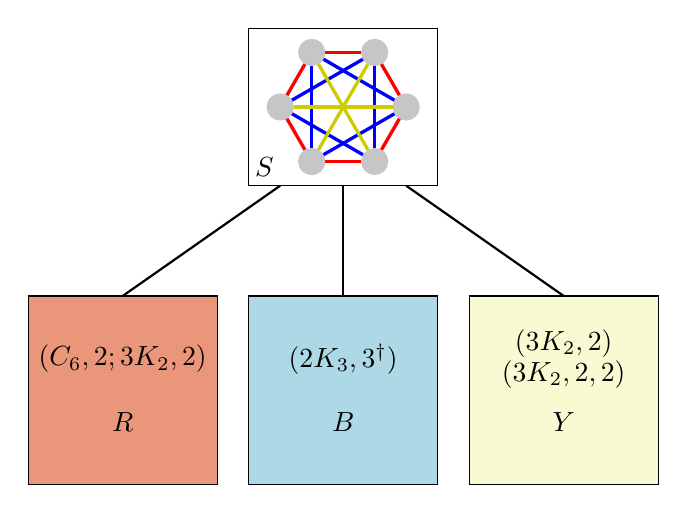
\begin{tikzpicture}[scale=0.8]
    \begin{scope}[shift = {(0,0)}]
        \draw[black] (-1.5,-1.25) rectangle ++(3,2.5);
        \node at (-1.25,-0.95) {$S$};
        \foreach \x in {0,...,5}
        {
            \node[vertex,lightgray,fill=lightgray] (p\x) at (\x*60+60:1) {};
        }
        \draw[edge,red] (p0) -- (p1);
        \draw[edge,red] (p1) -- (p2);
        \draw[edge,red] (p2) -- (p3);
        \draw[edge,red] (p3) -- (p4);
        \draw[edge,red] (p4) -- (p5);
        \draw[edge,red] (p5) -- (p0);

        \draw[edge,blue] (p0) -- (p2);
        \draw[edge,blue] (p2) -- (p4);
        \draw[edge,blue] (p4) -- (p0);
        \draw[edge,blue] (p1) -- (p3);
        \draw[edge,blue] (p3) -- (p5);
        \draw[edge,blue] (p5) -- (p1);

        \draw[edge,darkyellow] (p0) -- (p3);
        \draw[edge,darkyellow] (p1) -- (p4);
        \draw[edge,darkyellow] (p2) -- (p5);
    \end{scope}

    \begin{scope}[shift = {(-3.5,-4)}]
        \filldraw[draw=black,fill=lightred] (-1.5,-2) rectangle ++(3,3);
        \node at (0,-1) {$R$};
        \node at (0,0) {$\ipsixMatchingAndCycle$};
        \coordinate (largeRed) at (0,1) {};
    \end{scope}

    \begin{scope}[shift = {(0,-4)}]
        \filldraw[draw=black,fill=lightblue]   (-1.5,-2) rectangle ++(3,3);
        \node at (0,-1) {$B$};
        \node at (0,0) {$\ipsixTriangle$};
        \coordinate (largeBlue) at (0,1) {};
    \end{scope}

    \begin{scope}[shift = {(3.5,-4)}]
        \filldraw[draw=black,fill=lightyellow] (-1.5,-2) rectangle ++(3,3);
        \node at (0,-1) {$Y$};
        \node at (0,0.25) {$\ipsixMatching$};
        \node at (0,-0.25) {$\ipsixMatchingTwice$};
        \coordinate (largeYellow) at (0,1) {};
    \end{scope}
    \draw[edge,black,thick] (largeBlue) -- (0,-1.25);
    \draw[edge,black,thick] (largeRed) -- (-1,-1.25);
    \draw[edge,black,thick] (largeYellow) -- (1,-1.25);

\end{tikzpicture}
         \end{center}
        \subcaption{$|\ul(\inducedCC{S})| = 4$.}
        \label{restorable:6cc:monochormatic-cycle/fig}
    \end{subfigure}
    \hfill
    \begin{subfigure}[]{.4\textwidth}
        \begin{center}
            

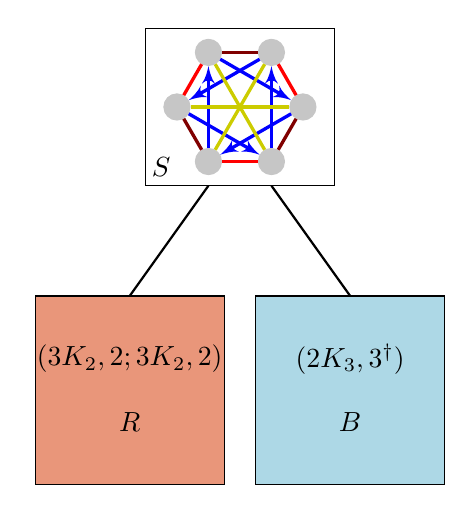
\begin{tikzpicture}[scale=0.8]

    \begin{scope}[shift = {(0,0)}]
        \draw[black] (-1.5,-1.25) rectangle ++(3,2.5);
        \node at (-1.25,-0.95) {$S$};
        \foreach \x in {0,...,5}
        {
            \node[vertex,lightgray,fill=lightgray] (p\x) at (\x*60+60:1) {};
        }
        \draw[edge,darkred] (p0) -- (p1);
        \draw[edge,red] (p1) -- (p2);
        \draw[edge,darkred] (p2) -- (p3);
        \draw[edge,red] (p3) -- (p4);
        \draw[edge,darkred] (p4) -- (p5);
        \draw[edge,red] (p5) -- (p0);

        \draw[arrow,blue] (p0) -- (p2);
        \draw[arrow,blue] (p2) -- (p4);
        \draw[arrow,blue] (p4) -- (p0);
        \draw[arrow,blue] (p1) -- (p5);
        \draw[arrow,blue] (p5) -- (p3);
        \draw[arrow,blue] (p3) -- (p1);

        \draw[edge,darkyellow] (p0) -- (p3);
        \draw[edge,darkyellow] (p1) -- (p4);
        \draw[edge,darkyellow] (p2) -- (p5);
    \end{scope}

    \begin{scope}[shift = {(-1.75,-4)}]
        \filldraw[draw=black,fill=lightred] (-1.5,-2) rectangle ++(3,3);
        \node at (0,-1) {$R$};
        \node at (0,0) {$\ipsixMatchingMatching$};
        \coordinate (largeRed) at (0,1) {};
    \end{scope}

    \begin{scope}[shift = {(1.75,-4)}]
        \filldraw[draw=black,fill=lightblue]   (-1.5,-2) rectangle ++(3,3);
        \node at (0,-1) {$B$};
        \node at (0,0) {$\ipsixTriangle$};
        \coordinate (largeBlue) at (0,1) {};
    \end{scope}

    \draw[edge,black,thick] (largeRed) -- (-0.5,-1.25);
    \draw[edge,black,thick] (largeBlue) -- (0.5,-1.25);

\end{tikzpicture}
         \end{center}
        \subcaption{$|\ul(\inducedCC{S})| = 5$.}
        \label{restorable:6cc:alternating-cycle/fig}
    \end{subfigure}
    \caption{Visualisation of the neighbor subset partition in Lemma~\ref{critical:6-cc:restorable:large-neighborhood/lem}.}
    \label{restorable:6cc/fig}
\end{figure}


\begin{lemma}
\label{critical:6-cc:restorable:large-neighborhood/lem}
    Let~$\coherentConfig$ be a critical coherent configuration and~$S \in \fibers{\coherentConfig}$ be a fiber such that~$\abs{S} = 6$, $\abs{\ul(\inducedCC{S})} > 3$, and~$\{S\}$ is not dominating.
    There exist disjoint subsets~$\mathcal{R},\mathcal{B}, \mathcal{Y}$ partitioning the neighborhood of~$S$ in~$\quotientGraph{\coherentConfig}$ with~$\mathcal{R},\mathcal{B}$ non-empty (and~$\mathcal{Y}$ possibly empty) such that
    \begin{enumerate}
        \item for all~$R \in \mathcal{R}$ the interspace~$\interspace{R}{S}$ has either interspace pattern~$\ipsixMatchingAndCycle$ or interspace pattern~$\ipsixMatchingMatching$,
        \item for all~$B \in \mathcal{B}$ the interspace~$\interspace{B}{S}$ has interspace pattern~$\ipsixTriangle$,
        \item for all~$Y \in \mathcal{Y}$ the interspace~$\interspace{Y}{S}$ has either interspace pattern~$\ipsixMatching$ or interspace pattern~$\ipsixMatchingTwice$.
    \end{enumerate}
    In particular, $\colorDeg{S} \geq 2$. (See Figure~\ref{restorable:6cc/fig})
\end{lemma}
\begin{proof}
    Let~$\mathcal{N}$ be the neighborhood of fiber~$S$ in~$\quotientGraph{\coherentConfig}$.
    Due to Lemma~\ref{small-cc:induced-cc/lem}, Corollary~\ref{large-small-interspace:classification:uniqueness/cor}, and~$\abs{\ul(\inducedCC{S})} > 3$, for all~$R \in \mathcal{N}$ the interspace~$\interspace{R}{S}$ has one of the following interspace patterns:
    $\ipsixMatchingAndCycle$, $\ipsixMatchingMatching$, $\ipsixMatching$, $\ipsixMatchingTwice$, or~$\ipsixTriangle$.
    Thus~$\mathcal{N}$ partitions into~$\{\mathcal{R},\mathcal{B}, \mathcal{Y}\}$ defined in the claim.
    Before we proof that~$S$ is restorable if~$\mathcal{R}$ or~$\mathcal{B}$ are empty, we first argue that by Lemma~\ref{critical:restorable:take-care/lem} we may assume the each part of~$\{\mathcal{R},\mathcal{B}, \mathcal{Y}\}$ has at most size~$1$.

    Assume that~$|\ul(\inducedCC{S})| = 4$.
    For all fibers~$R \in \mathcal{R}$ the interspace~$\interspace{R}{S}$ has interspace pattern~$\ipsixMatchingAndCycle$.
    By coherence there are the constituents in~$\inducedCC{S}$ isomorphic to~$\cycle{6}$, $\disjointCliques{3}{2}$, or~$\disjointCliques{2}{3}$, which by Lemma~\ref{small-cc:induced-cc/lem} are unique in~$S$.
    Hence for all~$\mathcal{F} \in \{\mathcal{R},\mathcal{B}, \mathcal{Y}\}$ the following holds:
    for all distinct~$F,F' \in \mathcal{F}$ the fiber~$F$ takes care of~$F'$ with regard to restorability of~$S$.
    Thus by Lemma~\ref{critical:restorable:take-care/lem} we may assume~$|\mathcal{F}| \leq 1$.
    Furthermore, if~$R \in \mathcal{R}$ exists, then~$R$ takes care of all~$Y \in \mathcal{Y}$, and thus by Lemma~\ref{critical:restorable:take-care/lem} we may assume~$\mathcal{Y} = \emptyset$ if~$|\mathcal{R}| = 1$.

    Assume that~$|\ul(\inducedCC{S})| = 5$.
    For all fibers~$R \in \mathcal{R}$ the interspace~$\interspace{R}{S}$ has interspace pattern~$\ipsixMatchingMatching$ and by coherence~$\mathcal{Y} = \emptyset$.
    In~$\ul(\inducedCC{S})$ the constituent isomorphic to~$\disjointCliques{2}{3}$ is unique, and thus by Lemma~\ref{critical:restorable:take-care/lem} we may assume~$|\mathcal{B}| \leq 1$.
    Further, since for all constituents~$G$ isomorphic to~$\disjointCliques{3}{2}$ there is a basis relation~$U \in \interspace{R}{S}$ such that for all~$r \in R$ the set~$rU$ induces a~$2$-clique in~$G$, for any distinct~$R,R' \in \mathcal{R}$ the fiber~$R$ takes care of~$R'$ with regard to restorability of~$S$.
    Thus by Lemma~\ref{critical:restorable:take-care/lem}, we may assume~$|\mathcal{R}| \leq 1$.

    In the following we show that~$S$ is restorable if~$\mathcal{R}$ or~$\mathcal{B}$ are empty.
    By the reasoning above, assume there are only fibers adjacent to~$S$ in~$\quotientGraph{\coherentConfig}$ which are not taken care of by some other fiber.
    Lemma~\ref{critical:6-cc:restorable:DUC:deg1/lem} implies that there are at least two fibers such that their interspaces have different patterns.
    Together with the reasoning above, we only have to consider the case in which~$\mathcal{R}$ is empty while~$|\mathcal{B}| = |\mathcal{Y}| = 1$.

    Let~$(Y,S,B)$ be a path in~$\quotientGraph{\coherentConfig}$ such that~$Y \in \mathcal{Y}$ and~$B \in \mathcal{B}$.
    Lemma~\ref{interspace-pattern:partition-structure/lem} determines~$\partitionStructure{B,S}$ and~$\partitionStructure{Y,S}$ as follows.
    While~$\partitionStructure{B,S}$ is isomorphic to~$K_2$, the isomorphism type of~$\partitionStructure{Y,S}$ is determined by isomorphism types of its constituents~$(3K_2,3K_2,2\overrightarrow{C_3},3K_2)$ or~$(K_3)$ or~$(\overrightarrow{C_3})$.
    Let~$\mathfrak{S}$ be the color-disjoint union of~$\partitionStructure{B,S}$ and~$\partitionStructure{Y,S}$.
    All automorphisms of~$\mathfrak{S}$ are induced by an automorphism of~$\inducedCC{S}$.
    Thus all automorphisms of~$\inducedCC{B \cup Y}$ extend to an automorphism of~$\inducedCC{B \cup Y \cup S}$.
\end{proof}


\begin{lemma}
    \label{critical:6-cc:restorable:cycle/lem}
    Let~$\coherentConfig$ be a critical coherent configuration and~$R,S \in \fibers{\coherentConfig}$ be distinct fibers of size~$6$ such that $\cycle{12} \in \interspace{R}{S}$ and~$\{R,S\}$ is not dominating.
    There exist disjoint, non-empty subsets~$\mathcal{B}, \mathcal{Y}$ of the neighborhood of~$S$ without~$R$ in~$\quotientGraph{\coherentConfig}$ such that
    \begin{enumerate}
        \item for all~$B \in \mathcal{B}$ the interspace~$\interspace{B}{S}$ has interspace pattern~$\ipsixTriangle$ and
        \item for all~$Y \in \mathcal{Y}$ the interspace~$\interspace{Y}{S}$ has either interspace pattern~$\ipsixMatching$ or interspace pattern~$\ipsixMatchingTwice$.
    \end{enumerate}
    In particular, $\colorDeg{S} \geq 3$.
\end{lemma}
\begin{proof}
    Lemma~\ref{critical:adjacent-interspace-cycle/lem} implies the uniqueness of~$R$ with respect to~$S$ and vice versa.
    Since~$\{R,S\}$ is not dominating, Lemma~\ref{critical:6-cc:restorable:large-neighborhood/lem} applies to both~$R$ and~$S$:
    hence for both~$R$ and~$S$ there is a fiber~$B$ such that~$\interspace{B}{S}$ (respectively~$\interspace{B}{R}$) has interspace pattern~$\ipsixTriangle$.
    Furthermore, we only need to consider~$\mathcal{Y} = \emptyset$.
    Recall that by Lemma~\ref{6-cc:implied-interspace:DUC-DUC/lem} for every fiber~$Y$ for which~$\interspace{Y}{R}$ has interspace pattern~$\ipsixMatching$ or~$\ipsixMatchingTwice$ the interspace~$\interspace{Y}{S}$ has interspace pattern~$\ipsixMatching$ or~$\ipsixMatchingTwice$ as well.
    Therefore, we only need to argue restorability in the following case, which will then contradict Lemma~\ref{critical:restorable/lem}:

    Let~$(B,R,S,B')$ be a possibly closed path in~$\quotientGraph{\coherentConfig}$ such that~$\cycle{12} \in \interspace{R}{S}$ and both~$\interspace{B}{R}$ and~$\interspace{B'}{S}$ have interspace pattern~$\ipsixTriangle$, and let~$U \in \interspace{R}{S}$.
    By arguments similar to the ones which appeared in the proof of Lemma~\ref{critical:6-cc:restorable:large-neighborhood/lem}, we may assume that~$B$ (respectively~$B'$) are unique regarding~$R$ (respectively~$R'$).
    If~$B \neq B'$, then let~$\mathfrak{S}$ be color-disjoint union of~$\partitionStructure{B,R}$ and~$\partitionStructure{B',S}$, both of which are isomorphic to~$K_2$.
    If~$B = B'$, then let~$\mathfrak{S}$ be~$\partitionStructure{B,R \cup S}$.
    If~$\equivalenceClasses{B,R} = \equivalenceClasses{B',S}$, then~$\mathfrak{S} \cong K_2$.
    If~$\equivalenceClasses{B,R} \neq \equivalenceClasses{B',S}$, then~$\equivalenceClasses{B,R}$ and~$\equivalenceClasses{B',S}$ are fully intersecting and the isomorphism type of~$\mathfrak{S}$ is determined by the isomorphism types of its constituents~$(2K_2,2K_2,2K_2)$.
    All automorphisms of~$\mathfrak{S}$ are induced by an automorphism of~$\inducedCC{S \cup R}$.
    Thus each automorphism of~$\inducedCC{B \cup B'}$ extends to an automorphism of~$\inducedCC{B \cup R \cup S \cup B'}$.
    Overall~$\{R,S\}$ is not dominating, but~$R \cup S$ is restorable.
\end{proof}


Next we deal with interspaces isomorphic to~$\interspaceFourSix \in \interspace{R}{B}$ for fibers~$R,B$ with~$|R| < |B|$.
Such an interspace has a different pattern depending on the perspective.
Interspace~$\interspace{R}{B}$ has interspace pattern~$\ipsixMatchingComplementD$, while interspace~$\interspace{B}{R}$ has interspace pattern~$\ipfourClique$.


\begin{lemma}
\label{critical:4cc-6cc/lem}
    Let~$\coherentConfig$ be critical coherent configuration, and let~$R,S \in \fibers{\coherentConfig}$ fibers such that~$\interspace{R}{S}$ has interspace pattern~$\ipsixMatchingComplementD$.
    \begin{enumerate}
        \item\label{4cc-6cc:part1}
        If~$\colorDeg{R} = 1$, then~$\{S\}$ is dominating and for all fibers~$Y$ adjacent to~$S$ in~$\quotientGraph{\coherentConfig}$ other than~$R$ the interspace~$\interspace{Y}{S}$ has either interspace pattern~$\ipsixMatching$ or interspace pattern~$\ipsixMatchingTwice$.
        \item
        If~$\interspaceFourSix \in \interspace{R}{S}$ and all fibers of~$\coherentConfig$ are small, then~$\wldim{\coherentConfig} = 2$.
    \end{enumerate}
\end{lemma}
\begin{proof}
    We begin by proving the first statement.
    Set~$U = U^1_1(\interspace{R}{S})$.
    Due to the interspace pattern of~$\interspace{R}{S}$, we have either~$\clique{2,2,2} \in \inducedCC{S}$ or~$\overrightarrow{C_3}[K_2] \in \inducedCC{S}$.
    Thus by Lemma~\ref{small-cc:induced-cc/lem} we have~$\disjointCliques{3}{2} \in \inducedCC{S}$.
    Hence~$|\ul(\inducedCC{S})| = 3$.

    Next we show that all interspaces incident to~$S$ in~$\quotientGraph{\coherentConfig}$ have either interspace pattern~$\ipsixMatching$ or interspace pattern~$\ipsixMatchingTwice$.
    Towards a contradiction, suppose that there is a fiber~$Y$ adjacent to~$S$ in~$\quotientGraph{\coherentConfig}$ other than~$R$ such that~$\interspace{Y}{S}$ has an interspace pattern other than~$\ipsixMatching$ or~$\ipsixMatchingTwice$.
    So~$\interspace{Y}{S}$ has interspace pattern~$\ipsixMatchingComplement$ or~$\ipsixMatchingComplementD$.
    Let~$U' = U^1_1(\interspace{Y}{S})$.
    For all~$P \in \equivalenceClasses{Y,S}$ there is exactly one~$Q\in \equivalenceClasses{R,S}$ such that for all~$p \in P,q\in Q$ we have either~$p U = q U'$ or~$p U \cap q U' = \emptyset$.
    Thus interspace~$\interspace{Y}{R}$ is not homogeneous, which contradicts~$\colorDeg{R} = 1$.

    Before we show that the set~$R \cup S$ is restorable, we argue that by Lemma~\ref{critical:restorable:take-care/lem} we may assume~$\colorDeg{S} = 2$.
    Let~$\mathcal{Y}$ the set of all fibers adjacent to~$B$ other than~$R$.
    By the previous reasoning for all~$Y \in \mathcal{Y}$ the interspace~$\interspace{Y}{S}$ has interspace pattern~$\ipsixMatching$ or~$\ipsixMatchingTwice$.
    Since~$|\ul(\inducedCC{B})| = 3$, there is~$Y \in \mathcal{Y}$ which takes care of all~$Y' \in \mathcal{Y}$ (other than~$Y$).
    Hence we may assume that~$\mathcal{Y} = \{Y\}$ and~$\colorDeg{S} = 2$.

    Lemma~\ref{interspace-pattern:partition-structure/lem} determines the partition structure of~$\interspace{R}{S}$ and~$\interspace{Y}{S}$ as follows.
    While~$\partitionStructure{R,S}$ is isomorphic to~$K_4$, either~$\partitionStructure{Y,S} \cong K_3$ or the isomorphism type of~$\partitionStructure{Y,S}$ is determined by isomorphism types of its constituents~$(3K_2,3K_2,2\overrightarrow{C_3},3K_2)$.
    All automorphisms of~$\partitionStructure{Y,S}$ are induced by an automorphism of~$\inducedCC{S}$ and that all automorphisms of~$\inducedCC{S}$ are induced by an automorphism of~$\partitionStructure{R,S}$.
    Thus all automorphisms of~$\inducedCC{Y}$ extend to an automorphism of~$\inducedCC{Y \cup S \cup R}$, and hence~$R \cup B$ is restorable.
    By Lemma~\ref{critical:restorable/lem} the set~$\{R,S\}$ is not dominating.
    Since~$\colorDeg{R} = 1$, we conclude that~$\{S\}$ is dominating.

We now prove the second statement with the help of the first.
    So let~$R,S$ be fibers of~$\coherentConfig$ such that~$\interspaceFourSix \in \interspace{R}{S}$.
    Observe that~$\interspace{S}{R}$ has interspace pattern~$\ipsixMatchingComplementD$.
    Set~$U = U^1_1(\interspace{R}{S})$.
    To apply the first statement to this situation, it remains to argue that~$\colorDeg{R} = 1$.
    By Lemma~\ref{small-cc:interspace-implies-cc/lem} we have~$\clique{4} \in \inducedCC{R}$.
    Towards a contradiction, suppose~$\colorDeg{R} > 1$ and thus there is a fiber~$B$ other than~$R$ such that~$\interspace{B}{R}$ has interspace pattern~$\ipfourClique$.
    Let~$U' = U^1_1(\interspace{B}{R})$.
    For all~$s \in S$ there is exactly one~$P \in \equivalenceClasses{B,R}$ such that for all~$p \in P$ we have~$pU' = sU^\star$.
    Hence~$\disjointCliques{6}{\frac{\abs{B}}{6},1} \in \interspace{B}{S}$.
    This violates Lemma~\ref{critical:star/lem}.

    Let~$\mathcal{Y}$ be the set of fibers adjacent to~$S$ other than~$R$.
    By assumption all~$Y \in \mathcal{Y}$ are small.
    By the first part of the Lemma, we conclude~$\{S\}$ is dominating and for all fibers~$Y \in \mathcal{Y}$ we have~$\disjointCliques{3}{2,2} \in \interspace{Y}{S}$.
    Thus for all distinct~$Y,Y' \in \mathcal{Y}$ Lemma~\ref{6-cc:implied-interspace:DUC-DUC/lem} implies~$\disjointCliques{3}{2,2} \in \interspace{Y}{Y'}$.
    Note that for all~$Y \in \mathcal{Y}$ the interspace~$\interspace{Y}{R}$ is homogeneous.
    Therefore for all~$Y \in \mathcal{Y}$ there is no interspace incident to~$Y$ in~$\quotientGraph{\coherentConfig}$ containing a constituent isomorphic to~$\disjointCliques{2}{3,3}$.
    Furthermore, there are no dominating fibers in~$\mathcal{Y}$.
    Lemma~\ref{critical:6-cc:restorable:cycle/lem} implies that~$\cycle{12} \notin \interspace{Y}{Y'}$ for all~$Y,Y' \in \mathcal{Y}$.
    By Lemma~\ref{critical:6-cc:restorable:DUC:deg1/lem} we have~$\mathcal{Y} = \emptyset$ and~$\vertices(\coherentConfig) = R \cup S$.
    Recall that~\wltwo identifies cliques, and complements of matchings.
    Furthermore on small fibers, the set of constituent graphs defines the coherent configuration.
    Since~$\abs{r U \cap r' U} = 1$ for all distinct~$rr' \in R^2$, \wltwo distinguishes~$\interspaceFourSix$ from~$\disjointCliques{2}{2,3}$.
    This yields~$\wldim{\coherentConfig} = 2$.
\end{proof}


\begin{lemma}
\label{critical:7-cc:leviFano/lem}
    If~$\coherentConfig$ is a critical coherent configuration, then there is no path~$(R,B,Y)$ in~$\quotientGraph{\coherentConfig}$ such that~$\leviFano \in \interspace{R}{B}$ and~$\leviFano \in \interspace{B}{Y}$.
\end{lemma}
\begin{proof}
    Towards a contradiction, suppose that such a path exists.
    Let~$U \in \interspace{R}{B}$ and~$U' \in \interspace{Y}{B}$ be such that~$(R \disjointUnion B, U) \cong \leviFano$ and~$(Y \disjointUnion B, U') \cong \leviFano$.
    Suppose~$r \in R$.
    \begin{itemize}
        \item
        If there is~$y \in Y$ such that~$\abs{r U \cap y U'} = 3$, then~$\matching{7} \in \interspace{R}{Y}$ due to Property~\ref{coherent-config:wl2}.

        \item
        Assume there is~$y \in Y$ such that~$\abs{r U \cap y U'} \in \{1,2\}$ and~$Y = \{y_1, \dots, y_7\}$.
        Without loss of generality, assume for all~$i \in \{1,2,3\}$ we have~$\abs{r U \cap y_i U'} = 2$, for all~$i \in \{4,5,6\}$ we have~$\abs{r U \cap y_i U'} = 1$.
        Hence~$\abs{r U \cap y_7 U'} = 0$ and~$\matching{7} \in \interspace{R}{Y}$.

        \item
        Assume there is~$y \in Y$ such that~$\abs{r U \cap y U'} = 0$.
        Suppose that there is~$y' \in  Y \setminus \{y\}$ such that~$\abs{r U \cap y' U'} = 0$.
        Thus there are~$\{b,b'\} \subset B \setminus r U$ such that~$\abs{b U'^\star \cap b' U'^\star} = 2$.
        Since this violates the properties of~$\leviFano$, we have~$\matching{7} \in \interspace{R}{Y}$.
    \end{itemize}
    By Lemma~\ref{critical:star/lem}, the coherent configuration~$\coherentConfig$ is not critical in any of these cases.
\end{proof}


\begin{lemma}
\label{restorable:two-3K2,2-ip:fully-intersecting/lem}
    Let~$\coherentConfig$ be a critical coherent configuration and~$(S,L,S')$ be a path in~$\quotientGraph{\coherentConfig}$ such that~$\interspace{L}{S}$ and~$\interspace{L}{S'}$ both have interspace pattern~$\ipsixMatching$.
    If~$|L| = 9$, $\colorDeg{L} = 2$, $|\ul(\inducedCC{L})| = 4$, and~$\equivalenceClasses{L,S}$ and~$\equivalenceClasses{L,S'}$ are fully intersecting, then~$\{L\}$ is dominating.
\end{lemma}
\begin{proof}
    Let~$S_0,S_1,S_2$ and~$S'_0,S'_1,S'_2$ be the $3$-cliques in~$(S,\arcs^1(\interspace{L}{S}))$ and~$(S',\arcs^1(\interspace{L}{S'}))$ respectively.
    Let~$U  = U^1_1(\interspace{L}{S})$ and~$U' = U^1_1(\interspace{L}{S'})$.
    To write the proof in a concise manner, we rename the vertices of~$L$ as follows.
    Assume that~$L = \{\ell^r_c \mid r,c \in \{0,1,2\}\}$.
    Further, assume that~$\ell^r_c U = S_c$ and~$\ell^r_c U' = S'_r$ for all~$r,c \in \{0,1,2\}$.
    Let~$\psi$ be an automorphism of~$\inducedCC{S \cup S'}$.
    Due to the interspace pattern of~$\interspace{L}{S}$ and~$\interspace{L}{S'}$, we are only interested in the permutation of~$\{S_0,S_1,S_2\}$ and~$\{S'_0,S'_1,S'_2\}$.
    Thus, let~$\psi'$ be the permutation of~$\{S_0,S_1,S_2\}$ and~$\{S'_0,S'_1,S'_2\}$ induced by~$\psi$, let~$\pi$ be projection mapping~$S_r$ to~$r$, and~$\mu$ be the projection of~$S'_c$ to~$c$.
    We now define~$\varphi$ be an automorphism on~$L \cup S$:
    \[
        \varphi(v) \coloneqq
        \begin{cases}
            \ell^{(\pi \circ \psi' \circ \reverseFunction{\pi})(r)}_{(\mu \circ \psi' \circ \reverseFunction{\mu})(c)}, &\text{if } v = \ell^r_c, \\
            \psi(v),                                                                                                    &\text{if } v \in S \cup S'.
        \end{cases}
    \]
    Thus~$\varphi$ is a extension of~$\psi$ and~$L$ is restorable.
    Therefore by Lemma~\ref{critical:restorable/lem} the set~$\{L\}$ is dominating.
\end{proof}




 


\section{Weisfeiler-Leman dimension of graphs with small fibers}
\label{wldim-small/sec}


\begin{theorem}
    \label{critical:small-cc/thm}
    Let~$\coherentConfig$ be a critical coherent configuration.
    If all fibers of~$\coherentConfig$ are small, then either
    \begin{enumerate}
        \item all fibers have the same size, or
        \item for all~$R \in \fibers{\coherentConfig}$ we have~$\abs{R} \in \{4,6\}$.
    \end{enumerate}
\end{theorem}
\begin{proof}
    This follows directly from Lemmas~\ref{critical:disjoint-union/lem} and~\ref{small-cc:interspace/lem}.
\end{proof}


\begin{lemma}
\label{4-cc:cdeg-decrease/lem}
    Let~$\coherentConfig$ be a critical coherent configuration such that all fibers of~$\coherentConfig$ have size~$4$.
    A fiber~$R$ of~$\coherentConfig$ and all fibers adjacent to it in~$\quotientGraph{\coherentConfig}$ split entirely into tiny fibers in~$\coherentConfig_r$ where~$r \in R$.

    In particular, if~$\colorDeg{R} \geq 4$, then~$\wldim{\coherentConfig}=2$ or  there is a critical coherent configuration~$\coherentConfig'$ for which $\wldim{\coherentConfig} \leq  1 + \wldim{\coherentConfig_r} = 1 + \wldim{\coherentConfig'}$ with~$\abs{\vertices(\coherentConfig)} \leq \abs{\vertices(\coherentConfig')} - 20$.
\end{lemma}
\begin{proof}
    Let~$r \in R$ and~$\{B_1, \dots, B_{\colorDeg{R}}\}$ be the neighborhood of~$R$ in~$\quotientGraph{\coherentConfig}$.
    Since~$|R| = 4$, fiber~$R$ splits into tiny fibers in~$\coherentConfig_r$.
    By Lemma~\ref{small-cc:interspace/lem}, all interspaces incident to~$R$ in~$\quotientGraph{\coherentConfig}$ contain a constituent isomorphic to~$\cycle{8}$ or~$\disjointCliques{2}{2,2}$.
    Hence in~$\coherentConfig_r$ all fibers adjacent to~$R$ in~$\quotientGraph{\coherentConfig}$ split in half.
    This means~$\coherentConfig_r- \{R,B_1,\ldots,B_{\colorDeg{R}}\}$ has WL-dimension at least~$\wldim{\coherentConfig}-1$.
    If~$\wldim{\coherentConfig}>2$, we obtain a critical coherent configuration~$\coherentConfig'$ such that~$\vertices(\coherentConfig') \subseteq \vertices(\coherentConfig) \setminus (R \cup \bigcup_{i=1}^{\colorDeg{R}}B_i)$.
    Observe that~$|R \cup \bigcup_{i=1}^{\colorDeg{R}} B_i| \geq 20$.
\end{proof}


The lemma essentially allows us to reduce the degree of the quotient graph. For graphs with maximum degree at most~$3$, we can make use of a bound by Fomin and H{\o}ie on the pathwidth of the graph.


\begin{theorem}[see \cite{pathwidthCubicGraphs}]
\label{tw-cubic-graph/lem}
    For every $\epsilon > 0$, there exists $n_0 \in \Nat$ such that every graph of maximum degree at most~$3$ with at at least~$n$ vertices satisfies $\treewidth(G)\leq \pathwidth(G) \leq \frac{n}{6} + \epsilon$.
\end{theorem}


We use the theorem to bound the Weisfeiler-Leman dimension for certain graphs as follows.


\begin{theorem}
\label{4-cc:cfi-wldim/thm}
    Let~$\coherentConfig$ be a critical coherent configuration on~$n$ vertices such that all fibers of~$\coherentConfig$ have size~$4$ and there is no interspace containing a constituent isomorphic to~$\cycle{8}$.
    If all fibers of~$\coherentConfig$ have at most~$3$ neighbors in~$\quotientGraph{\coherentConfig}$, then~$\wldim{\coherentConfig} \leq \frac{n}{24} + \mathcal{O}(1)$.
\end{theorem}
\begin{proof}[Proof Sketch]
    If there is a dominating fiber~$R$ for which~$\colorDeg{R} \leq 3$, then~$n\leq 16$.
    Thus $\wldim{\coherentConfig} \leq 3$.
    So assume there is no dominating fiber in~$\coherentConfig$.
    Since there are no interspace containing constituents isomorphic to~$\cycle{8}$, Lemma~\ref{critical:4cc:restorable:2,C4/lem} implies~$|\ul(\inducedCC{R})| = 4$ for all~$R \in \fibers{\coherentConfig}$.
    By Lemma~\ref{critical:4-cc:restorable:DUC/lem}, the quotient graph~$\quotientGraph{\coherentConfig}$ is~$3$-regular.
    Furthermore, whenever we individualize a vertex~$r$ in a fiber~$R$, $R$ splits into singletons in~$\coherentConfig_r$.

    By Lemma~\ref{tw-cubic-graph/lem} we have~$\treewidth(\quotientGraph{\coherentConfig}) \leq \frac{\abs{\fibers{\coherentConfig}}}{6} + \varepsilon$ for constant ~$\varepsilon > 0$.
    Let~$\coherentConfig'$ be another coherent configuration satisfying the same assumptions.
    Thus in the cops and robbers game played on the quotient graphs~$\quotientGraph{\coherentConfig}$ and~$\quotientGraph{\coherentConfig'}$ there is a winning strategy for~$t$ cops, where~$t \leq \frac{n}{6} + \varepsilon$.
    We mimic this winning strategy now on the corresponding coherent configurations~$\coherentConfig$ and~$\coherentConfig'$ in the bijective pebble game as follows (see e.g.~\cite{DBLP:conf/swat/OtachiS14} for more information on the connection between the two games).
    Whenever we place a pebble on fiber~$R$ in~$\quotientGraph{\coherentConfig}$ (respectively~$\quotientGraph{\coherentConfig'}$) we now place the corresponding pebble on some vertex~$r$ of the corresponding fiber~$R$ in~$\coherentConfig$ (respectively~$\coherentConfig'$).
    By the reasoning above this fiber splits into singletons after applying the coherent closure.
    Therefore, Spoiler has a winning strategy if we add two additional pebbles to the game.

    We conclude~$\wldim{\coherentConfig} \leq \frac{\abs{\fibers{\coherentConfig}}}{6} + 2 + \varepsilon \leq \frac{n}{24} + 2 + \varepsilon$.
\end{proof}


\begin{corollary}
\label{4-cc:wldim/cor}
    Let~$\coherentConfig$ be a critical coherent configuration on~$n$ vertices such that all fibers of~$\coherentConfig$ have size~$4$.
    Then~$\wldim{\coherentConfig} \leq \frac{n}{20} + \mathcal{O}(1)$.
\end{corollary}
\begin{proof}
    First, we apply Lemma~\ref{4-cc:cdeg-decrease/lem} repeatedly and restore the criticality after each application until the preconditions of Lemma~\ref{4-cc:cdeg-decrease/lem} are no longer satisfied. Say this happens~$k$ times.
    We then have a critical coherent configuration~$\coherentConfig'$ with~$\wldim{\coherentConfig} \leq k + \wldim{\coherentConfig}$ and whose quotient graph~$\quotientGraph{\coherentConfig'}$ has maximum degree~$3$.
    Observe that~$\abs{\vertices(\coherentConfig')} \leq n - 20 \cdot k$. Note that in the proof Lemma~\ref{4-cc:cdeg-decrease/lem} we repeatedly take the coherent closure after individualizations and restore criticality, thus all fibers of $\coherentConfig'$ have size exactly~$4$.

    If there are distinct fibers~$R,R'$ in~$\coherentConfig'$ such that~$\cycle{8} \in \interspace{R}{R'}$, then by Lemma~\ref{critical:4cc:restorable:cycle/lem} the set~$\{R,R'\}$ is dominating.
    Thus~$\abs{\vertices(\coherentConfig')} \leq 24$ and~$\wldim{\coherentConfig'} \leq 4\in O(1)$.

    Now assume there is no interspace in~$\coherentConfig'$ containing a constituent isomorphic to~$\cycle{8}$.
    Then we apply Theorem~\ref{4-cc:cfi-wldim/thm} and obtain~$\wldim{\coherentConfig'} \leq \frac{\abs{\vertices(\coherentConfig')}}{24} + \mathcal{O}(1)$.
    Altogether we have
    \[
        \wldim{\coherentConfig} \leq 2+k + \max \{4, \wldim{\coherentConfig'}\} \leq 2 + k + \max\{ 4, \frac{n - 20 \cdot k}{24} + \mathcal{O}(1)\}.
    \]
    Observe that~$k \leq \left\lceil \frac{n}{20} \right\rceil$. Thus~$\wldim{\coherentConfig} \leq \frac{n}{20} + \mathcal{O}(1)$.
\end{proof}


\begin{lemma}
\label{5-cc:wldim/lem}
    Let~$\coherentConfig$ be a critical coherent configuration such that all fibers of~$\coherentConfig$ have size~$5$.
    Then~$\abs{\fibers{\coherentConfig}} = 1$ and~$\wldim{\coherentConfig} \leq 2$.
\end{lemma}
\begin{proof}
    By Lemmas~\ref{critical:cycle/lem} and~\ref{small-cc:interspace/lem}, there is only one fiber~$R$ in~$\coherentConfig$.
    By Lemma~\ref{small-cc:induced-cc/lem}, either~$\clique{5} \in \inducedCC{R}$ or~$\cycle{5} \in \inducedCC{R}$.
    Thus~$\wldim{\coherentConfig} \leq 2$.
\end{proof}


\begin{lemma}
\label{6-cc:wldim/lem}
    If~$\coherentConfig$ is a critical coherent configuration whose fibers each have size~$4$ or~$6$, then $\wldim{\coherentConfig} \leq \frac{n}{20}+ \mathcal{O}(1)$.
\end{lemma}
\begin{proof}
    If there is an interspace in~$\coherentConfig$ containing the constituent~$\interspaceFourSix$, then by Lemma~\ref{critical:4cc-6cc/lem} we have~$\wldim{\coherentConfig} = 2$.
    If~$|\fibers{\coherentConfig}| = 1$, then we also have~$\wldim{\coherentConfig} \leq 2$.

    Let~$S \in \fibers{\coherentConfig}$ with~$\abs{S} = 6$ be incident to a non-homogeneous interspace in~$\quotientGraph{\coherentConfig}$, and let~$s \in S$.
    Thus by Lemmas~\ref{small-cc:interspace/lem} and~\ref{small-cc:interspace-implies-cc/lem} this yields~$\clique{6} \notin \inducedCC{S}$.
    By Lemma~\ref{small-cc:induced-cc/lem} we have~$\abs{\ul(\inducedCC{S})} \geq 3$.

    Assume that there are fibers~$F,F'$ such that the set~$\{F,F'\}$ is dominating.
    Since~$\abs{\ul(\inducedCC{F})} \geq 3$ and~$\abs{\ul(\inducedCC{F'})} \geq 3$, both fibers~$F$ and~$F'$ split into singletons if we individualize~$8$ carefully chosen vertices in~$F \cup F'$.
    Therefore all fibers adjacent to~$F$ or~$F'$ split into tiny fibers.
    Thus~$\wldim{\coherentConfig} \leq 8 + 2 \in \mathcal{O}(1)$.

    We may thus assume for the rest of the proof that there is are no distinct fibers~$F,F'$ in~$\coherentConfig$ such that~$\{F,F'\}$ is dominating.

    Assume that~$\abs{\ul(\inducedCC{S})} = 3$.
    By Lemma~\ref{small-cc:induced-cc/lem}, the configuration~$\inducedCC{S}$ contains two constituents whose underlying graphs are isomorphic either to~$\disjointCliques{3}{2}$ and~$\clique{2,2,2}$, respectively, or to~$\disjointCliques{2}{3}$ and~$\clique{3,3}$, respectively.
    Since all fibers are small, by Lemma~\ref{small-cc:interspace-implies-cc/lem} all interspaces incident to~$S$ in~$\quotientGraph{\coherentConfig}$ contain a constituent isomorphic to~$\disjointCliques{3}{2,2}$ but none isomorphic to~$\cycle{12}$ in the first case and one isomorphic to~$\disjointCliques{2}{3,3}$ in the second case.
    Since~$\{S\}$ is not dominating by assumption, this contradicts Lemma~\ref{critical:6-cc:restorable:DUC:deg1/lem}, and hence~$\abs{\ul(\inducedCC{S})} > 3$.

    Assume that~$\abs{\ul(\inducedCC{S})} = 5$.
    By Lemma~\ref{small-cc:induced-cc/lem} there are the following constituents in~$\inducedCC{S}$: three graphs isomorphic to~$\disjointCliques{3}{2}$ and two isomorphic to~$2\overrightarrow{C_3}$.
    By Lemma~\ref{small-cc:interspace-implies-cc/lem} there is no interspace incident to~$S$ in~$\quotientGraph{\coherentConfig}$ that contains a constituent isomorphic to~$\cycle{12}$.
    By Lemma~\ref{critical:6-cc:restorable:large-neighborhood/lem} there is a small fiber~$R$ adjacent to~$S$ such that~$\interspace{R}{S}$ has interspace pattern~$\ipsixMatchingMatching$.
    Thus~$\interspace{S}{R}$ has interspace pattern~$\ipsixMatchingTwice$.
    If~$|\ul(\inducedCC{R})| = 3$, then either~$\disjointCliques{3}{2},\clique{2,2,2} \in \inducedCC{R}$ or~~$\disjointCliques{3}{2},\overrightarrow{C_3}[K_2] \in \inducedCC{R}$.
    Therefore for all fibers~$R'$ adjacent to~$R$ in~$\quotientGraph{\coherentConfig}$ the interspace~$\interspace{R'}{R}$ has interspace pattern~$\ipsixMatching$ or~$\ipsixMatchingTwice$.
    Since~$\{S\}$ is not dominating, this contradicts Lemma~\ref{critical:6-cc:restorable:DUC:deg1/lem}.
    So~$|\ul(\inducedCC{R})| > 3$.
    Thus Lemma~\ref{critical:6-cc:restorable:large-neighborhood/lem} applies and the neighborhood of~$B'$ partitions into~$\{\mathcal{R},\mathcal{Y},\mathcal{B}\}$ with the properties as described in Lemma~\ref{critical:6-cc:restorable:large-neighborhood/lem}.
    Since~$S \in \mathcal{Y}$ (follows from interspace pattern of~$\interspace{S}{R}$), none of parts of~$\{\mathcal{R},\mathcal{Y},\mathcal{B}\}$ are empty.
    Let~$R' \in \mathcal{R}$ and~$B' \in \mathcal{B}$.
    Consider~$\coherentConfig_r$ where~$r \in R$.
    Then fibers~$R'$, $B'$, $R$, and~$S$ split into tiny fibers in~$\coherentConfig_r$.
    After restoring criticality, we obtain a critical coherent configuration~$\coherentConfig'$ such that~$\vertices(\coherentConfig') \subseteq \vertices(\coherentConfig) \setminus (R' \cup S \cup B' \cup Y)$.
    Note that~$\abs{\vertices(\coherentConfig')} \leq \abs{\vertices(\coherentConfig)} - 20$ since~$\abs{B} \in \{4,6\}$.

    Assume that~$|\ul(\inducedCC{S})| = 4$.
    By Lemma~\ref{small-cc:induced-cc/lem}, there is exactly one constituent in~$\inducedCC{S}$ which is isomorphic to~$\disjointCliques{3}{2}$.
    Hence there is no interspace incident to~$S$ which has interspace pattern~$\ipsixMatchingMatching$.
    Lemma~\ref{critical:6-cc:restorable:large-neighborhood/lem} applies, and therefore the neighborhood of~$S$ in~$\quotientGraph{\coherentConfig}$ partitions in~$\{\mathcal{R},\mathcal{B},\mathcal{Y}\}$ such that
    \begin{itemize}
        \item
        for all~$R \in \mathcal{R}$ we have~$\cycle{12} \in \interspace{S}{R}$,
        \item
        for all~$B \in \mathcal{B}$ we have~$\disjointCliques{2}{3,\frac{\abs{B}}{2}} \in \interspace{S}{B}$, and
        \item
        for all~$Y \in \mathcal{Y}$ the number of constituents in~$\interspace{S}{Y}$ isomorphic to~$\disjointCliques{3}{2,2}$ is exactly~1 or~3.
    \end{itemize}
    By Lemma~\ref{critical:6-cc:restorable:cycle/lem}, all sets~$\mathcal{R}, \mathcal{B}, \mathcal{Y}$ are non-empty and~$\mathcal{R}$ contains a single fiber unique to~$S$.
    Thus let~$R\in\mathcal{R}$, $B \in \mathcal{B}$, and~$Y \in \mathcal{Y}$.
    Now we have two cases:

    If there are exactly three constituents in~$\interspace{S}{Y}$ which are isomorphic to~$\disjointCliques{3}{2,2}$, then fibers~$R$, $B$, $Y$, and~$S$ split into tiny fibers in~$\coherentConfig_s$.
    After restoring criticality, we obtain a critical coherent configuration~$\coherentConfig'$ such that~$\vertices(\coherentConfig') \subseteq \vertices(\coherentConfig) \setminus (R \cup S \cup B \cup Y)$.
    Further note that~$\abs{\vertices(\coherentConfig')} \leq \abs{\vertices(\coherentConfig)} - 20$ since~$\abs{B} \in \{4,6\}$.

    Now assume that there is exactly one constituent in~$\interspace{S}{Y}$ which is isomorphic to~$\disjointCliques{3}{2,2}$.
    This implies~$|\ul(\inducedCC{Y})| \leq 4$.
    By Lemma~\ref{critical:small-cc:module/lem} we conclude that~$|\ul(\inducedCC{Y})| = 4$.
    Therefore there is no fiber~$R'$ adjacent to~$Y$ such that~$\interspace{R'}{Y}$ has interspace pattern~$\ipsixMatchingMatching$.
    Hence, Lemmas~\ref{critical:6-cc:restorable:large-neighborhood/lem} and additionally Lemma~\ref{critical:6-cc:restorable:cycle/lem} apply to~$Y$ since (otherwise we obtain a contradiction by reasoning similar to the one above; either~$\{Y\}$ would be dominating or~$|\ul(\inducedCC{Y})|=3$).
    Thus there is an~$F \in \fibers{\coherentConfig}$ such that~$\cycle{12} \in \interspace{Y}{F}$.
    Since~$\coherentConfig$ is critical, Lemma~\ref{critical:adjacent-interspace-cycle/lem} implies~$F \neq S$ and~$F \neq R$.
    Lemma~\ref{6-cc:implied-interspace:DUC-DUC/lem} implies~$\disjointCliques{3}{2,2} \in \interspace{S}{F}$.
    Observe that it is impossible in a critical coherent configuration for an interspace to contain both a constituent isomorphic to~$\disjointCliques{2}{3,3}$ and a constituent isomorphic to~$\disjointCliques{3}{2,2}$ (compare Table~\ref{small-cc:classificaiton-small-interspaces/tab}).
    Thus~$F \neq B$ and~$|\mathcal{Y}| \geq 2$.
    In~$\coherentConfig_s$ fibers~$R$, $S$, and~$B$ split into tiny fibers while size-$2$ fibers~$Y'$ and~$F'$ are split off from~$Y$ and~$F$, respectively.
    After we restore criticality, we obtain a critical coherent configuration~$\coherentConfig'$ such that~$\vertices(\coherentConfig') \subseteq \vertices(\coherentConfig) \setminus (R \cup Y' \cup S \cup B \cup F')$.
    Further note that~$\abs{\vertices(\coherentConfig')} = \abs{\vertices(\coherentConfig)} - 20$ since~$\abs{B} \in \{4,6\}$.

    We summarize the proof up to this point:
    in several edge cases, we have~$\wldim{\coherentConfig} \in \mathcal{O}(1)$.
    Since~$\coherentConfig$ is critical, there is no size-$6$ fiber with~$\abs{\ul(\inducedCC{S})} = 3$.
    If there is a size-$6$ fiber with~$\abs{\ul(\inducedCC{S})} > 3$, then $\wldim{\coherentConfig} \leq   1 + \wldim{\coherentConfig'}$ for a critical coherent configuration with~$\abs{\vertices(\coherentConfig')} \leq \abs{\vertices(\coherentConfig)} - 20$ also satisfying the assumptions of the lemma.

    We iterate the process above until no fiber of size~$6$ exits any more and define~$k$ to be the number of iterations.
    What remains is a coherent configuration~$\coherentConfig''$ whose fibers all have size~$4$.
    Thus we apply Corollary~\ref{4-cc:wldim/cor}.
    Altogether we have
    \[
        \wldim{\coherentConfig} \leq 2+ k + \max \{8, \wldim{\coherentConfig''}\} \leq 2 + k + \max\{8, \frac{n - 20 \cdot k}{20} + \mathcal{O}(1)\}.
    \]
    Observe that~$k \leq \left\lceil \frac{n}{20} \right\rceil$.
    We conclude~$\wldim{\coherentConfig} \leq \frac{n}{20} + \mathcal{O}(1)$.
\end{proof}


\begin{lemma}
\label{7-cc:wldim/lem}
    Let~$\coherentConfig$ be a critical coherent configuration such that all fibers of~$\coherentConfig$ have size~$7$.
    Then~$\abs{\fibers{\coherentConfig}} \leq 2$ and~$\wldim{\coherentConfig} \leq 3$.
\end{lemma}

\begin{proof}
    By Lemmas~\ref{critical:cycle/lem} and~\ref{critical:7-cc:leviFano/lem}, we have~$\abs{\fibers{\coherentConfig}} \in\{1,2\}$:
    assuming~$\fibers{\coherentConfig} = \{R\}$, then by Lemma~\ref{small-cc:induced-cc/lem} there is constituent in~$\inducedCC{R}$ whose underlying graph is isomorphic to~$\clique{7}$ or~$\cycle{7}$.
    Hence~$\wldim{\coherentConfig} \leq 2$.
    So we assume that~$\{R,B\} = \fibers{\coherentConfig}$ and~$U \in \interspace{R}{B}$ such that~$(R \disjointUnion B, U) \cong \leviFano$.
    By Lemma~\ref{small-cc:induced-cc/lem} we have~$\clique{7} \in \inducedCC{R}$ and~$\clique{7} \in \inducedCC{B}$ and let~$r \in R$.
    Thus~$\interspaceFourSix \in \coherentConfig_r[R \setminus \{r\},B \setminus rU]$.
    By Lemma~\ref{critical:4cc-6cc/lem}, we have~$\wldim{\coherentConfig} \leq 3$.
\end{proof}


\begin{theorem}
\label{small-cc:wldim/thm}
    Let~$\coherentConfig$ be a critical coherent configuration such that all fibers of~$\coherentConfig$ are small.
    Then~$\wldim{\coherentConfig} \leq \frac{n}{20} + \mathcal{O}(1)$.
\end{theorem}
\begin{proof}
    We conclude the theorem from Theorem~\ref{critical:small-cc/thm}, Corollary~\ref{4-cc:wldim/cor}, and Lemmas~\ref{5-cc:wldim/lem}, \ref{6-cc:wldim/lem}, and~\ref{7-cc:wldim/lem}.
\end{proof}

     


\section{Limiting fiber sizes}
\label{sec:limit:fiber:sizes}


For each interspace~$\interspace{R}{B}$ we arbitrarily choose a basis relation whose degree is maximal. A \emph{non-maximal} basis relation is basis relation different than the chosen one.
Similarly for each fiber~$R$ we chose a constituent with maximal degree. A non-maximal constituent is one that is not the chosen one. Define~$\overline{\minimalDegree{B}{R}}$ to be the maximum degree among all degrees of non-maximal basis relations in~$\interspace{R}{B}$. Set~$\overline{\minimalDegree{B}{R}}=0$ if~$|\interspace{R}{B}|=1$.

Define the \emph{max-modules} of a coherent configuration to be the connected components of the graph in which the edges are formed by all non-maximal basis relations. (The max-modules are sections in the sense of~\cite{DBLP:journals/dam/Goldberg83} and colored modules in the sense of~\cite{DBLP:journals/mst/Schweitzer17}.)
It is not difficult to see that the Weisfeiler-Leman dimension of a coherent configuration is at most the maximum of~$2$ and the maximum Weisfeiler-Leman dimension of its max-modules.


\begin{lemma}[Color valence limit, (Zemlyachenko, see~\cite{DBLP:conf/fct/Babai81})]
\label{lem:bound-on-min:degree}
    Let~$\coherentConfig$ be a critical coherent configuration, let~$d \in \Nat$ be a positive integer.
    There is a set of vertices~$S$ of size at most~$\frac{2n}{d}$  so that in the components of
    $\coherentConfig_S$ we have~$\overline{\minimalDegree{B}{R}}\leq d$
     for all (not necessarily distinct) fibers~$R,B \in \fibers{\coherentConfig_S}$.
\end{lemma}
\begin{proof}[Proof sketch]
    Let us observe that it suffices to argue that we can decrease the degree bound from~$2d'$ to~$d'$ by individualizing~$n/d'$ vertices as follows. Indeed, if this is possible then to reduce from a degree bound of~$n$ to~$d$ we use at most~$n/d+n/(2d)+n/(4d)\ldots \leq 2n/d$ individualizations.

    Now to reduce from~$2d'$ to~$d'$ suppose~$\overline{\minimalDegree{R}{B}}>d$.
    We individualize a vertex in~$B$ and refine.
    Then some subset of vertices in~$R$ of size more than~$d$ but size at most~$2d$ is separated from~$R$. Thus the number of vertices contained in fibers of size more than~$2d$ reduces by more than~$d$. This can only happen at most~$n/d$ times.
\end{proof}


\begin{lemma}[Fiber size limit]
\label{lem:bound-on-cc-size}
    Let~$\coherentConfig$ be a critical coherent configuration, and let~$c, d \in \Nat$ be positive integers.
    There is a set~$S$ of vertices of size at most~$\frac{2n}{d} + \frac{dn}{c}$ such that for each max-module~$\overline{\coherentConfig}$ of~$\coherentConfig_S$ we have~$\abs{R} \leq c$ and~$\overline{\minimalDegree{R}{B}}\leq d$
     for all (not necessarily distinct) fibers~$R,B \in \fibers{\overline{\coherentConfig}}$.
\end{lemma}
\begin{proof}
    Using the previous lemma we will assume that~$ \overline{\minimalDegree{R}{B}}\leq d$ for all fibers~$B$ and~$R$ and then argue that there is a set of size~$\frac{dn}{c}$ that archives our goal. If~$d\geq c$ we can set~$S=\vertices(\coherentConfig)$ so we may assume that~$d<c$.
    Choose, if it exists, a vertex~$r$ and a sequence  of~$U_1,\ldots,U_t$, with each~$U_i$ a union of non-maximal basis relations  in some interspace or fiber,
    such that~$|rU_1U_2\cdots U_{i+1}|\leq d\cdot |rU_1U_2\cdots U_{i}|$ and~$|rU_1U_2\cdots U_{t}|>c$.
    Then there is an~$i$ such that~$|rU_1U_2\cdots U_{i+1}|> c$ and~$c\geq |rU_1U_2\cdots U_{i}|\geq \frac{c}{d}$.

    By individualizing~$r$ and refining at least~$\frac{c}{d}$ vertices contained in a fiber of size at least~$c$ split off. Afterwards these vertices are in a fiber of size less than~$c$. This can happen at most~$\frac{nd}{c}$ times.
    We apply the individualizations one after the other and each time apply the 2-dimensional Weisfeiler-Leman algorithm.

    At some point, no sequence~$U_1,\ldots,U_t$ with the desired properties exists. At this point, the max-modules of the graph have fibers of size at most~$c$.
\end{proof}


\begin{lemma}
\label{lem:bd:tw:and:fibre:size:bd:WL}
    If all fibers of a coherent configuration~$\coherentConfig$ have size at most~$t$, then~$\wldim{\coherentConfig}\leq t\cdot \treewidth(\quotientGraph{\coherentConfig})$, where~$\treewidth(\quotientGraph{\coherentConfig})$ is the treewidth of the quotient graph.
\end{lemma}
\begin{proof}[Proof Sketch]
    We first reduce the problem to a similar problem on graphs\footnote{We should remark that there are also simpler, more direct ways to show the statement with only slightly worse bounds. For example using~\cite{DBLP:conf/swat/OtachiS14} would give a bound of~$t\cdot \treewidth(\quotientGraph{\coherentConfig})+3$ by simple dynamic programming. That bound is also sufficient for our purposes.}.
    Let~$G'$ be the graph on the same vertex set as~$\coherentConfig$ where two vertices are adjacent if they are in the same fiber or in fibers adjacent in~$\quotientGraph{\coherentConfig}$.
    From this, we construct a vertex colored graph~$(G,\chi)$ by subdividing edges twice as of~$G$ as follows. The graph~$(G,\chi)$ contains a vertex for every pair~$(v,u)$ of (not necessarily distinct) vertices of~$\coherentConfig$ which are contained in the same fiber or fibers adjacent in~$\quotientGraph{\coherentConfig}$.
    Vertex~$(v,u)$ is adjacent to~$(v,v)$ and to~$(u,v)$.
    The vertex~$(u,v)$ of~$G$ is colored with the color~$(F_u,F_v,U)$ where~$F_u$ is the fiber containing~$u$,~$F_v$ is the fiber containing~$v$ and~$U$ is the interspace containing~$(u,v)$.


    Since subdivision of edges does not increase the treewidth, the graph~$(G,\chi)$ has treewidth at most~$t\cdot \treewidth(\quotientGraph{\coherentConfig})$.
    Moreover, if~$\wldim{\coherentConfig}\geq 2$ then, the graph~$G$ has the same Weisfeiler-Leman dimension as~$G$ since~$\wltwo$ can recover~$\coherentConfig$ from~$G$.

    To remove the vertex coloring of~$G$ we can transform~$G$ into a graph~$\widehat{G}$ by attaching leaves to every vertex of~$G$. Here, the number of leaves attached is so that each vertex gets at least two leaves and two vertices gain the same number of leaves exactly if the have the same color. The treewidth and the Weisfeiler-Leman dimension remain unchanged.

    It suffices now to argue that~$\treewidth(G')\leq t\cdot  \treewidth(\quotientGraph{\coherentConfig})$ since then~$\wldim{\coherentConfig}\leq  \WLdim(\widehat{G})\leq t\cdot \treewidth(\quotientGraph{\coherentConfig})$.
    For this we simply observe that if~$\beta\colon T\rightarrow \mathcal{P}(V(\coherentConfig))$ is a tree decomposition for~$\quotientGraph{\coherentConfig}$ of width~$w$, then~$\beta'\colon T\rightarrow \mathcal{P}(V(G'))$ with~$\beta'(r) = \{v\mid v\in \beta(t)\}$ is a tree decomposition~$G'$ of width~$t\cdot w$.
\end{proof}
 

\section{A potential function}
\label{sec:potential:func}


For a coherent configuration~$\coherentConfig$ let~$\parameters(\coherentConfig)$ be the triple~$(n_\ell, k_\ell,n_s)$, where~$n_\ell$ is the number of vertices in large fibers,~$k_\ell$ is the number of large fibers and~$n_s$ is the number of small fibers.

Let~$\widehat{\f} \colon \Nat^3 \longrightarrow \Nat$ be the function that assigns to the triple~$(n_\ell, k_\ell,n_s)$ the maximum Weisfeiler-Leman dimension of a coherent configuration~$\coherentConfig$ with~$\parameters(\coherentConfig)=(n_\ell, k_\ell,n_s)$.

Define the function~$\tau \colon \Nat^3 \rightarrow \Rel$ with~$(n_\ell, k_\ell, n_s) \mapsto \frac{3n_\ell + n_s - 8k_\ell}{20}$.

Note that the parameters and function~$\tau$ are additive in the sense that we can compute the parameters separately for a configuration induced by an arbitrary partition of the fibers and then add them up.

We now define~$\f$ to be the function that assigns to a coherent configuration $\coherentConfig$ the maximum Weisfeiler-Leman dimension among all coherent configurations $\coherentConfig'$ for which~$\tau(\parameters(\coherentConfig'))\leq \tau(\parameters(\coherentConfig))$. (In some sense~$f$ is a monotonization of~$\widehat{f}$.)

Using this notation, note that the choice of potential function guarantees that if~$\coherentConfig'$ is finer than~$\coherentConfig$ then~$\f(\coherentConfig')\leq \f(\coherentConfig)$.

We define $\widetilde{\f} \colon \Rel \longrightarrow \Rel$ with $r \mapsto \max \{ \f(\coherentConfig) \mid \tau (\parameters(\coherentConfig)) \leq r \}$.

Our goal in the upcoming sections will be to show that~$\wldim{\coherentConfig}\leq \tau(\parameters(\coherentConfig))+o(n)$. A key technique will be reductions that show that~$\wldim{\coherentConfig}\leq t+ \f(\tau (\parameters(\coherentConfig')))$ for some coherent configuration~$\coherentConfig'$ obtained from~$\coherentConfig$ in a controlled manner, which will give a recursive bound of the form~$\wldim{\coherentConfig}
 \leq t + \widetilde{f} (\tau(\parameters(\coherentConfig)) -t)$.     


\section{Local reductions}
\label{recursive-argement/sec}

In this section we provide local reductions,
trading progress in the potential with individualizations. This eventually allows us to restrict the structure of the coherent configuration in three ways:
First, it limits the number of neighbors a large fibers can have in the quotient graph.
Second, we eliminate certain interspace patterns. For some other interspace patterns we show that there  can be at most one small neighboring fiber attached with this pattern.
Finally we reduce the quotient graph degree of fibers of size~4 or~6.

Each reduction proceeds as follows.
We examine the local structure of neighbors of a fiber. In particular, we describe the interspace patterns and the color degree.
We individualize one or two carefully chosen vertices, take the coherent closure, and restore criticality.
Afterwards we weigh the number of individualized vertices against the progress in the terms of the potential function~$\tau$ we made due to fibers that split.

To write the proofs of this section more concisely, we introduce an auxiliary result as follows.
For triples~$(a,b,c),(a',b',c')\in \Nat^3$, we will use the notation~$(a,b,c)\preceq (a',b',c')$ to denote that~$\tau(a,b,c)\leq \tau(a',b',c')$.
Define a function~$\hfunction\colon \Rel^+\rightarrow \Rel$
by setting~$\hfunction(a)= \max\{-0.4,-3\cdot \frac{\lceil 8a\rceil }{20}\}$.










\begin{lemma}
\label{local:progress-in-large/lem}
    Let~$\coherentConfig, \coherentConfig'$ be a coherent configurations so that~$\coherentConfig$ consists of a single large fiber and~$\coherentConfig'\finer \coherentConfig$.
    Let~$R_1,\ldots,R_u$ be the fibers of~$\coherentConfig'$ and set~$\{t_i \mid i \in\{1,\ldots,u\}, |R_i|= t_i \cdot|\coherentConfig| \}$.
    Then~$\tau(\parameters(\coherentConfig'))\leq \tau(\parameters(\coherentConfig'))+\sum_{i = 1}^{u} \hfunction(t_i)+0.4$.
\end{lemma}
\begin{proof}
    For each  fiber~$R_i$ set~$\Delta \parameters(R_i)=
    (a_i,b_i,c_i)$ where~
    \[
        a_i= \begin{cases}
            0        & \text{if~$|R_i|$ is large}\\
            -|R_i|   & \text{otherwise,}
        \end{cases} \quad
        b_i=\begin{cases}
            1       & \text{if~$R_i$ is large} \\
            0       & \text{otherwise,}
        \end{cases}
        \quad\text{and}\quad
        c_i =\begin{cases}
            |R_i|   & \text{if~$R_i$ is small}\\
            0       & \text{otherwise.}
        \end{cases}
    \]

    We have~$\parameters(\coherentConfig)- \parameters(\coherentConfig')= (0,-1,0)+\sum_{i=1}^{u} (\Delta \parameters(R_i))$. It thus suffices to show in the following that~$\tau(\Delta \parameters(R_i))\leq \hfunction(t_i)$ for each~$i\in \{1,\ldots,u\}$.
    \begin{itemize}
        \item
        If~$R_i$ is tiny, then~$\Delta \parameters(R_i) = (-|R_i|,0,0)\preceq (-\lceil 8t_i\rceil,0,0)$.
        So~$\tau(\Delta \parameters(R_i))\leq -3\cdot \frac{\lceil 8t_i\rceil }{20}$.
        \item
        If~$R_i$ is small, then~$\Delta \parameters(R_i) = (-|R_i|,0,|R_i|) \preceq (-4,0,4)$.
        So~$\tau(\Delta \parameters(R_i))\leq -0.4$.
        \item
        If~$R_i$ is large, then~$\Delta \parameters(R_i) = (0,1,0)$ independent of~$t_i$.
        Hence~$\tau(\Delta \parameters(R_i))\leq -0.4$.
        \qedhere
    \end{itemize}
\end{proof}

We should remark that while Lemma~\ref{local:progress-in-large/lem} is sufficient to calculate the progress made in~$L$ in many cases, in some other case a closer examination produces better results on the progress.
This is especially true if we know conditions on the size of~$L$ or sizes of the vertex sets into which~$L$ splits.










\begin{lemma}
    \label{lem:local-argument:3-large-neighbors}
    Let~$\coherentConfig$ be a critical coherent configuration, $R \in \fibers{\coherentConfig}$, and~$\{L_1,L_2,L_3\}$ a set of large fibers adjacent to~$R$ in~$\quotientGraph{\coherentConfig}$.
    If~$R$ is a large fiber or~$|\ul(\inducedCC{R})| \geq 3$, then~$\wldim{\coherentConfig} \leq 1 + \widetilde{\f}( \tau(\parameters(\coherentConfig)) - 1)$.
\end{lemma}
\begin{proof}
    Let~$r$ be a vertex of~$R$ and~$i \in \{1,2,3\}$.
    We define~$(a_i,b_i,c_i) \coloneqq \parameters(\coherentConfig_r[L_i]) - \parameters(\coherentConfig[L_i])$ and~$t_{L_i} \coloneqq \tau(a_i,b_i,c_i)$.
    Lastly define~$x_i \coloneqq \abs{L_i}-\minimalDegree{R}{L_i}$.
    In the following we examine~$\coherentConfig_r[L_i]$.
    \begin{itemize}
        \item
        First assume that~$\minimalDegree{R}{L_i} \geq 8$.
        Recall that~$\abs{R} \geq 2\minimalDegree{R}{L_i}$.
        The fiber~$L_i$ splits into two large fibers (or union of fibers).
        Hence~$(a_i,b_i,c_i) \preceq (0,1,0)$ and~$t_{L_i} \leq -0.4$.

        \item
        Next assume that~$4 \leq \minimalDegree{R}{L_i} < 8$.
        If~$x_i \geq 8$, then a large fiber remains.
        Thus~$(a_i,b_i,c_i) \preceq (-\minimalDegree{R}{L_i},0,\minimalDegree{R}{L_i}) \preceq (-4,0,4)$ and~$t_{L_i} \leq -0.4$.
        If~$4 \leq x_i < 8$, then~$L_i$ splits entirely into small fibers.
        Hence~$(a_i,b_i,c_i) \preceq (-\abs{L_i},-1,\abs{L_i}) \preceq (-8,-1,8)$ and~$t_{L_i} \leq -0.4$.

        \item
        Finally assume that~$\minimalDegree{R}{L_i} < 4$.
        If~$x_i \geq 8$, then a large fiber remains.
        Thus~$(a_i,b_i,c_i) \preceq (-\minimalDegree{R}{L_i},0,0) \preceq (-2,0,0)$ and~$t_{L_i} \leq -0.3$.
        If~$x_i < 8$, then fiber~$L_i$ splits entirely into small and tiny fibers with at least two vertices in tiny fibers.
        Hence~$(a_i,b_i,c_i) \preceq (-\abs{L_i},-1,\abs{L_i} - \minimalDegree{R}{L_i}) \preceq (-8,-1,6)$ and~$t_{L_i} \leq -0.5$.
    \end{itemize}
    Summarizing the cases distinction, we obtain~$t_{B_j} \leq -0.3$ for all~$j \in \{1,2,3\}$.

    If~$R$ is large, we also obtain~$t_R\leq 0.15$ since one vertex in~$R$ is individualized.
    If~$R$ is small and~$|\ul(\inducedCC{R})| \geq 3$, then by Lemma~\ref{small-cc:induced-cc/lem} we obtain~$t_r\leq 0.1$ since at least one size-$2$ fiber splits from~$B$ in~$\coherentConfig_b$.

    Altogether, we conclude
    \[
        \tau(\parameters(\coherentConfig_r)) \leq \tau(\parameters(\coherentConfig)) + t_R + \sum_{i=1}^{3} t_{B_i} \leq \tau(\parameters(\coherentConfig)) - 1.
        \qedhere
    \]
\end{proof}


For a coherent configuration~$\coherentConfig$, we define~$\quotientGraphLarge{\coherentConfig}$ and~$\quotientGraphSmall{\coherentConfig}$ to be the subgraph of~$\quotientGraph{\coherentConfig}$ induced by the set of all large fibers and small fibers, respectively.


\begin{lemma}\label{lem:max:degree:2:means:tw:3}
    If~$\coherentConfig$ is a coherent configuration in which no large fiber has at least 3 large neighbors.
    Then the connected components of~$\quotientGraphLarge{\coherentConfig}$ have treewidth at most~$2$.
\end{lemma}

\begin{proof}
    If no large fiber has 3 large neighbors, then~$\quotientGraphLarge{\coherentConfig}$ has maximum degree at most 2 and thus treewidth at most 2.
\end{proof}










\begin{theorem}
\label{local:L-S/thm}
    Let~$\coherentConfig$ be a critical coherent configuration and suppose~$L,S \in \fibers{\coherentConfig}$ with~$L$ large and~$S$ small.
    If the set~$\{S\}$ is not dominating and the interspace~$\interspace{L}{S}$ has one of the interspace patterns~$\ipsixMatchingAndCycle$, $\ipsixMatchingMatching$, $\ipsixMatchingTwice$, $\ipsixMatchingAndComplement$, $\ipsixMatchingComplement$, $\ipsixTriangleComplement$, or $\ipsixTriangleComplementTwice$,
    then~$\wldim{\coherentConfig} \leq 1 + \widetilde{\f}( \tau(\parameters(\coherentConfig)) - 1)$.
\end{theorem}
\begin{proof}
    Choose~$\ell \in L$ and~$s\in S$ arbitrarily.
    Let~$Z$ be a union of fibers of~$\coherentConfig$ and~$V' \subseteq \vertices(\coherentConfig)$.
    We define~$(a_Z,b_Z,c_Z) \coloneqq \parameters(\coherentConfig_{V'}[Z]) - \parameters(\coherentConfig[Z])$ and~$t_Z \coloneqq \tau(a_Z,b_Z,c_Z)$.

    \textit{(Case~$\ipsixTriangleComplement$)}.
    Assume that~$\interspace{L}{S}$ has interspace pattern~$\ipsixTriangleComplement$.
    This implies that~$9$ divides~$|L|$.
    By Lemma~\ref{critical:6-cc:restorable:DUC:deg1/lem}, there is a fiber~$R \in \fibers{\coherentConfig}\setminus\{L\}$ such that~$\interspace{R}{S}$ has interspace pattern~$\ipsixTriangle$.
    \begin{itemize}
        \item
        If~$|L| \leq 18$, we set~$V' \coloneqq \{s\}$ and consider~$\coherentConfig_s$.
        Fiber~$L$ splits into fibers of size~$\frac{|L|}{3}$ and~$\frac{2|L|}{3}$.
        If~$|L| = 9$, then~$t_L \leq \tau(-9,-1,6) \leq -0.65$.
        If~$|L| = 18$, then~$t_L \leq \tau(-6,0,0) \leq -0.9$.
        Fiber~$R$ splits into two fibers of equal size.
        If~$|R| \geq 16$, then~$t_R \leq \tau(0,1,0)\leq-0.4$, and
        if~$|R| < 16$, then~$t_R \leq \tau(-8,-1,8) \leq -0.4$.
        Fiber~$S$ splits into tiny fibers and thus~$t_S \leq -0.3$.

        \item
        If~$|L| \geq 27$,  we set~$V' \coloneqq \{\ell\}$ and consider~$\coherentConfig_\ell$.
        Fiber~$L$ splits into three fibers~$L'$,~$L''$, and~$L'''$ of sizes~$\frac{|L|}{9}$, $\frac{4|L|}{9}$, and~$\frac{4|L|}{9}$ respectively (or something finer).
        If~$|L| = 27$, then~$t_L \leq \tau(-3,1,0) \leq -0.85$.
        If~$36 \leq |L| \leq 63$, then~$t_L \leq \tau(-4,1,4) \leq -0.8$.
        If~$72 \leq |L|$, then~$t_L \leq \tau(0,2,0) \leq -0.8$.
        Fiber~$S$ splits into a size~$2$ fiber and a fiber~$S'$ of size~$4$.
        Observe that either~$\coherentConfig_\ell[L'',S']$ or~$\coherentConfig_\ell[L''',S']$ contains a basis relation (or a union of basis relation) isomorphic to a star.
        Thus~$t_S \leq \tau(0,0,-6) \leq -0.3$.
    \end{itemize}
    We conclude that~$\tau(\parameters(\coherentConfig_{V'})) \leq \tau(\parameters(\coherentConfig)) - 1.1$.


    \textit{(Case~$\ipsixMatchingMatching$)}.
    Assume that~$\interspace{L}{S}$ has interspace pattern~$\ipsixMatchingMatching$.
    This implies that~$3$ divides~$|L|$.
    We set~$V' \coloneqq \{s\}$ where~$s \in S$.
    There are only singletons in~$\fibers{\coherentConfig_{s}[S]}$ and~$t_S \leq \tau(0,0,-6) \leq -0.3$.
    Since~$\coherentConfig_s[S]$ is discrete and~$|\partition{L,S}| = 3$, fiber~$L$ splits into three fibers (or union of fibers) in~$\coherentConfig_{s}$.
    Each of these fibers has size~$\frac{\abs{L}}{3}$.
    By Lemma~\ref{local:progress-in-large/lem} we obtain~$t_L \leq -0.8$.
    We conclude that~$\tau(\parameters(\coherentConfig_{s})) \leq \tau(\parameters(\coherentConfig))- 1.1$.


    \textit{(Case~$\ipsixMatchingAndCycle$)}.
    Assume that~$\interspace{L}{S}$ has interspace pattern~$\ipsixMatchingAndCycle$.
    This implies that~$6$ divides~$|L|$.
    Let~$U' = U^1_1(\interspace{L}{S})$ and~$U'' = U^2_1(\interspace{L}{S})$.
    We set~$V' \coloneqq \{\ell\}$.
    There are only fibers of size at most~$2$ in~$\fibers{\coherentConfig_\ell[S]}$.
    Thus~$t_S \leq \tau(0,0,-6) \leq -0.3$.
    There are the following fibers (or union of fibers) in~$\fibers{\coherentConfig_\ell[L]}$:
    $\{v \in L \mid vU' = \ell U'\}$ and
    $\{v \in L \mid vU' \not\subseteq \ell U' \cup \ell U''\}$, both of which have size~$\frac{\abs{L}}{6}$, as well as
    $\{v \in L \mid \abs{vU' \cap \ell U' } = 1 \}$ and
    $\{v \in L \mid \abs{vU' \cap \ell U''} = 1 \wedge vU' \cap \ell U' = \emptyset \}$, both of which have size~$\frac{\abs{L}}{3}$.
    By Lemma~\ref{local:progress-in-large/lem} we obtain~$t_L \leq -1$.
    We conclude that~$\tau(\parameters(\coherentConfig_\ell)) \leq \tau(\parameters(\coherentConfig))- 1.3$.


    \textit{(Case~$\ipsixMatchingTwice$)}.
    Assume that~$\interspace{L}{S}$ has interspace pattern~$\ipsixMatchingTwice$. This implies that~$3$ divides~$|L|$.
    We set~$U' = U^1_1(\interspace{L}{S})$ and~$U'' = U^1_2(\interspace{L}{S})$.
    We set~$V' \coloneqq \{\ell\}$.
    There are only size-$2$ fibers in~$\fibers{\coherentConfig_\ell[S]}$, and thus~$t_S \leq \tau(0,0,-6) \leq -0.3$.
    In~$\fibers{\coherentConfig_\ell[L]}$, there are the following fibers (or union of fibers):
    $\{v \in L \mid vU' = \ell U' \}$,
    $\{v \in L \mid vU' = \ell U''\}$, and
    $\{v \in L \mid vU' \not\subseteq \ell U' \cup \ell U''\}$,
    all of which have size~$\frac{\abs{L}}{3}$.
    By Lemma~\ref{local:progress-in-large/lem} we obtain~$t_L \leq -0.8$.
    We conclude that~$\tau(\parameters(\coherentConfig_\ell)) \leq \tau(\parameters(\coherentConfig))- 1.1$.

    \textit{(Case~$\ipsixMatchingAndComplement$)}.
    Assume that~$\interspace{L}{S}$ has interspace pattern~$\ipsixMatchingAndComplement$.
    This implies that~$12$ divides~$|L|$.
    Let~$U' = U^1_1(\interspace{L}{S})$ and~$U'' = U^1_2(\interspace{L}{S})$.
    We set~$V' \coloneqq \{\ell\}$.
    There are only size-$2$ fibers in~$\fibers{\coherentConfig_\ell[S]}$ and thus~$t_S \leq \tau(0,0,-6) \leq -0.3$.
    In~$\fibers{\coherentConfig_\ell[L]}$, there are the following fibers (or union of fibers):
    $\{v \in L \mid vU' = \ell U'\wedge v U'' = \ell U''\}$ and
    $\{v \in L \mid vU' = \ell U'\wedge v U '' \cap \ell U'' = \emptyset\}$, both of which have size~$\frac{\abs{L}}{12}$, as well as
    $\{v \in L \mid vU' = \ell U'\wedge \abs{v U'' \cap \ell U''} = 1\}$, which has size~$\frac{\abs{L}}{6}$, as well as
    $\{v \in L \mid vU' \neq \ell U''\wedge \abs{v U'' \cap \ell U''} = 1\}$ and
    $\{v \in L \mid vU' \neq \ell U''\wedge v U'' \cap \ell U'' = \emptyset\}$, both of which have size~$\frac{|L|}{3}$.
    By Lemma~\ref{local:progress-in-large/lem} we obtain~$t_L \leq -1$.
    We conclude that~$\tau(\parameters(\coherentConfig_\ell)) \leq \tau(\parameters(\coherentConfig))- 1.3$.


    \textit{(Case~$\ipsixMatchingComplement$)}.
    Assume that~$\interspace{L}{S}$ has interspace pattern~$\ipsixMatchingComplement$.
    Let~$U' = U^1_1(\interspace{L}{S})$.
    We set~$V' \coloneqq \{\ell\}$.
    There are two size-$3$ fibers in~$\fibers{\coherentConfig_\ell[S]}$  and thus~$t_S \leq \tau(0,0,-6) \leq -0.3$.
    In~$\fibers{\coherentConfig_\ell[L]}$, there are the following fibers (or union of fibers):
    $\{v \in L \mid vU' = \ell U'\}$ and
    $\{v \in L \mid vU' \cap \ell U' = \emptyset\}$, both of which have size~$\frac{\abs{L}}{8}$,
    $\{v \in L \mid \abs{vU' \cap \ell U'} = 1\}$ and
    $\{v \in L \mid \abs{vU' \cap \ell U'} = 2\}$, both of which have size~$\frac{3\abs{L}}{8}$.
    By Lemma~\ref{local:progress-in-large/lem} we obtain~$t_L \leq -0.7$.
    We conclude that~$\tau(\parameters(\coherentConfig_\ell)) \leq \tau(\parameters(\coherentConfig))- 1$.


    \textit{(Case~$\ipsixTriangleComplementTwice$)}
    Assume that~$\interspace{L}{S}$ has interspace pattern~$\ipsixTriangleComplementTwice$.
    This implies that~$9$ divides~$|L|$.
    Let~$U' = U^1_1(\interspace{L}{S})$ and~$U'' = U^2_1(\interspace{L}{S})$.
    We set~$V' \coloneqq \{\ell\}$.
    There are three size-$2$ fibers in~$\fibers{\coherentConfig_\ell[S]}$, and thus~$t_S \leq \tau(0,0,-6) \leq -0.3$.
    Let~$S' \coloneqq S \setminus (\ell U' \cup \ell U'')$.
    In~$\fibers{\coherentConfig_\ell[L]}$, there are the following fibers (or union of fibers):
    $\{v \in L \mid v U' = \ell U',  v U'' \in \{\ell U'', S'      \} \}$,
    $\{v \in L \mid v U' = \ell U'', v U'' \in \{\ell U',  S'      \} \}$, and
    $\{v \in L \mid v U' = S',       v U'' \in \{\ell U',  \ell U''\} \}$, all three of which have~$\frac{\abs{L}}{9}$, as well as
    $\{v \in L \mid v U' = \ell U',  v U'' \notin \{\ell U'', S'      \} \}$,
    $\{v \in L \mid v U' = \ell U'', v U'' \notin \{\ell U',  S'      \} \}$, and
    $\{v \in L \mid v U' = S',       v U'' \notin \{\ell U',  \ell U''\} \}$, all three  of which have~$\frac{2\abs{L}}{9}$.
    By Lemma~\ref{local:progress-in-large/lem} we obtain~$t_L \leq -0.95$.
    We conclude that~$\tau(\parameters(\coherentConfig_\ell)) \leq \tau(\parameters(\coherentConfig))- 1.25$.
\end{proof}










\begin{theorem}
\label{local:S-L-S/thm}
    Let~$\coherentConfig$ be a critical coherent configuration and let~$(S,L,S')$ be a path in~$\quotientGraph{\coherentConfig}$ with~$L$ large and~$S,S'$ small.
    If~$\interspace{L}{S}$ has interspace pattern~$\ipsixMatchingComplementD$ and~$\interspace{L}{S'}$ has one of the interspace patterns~$\ipsixMatchingComplementD$, $\ipfourCycle$, $\ipsixMatching$, $\ipfourMatching$, or~$\ipsixTriangle$,
    then~$\wldim{\coherentConfig} \leq 1 + \widetilde{\f}( \tau(\parameters(\coherentConfig)) - 1.1)$.
\end{theorem}
\begin{proof}
    Let~$\ell \in L$ be arbitrary and let~$U = U^1_1(\interspace{L}{S})$.
    Let~$Z$ be a union of fibers of~$\coherentConfig$.
    We define~$(a_Z,b_Z,c_Z) \coloneqq \parameters(\coherentConfig_{\ell}[Z]) - \parameters(\coherentConfig[Z])$ and~$t_Z \coloneqq \tau(a_Z,b_Z,c_Z)$.


    \textit{(Case~$\ipsixMatchingComplementD$ and~$\ipfourCycle$)}.
    Assume that~$\interspace{L}{S'}$ has interspace pattern~$\ipfourCycle$, and let~$U' = U^1_1(\interspace{L}{S'})$.
    There are only tiny fibers in~$\fibers{\coherentConfig_\ell[S \cup S']}$.
    Thus~$(a_{S \cup S'},b_{S \cup S'}, c_{S \cup S'}) \preceq (0,0,-10)$ and~$t_{S \cup S'} \leq - 0.5$.
    Now consider~$\coherentConfig_\ell[L]$:
    with respect to~$S'$, the fiber~$L$ splits into the fibers (or union of fibers)~$L'_1 \coloneqq \{v \in L \mid |v U' \cap \ell U'| \in \{0,2\}\}$
    and~$L'_2 \coloneqq \{ v \in L \mid |v U' \cap \ell U'| = 1\}$,
    both of which have size~$\frac{\abs{L}}{2}$.
    With respect to~$S $, the fiber~$L$ splits into fibers (or union of fibers)~$L_1 \coloneqq \{v \in L \mid vU = \ell U\}$, which has size~$\frac{\abs{L}}{4}$, and~$L_2 \coloneqq \{v \in L \mid \abs{vU \cap \ell U} = 1\}$, which has size~$\frac{3\abs{L}}{4}$.

    If~$L_1 \not\subseteq L'_i$ for both~$i \in \{1,2\}$, then~$\equivalenceClasses{L,S}$ and~$\equivalenceClasses{L,S'}$ are fully intersecting.
    Hence, fiber~$L$ splits into two fibers of size~$\frac{3\abs{L}}{8}$ and two fibers of size~$\frac{\abs{L}}{8}$.
    By Lemma~\ref{local:progress-in-large/lem} we obtain~$t_L \leq -0.7$.
    We conclude that~$\tau(\parameters(\coherentConfig_\ell)) \leq \tau(\parameters(\coherentConfig))- 1.2$.
    If~$L_1 \subseteq L'_i$ for some~$i \in \{1,2\}$, then~$L$ splits into three fibers of size~$\frac{\abs{L}}{2}$, $\frac{\abs{L}}{4}$,and  $\frac{\abs{L}}{4}$ respectively.
    By Lemma~\ref{local:progress-in-large/lem} we obtain~$t_L \leq -0.6$.
    Overall, we obtain~$\tau(\parameters(\coherentConfig_\ell)) \leq \tau(\parameters(\coherentConfig))- 1.1$.


    \textit{(Case~$\ipsixMatchingComplementD$ and~$\ipsixMatching$)}.
    Assume that~$\interspace{L}{S'}$ has interspace pattern~$\ipsixMatching$.
    Due to Lemma~\ref{global-argument:partition:fully-intersecting/lem} the partitions~$\equivalenceClasses{L,S}$ and~$\equivalenceClasses{L,S'}$ are fully intersecting.
    This implies that~$12$ divides~$|L|$.
    Let~$U' = U^1_1(\interspace{L}{S'})$.
    There are only one size-$4$ fiber (or union of fibers) and multiple tiny fibers in~$\fibers{\coherentConfig_\ell[S \cup S']}$.
    Thus~$(a_{S \cup S'},b_{S \cup S'}, c_{S \cup S'}) \preceq (0,0,-8)$ and~$t_{S \cup S'} \leq - 0.4$.
    There are the following fibers (or union of fibers) in~$\fibers{\coherentConfig_\ell[L]}$:
    $\{v \in L \mid v U' = \ell U'                    ,v U =    \ell U  \}$, which has size~$\frac{\abs{L}}{12}$,
    $\{v \in L \mid v U' = \ell U'                    ,v U \neq \ell U  \}$, which has size~$\frac{3\abs{L}}{12}$,
    $\{v \in L \mid v U' \cap \ell U' = \emptyset     ,v U =    \ell U  \}$, which has size~$\frac{2\abs{L}}{12}$, and
    $\{v \in L \mid v U' \cap \ell U' = \emptyset     ,v U \neq \ell U  \}$, which has size~$\frac{6\abs{L}}{12}$.
    By Lemma~\ref{local:progress-in-large/lem} we obtain~$t_L \leq -0.75$.
    We conclude that~$\tau(\parameters(\coherentConfig_\ell)) \leq \tau(\parameters(\coherentConfig))- 1.15$.



    \textit{(Case~$\ipsixMatchingComplementD$ and~$\ipsixMatchingComplementD$)}.
    Assume that~$\interspace{L}{S'}$ has interspace pattern~$\ipsixMatchingComplementD$ and let~$U' = U^1_1(\interspace{L}{S'})$.
    There are only tiny fibers in~$\fibers{\coherentConfig_\ell[S \cup S']}$.
    We conclude that $(a_{S \cup S'},b_{S \cup S'}, c_{S \cup S'}) \preceq (0,0,-12)$ and~$t_{S \cup S'} \leq - 0.6$.

    Towards a contradiction, assume~$\equivalenceClasses{L,S} = \equivalenceClasses{L,S'}$.
    Observe that for all~$P,Q \in \equivalenceClasses{L,S}$ there is exactly one~$s \in S$ such that~$sU^\star = P \cup Q$ and exactly one~$s' \in S'$ such that~$s'U'^\star = P \cup Q$.
    Thus~$\matching{6} \in \interspace{S}{S'}$, a contradiction.

    Assume that~$\equivalenceClasses{L,S} \neq \equivalenceClasses{L,S'}$ but also that~$\equivalenceClasses{L,S}$ and~$\equivalenceClasses{L, S'}$ are not fully intersecting.
    By coherence, for all~$P \in \equivalenceClasses{L,S}$ and~$P' \in \equivalenceClasses{L,S'}$ their intersection~$P \cap P'$ has size~$|L|/8$ or it is empty.
    We show that~$S$ is union of fibers, which contradicts the assumptions, as follows.
    Suppose that there are~$\{P,Q\} \subseteq \equivalenceClasses{L,S}$ and~$\{P',Q'\} \subseteq \equivalenceClasses{L,S'}$ such that~$P \cup Q = P' \cup Q'$.
    Let~$s_1 \in S$ and~$s'_1 \in S'$ such that~$s_1 U^\star = P \cup Q = s'_1 U'^\star$, and thus~$|s_1 U^\star \cap s'_1 U'^\star| = |L|/2$.
    However there is also~$s_2 \in S$ such that~$(P' \cup Q') \cap s_2 U^\star = P$.
    Hence all for all~$s'_2 \in S'$ we have~$|s_2 U^\star \cap s'_2 U'^\star| = |L|/4$.
    By coherence, vertices~$s_1$ and~$s_2$ are not elements of the same fiber.
    Suppose that there are~$\{P,T,Q\} \subseteq \equivalenceClasses{L,S}$ and~$\{P',Q'\} \subseteq \equivalenceClasses{L,S'}$ such that~$T \subseteq P' \cup Q'$ and~$|P \cap P'| = |Q \cap Q'| = |L|/4$.
    Let~$s_1,s_2 \in S$ and~$s'_1 \in S'$ such that~$s_1 U^\star = P \cup T$,~$s_2 U^\star = P \cup Q$, and~$s'_1 U'^\star = P' \cup Q'$.
    Observe that~$|s_1 U^\star \cap s'_1 U'^\star| = 3|L|/8$.
    However for all~$s'_2 \in S'$ we have~$|s_2 U^\star \cap s'_2 U'^\star| = |L|/4$.
    By coherence, vertices~$s_1$ and~$s_2$ are not elements of the same fiber.

    Assume~$\equivalenceClasses{L,S}$ and~$\equivalenceClasses{L, S'}$ are fully intersecting.
    This implies that~$16$ divides~$|L|$.
    There are the following fibers (or union of fibers) in~$\coherentConfig_\ell[L]$:
    $\{v \in L \mid vU' =    \ell U'\wedge vU =    \ell U \}$, which has size~$\frac{\abs{L}}{16}$,
    $\{v \in L \mid vU' \neq \ell U'\wedge vU \neq \ell U \}$, which has size~$\frac{9\abs{L}}{16}$, as well as
    $\{v \in L \mid vU' \neq \ell U'\wedge vU =    \ell U \}$ and
    $\{v \in L \mid vU' =    \ell U'\wedge vU \neq \ell U \}$, both of which have size~$\frac{3\abs{L}}{16}$.
    By Lemma~\ref{local:progress-in-large/lem} we obtain~$t_L \leq -0.75$. We conclude that~$\tau(\parameters(\coherentConfig_\ell)) \leq \tau(\parameters(\coherentConfig))- 1.35$.



    \textit{(Case~$\ipsixMatchingComplementD$ and~$\ipfourMatching$)}.
    Assume that~$\interspace{L}{S'}$ has interspace pattern~$\ipfourMatching$ and let~$U' = U^1_1(\interspace{L}{S'})$.

    Towards a contradiction, assume that~$\equivalenceClasses{L,S}$ and~$\equivalenceClasses{L, S'}$ are not fully intersecting.
    By coherence, for all~$P \in \equivalenceClasses{L,S}$ and~$P' \in \equivalenceClasses{L,S'}$ their intersection~$P \cap P'$ has the same size or is empty.
    Therefore there are~$\{P, Q\} = \equivalenceClasses{L,S}$ and~$P' \in \equivalenceClasses{L,S'}$ such that~$P \cup Q = P'$.
    There is a vertex~$s_1 \in S$ and~$s'_1 \in S'$ such that~$s_1 U^\star = P'$ and~$s'_1 U'^\star = P'$ respectively.
    Observe that~$|s_1 U^\star \cap s'_1 U'^\star| = |L|/2$.
    Further there is also a vertex~$s_2 \in S$ such that~$s_2 U^\star \cap P' = P$.
    Thus for all~$s'_2 \in S'$ we have~$|s_2 U^\star \cap s'_2 U'^\star| = |L|/4$.
    By coherence, vertices~$s_1$ and~$s_2$ are not elements of the same fiber.
    This contradicts~$S$ being a fiber.

    We assume that~$\equivalenceClasses{L,S}$ and~$\equivalenceClasses{L, S'}$ are fully intersecting.
    This implies that~$16$ divides~$|L|$.
    There are only tiny fibers in~$\fibers{\coherentConfig_\ell[S \cup S']}$.
    Thus~$(a_{S \cup S'},b_{S \cup S'}, c_{S \cup S'}) \preceq (0,0,-10)$ and~$t_{S \cup S'} \leq - 0.5$.
    Now consider the fibers (or union of fibers) in~$\coherentConfig_\ell[L]$:
    $\{ v\in L \mid v U =    \ell U, vU' =    \ell U'\}$ and
    $\{ v\in L \mid v U =    \ell U, vU' \neq \ell U'\}$, both of which have size~$\frac{\abs{L}}{8}$, as well as
    $\{ v\in L \mid v U \neq \ell U, vU' =    \ell U'\}$ and
    $\{ v\in L \mid v U \neq \ell U, vU' \neq \ell U'\}$, both of which have size~$\frac{3\abs{L}}{8}$.
    By Lemma~\ref{local:progress-in-large/lem} we obtain~$t_L \leq -0.7$.
    We conclude that~$\tau(\parameters(\coherentConfig_\ell)) \leq \tau(\parameters(\coherentConfig))- 1.2$.




    \textit{(Case~$\ipsixMatchingComplementD$ and~$\ipsixTriangle$)}.
    Assuming that~$\interspace{L}{S'}$ has interspace pattern~$\ipsixTriangle$, the proof follows the same steps as the previous case.
\end{proof}










\begin{theorem}
\label{local:S-L-S:rest/thm}
    Let~$\coherentConfig$ be a critical coherent configuration, and let~$(S,L,S')$ be a path in~$\quotientGraph{\coherentConfig}$ with~$L$ large and~$S,S'$ small.
    If~$\{S\}$ and~$\{S'\}$ are not dominating and both~$\interspace{L}{S}$ and~$\interspace{L}{S'}$ have one of the interspace patterns~$\ipfourCycle$, $\ipsixMatching$, $\ipfourMatching$, or~$\ipsixTriangle$,
    then~$\wldim{\coherentConfig} \leq 1 + \widetilde{\f}( \tau(\parameters(\coherentConfig)) - 1)$.
\end{theorem}
\begin{proof}
    Assume that Theorems~\ref{local:L-S/thm} and~\ref{local:S-L-S/thm} are not applicable.
    Let~$\ell \in L$ be arbitrary, and let~$U = U^1_1(\interspace{L}{S})$.
    Let~$Z$ be a union of fibers of~$\coherentConfig$ and~$V' \subseteq \vertices(\coherentConfig)$.
    We define~$(a_Z,b_Z,c_Z) \coloneqq \parameters(\coherentConfig_{V'}[Z]) - \parameters(\coherentConfig[Z])$ and~$t_Z \coloneqq \tau(a_Z,b_Z,c_Z)$.

    For the first four cases, assume that~$\interspace{L}{S}$ has interspace pattern~$\ipfourCycle$.

    \textit{(Case~$\ipfourCycle$ and~$\ipfourCycle$)}.
    Assume that~$\interspace{L}{S'}$ has interspace pattern~$\ipfourCycle$ and let~$U' = U^1_1(\interspace{L}{S'})$.
    We set~$V' \coloneqq \{\ell\}$ and examine~$\coherentConfig_\ell$.
    There are only tiny fibers in~$\fibers{\coherentConfig_\ell[S \cup S']}$.
    Thus~$(a_{S \cup S'},b_{S \cup S'}, c_{S \cup S'}) \preceq (0,0,-8)$ and~$t_{S \cup S'} \leq - 0.4$.

    If~$\equivalenceClasses{L,S} = \equivalenceClasses{L,S'}$, then~$\matching{4}\in\interspace{S}{S'}$, a contradiction.

    Assume that there is a~$P \in \equivalenceClasses{L,S}$ and distinct~$P',Q' \in \equivalenceClasses{L,S'}$ such that~$\abs{P \cap P'} = \abs{P \cap Q'} = \frac{\abs{L}}{8}$.
    Then there are the following fibers (or union of fibers) in~$\coherentConfig_\ell[L]$:
    $P \cap P'$,
    $P \cap Q'$,
    $P' \setminus P$, and
    $Q' \setminus P$, all four of which have size~$\frac{\abs{L}}{8}$, as well as
    $L \setminus (P' \cup Q')$, which has size~$\frac{\abs{L}}{2}$.
    By Lemma~\ref{local:progress-in-large/lem} we obtain~$t_L \leq -0.6$.

    Assume that~$\equivalenceClasses{L,S}$ and~$\equivalenceClasses{L, S'}$ are fully intersecting.
    This implies that~$16$ divides~$|L|$.
    Furthermore, there are the following fibers (or union of fibers) in~$\coherentConfig_\ell[L]$:
    $\{ v \in L \mid vU =               \ell U,  vU' =              \ell U' \}$,
    $\{ v \in L \mid vU = S \setminus   \ell U,  vU' =              \ell U' \}$,
    $\{ v \in L \mid vU =               \ell U,  vU' = S' \setminus \ell U' \}$, and
    $\{ v \in L \mid vU = S \setminus   \ell U,  vU' = S' \setminus \ell U' \}$, all four of which have size~$\frac{\abs{L}}{16}$, as well as
    $\{ v \in L \mid \abs{vU \cap \ell U} = 1 ,  vU' =              \ell U' \}$,
    $\{ v \in L \mid \abs{vU \cap \ell U} = 1 ,  vU' = S' \setminus \ell U' \}$,
    $\{ v \in L \mid vU =               \ell U,  \abs{vU' \cap \ell U'} = 1 \}$, and
    $\{ v \in L \mid vU = S \setminus   \ell U,  \abs{vU' \cap \ell U'} = 1 \}$, all four of which have size~$\frac{2\abs{L}}{16}$, and finally
    $\{ v \in L \mid \abs{vU \cap \ell U} = 1 ,  \abs{vU' \cap \ell U'} = 1 \}$, which has size~$\frac{4\abs{L}}{16}$.
    By Lemma~\ref{local:progress-in-large/lem} we obtain~$t_L \leq -1.4$.

    Overall, we obtain~$\tau(\parameters(\coherentConfig_\ell)) \leq \tau(\parameters(\coherentConfig))- 1.0$.


    \textit{(Case~$\ipfourCycle$ and~$\ipsixMatching$)}
    Assume that~$\interspace{L}{S'}$ has interspace pattern~$\ipsixMatching$ and let~$U' = U^1_1(\interspace{L}{S'})$.
    We set~$V' \coloneqq \{\ell\}$ and examine~$\coherentConfig_\ell$.
    Apart from tiny fibers there is at most one size-$4$ fiber (or union of fibers) in~$\fibers{\coherentConfig_\ell[S \cup S']}$.
    Thus~$(a_{S \cup S'},b_{S \cup S'}, c_{S \cup S'}) \preceq (0,0,-6)$ and~$t_{S \cup S'} \leq - 0.3$.
    Due to Lemma~\ref{global-argument:partition:fully-intersecting/lem}, there are the following fibers (or union of fibers) in~$\fibers{\coherentConfig_\ell[L]}$:
    $\{ v \in L \mid vU =               \ell U,  vU' =    \ell U' \}$ and
    $\{ v \in L \mid vU = S \setminus   \ell U,  vU' =    \ell U' \}$, both of which have size~$\frac{\abs{L}}{12}$, as well as
    $\{ v \in L \mid \abs{vU \cap \ell U} = 1 ,  vU' =    \ell U' \}$,
    $\{ v \in L \mid vU =               \ell U,  vU' \neq \ell U' \}$,
    $\{ v \in L \mid vU = S \setminus   \ell U,  vU' \neq \ell U' \}$, all three of which have size~$\frac{2\abs{L}}{12}$, and finally
    $\{ v \in L \mid \abs{vU \cap \ell U} = 1 ,  vU' \neq \ell U' \}$, which has size~$\frac{4\abs{L}}{12}$.
    By Lemma~\ref{local:progress-in-large/lem} we obtain~$t_L \leq -1.2$.
    Overall, we obtain~$\tau(\parameters(\coherentConfig_\ell)) \leq \tau(\parameters(\coherentConfig))- 1.5$.



    \textit{(Case~$\ipfourCycle$ and~$\ipfourMatching$)}.
    Assume that interspace~$\interspace{L}{S'}$ has interspace pattern~$\ipfourMatching$ and let~$U' = U^1_1(\interspace{L}{S'})$.
    We set~$V' \coloneqq \{\ell\}$ and examine~$\coherentConfig_\ell$.
    There are only tiny fibers in~$\fibers{\coherentConfig_\ell[S \cup S']}$.
    Thus~$(a_{S \cup S'},b_{S \cup S'}, c_{S \cup S'}) \preceq (0,0,-8)$ and~$t_{S \cup S'} \leq - 0.4$.

    Assume that~$\equivalenceClasses{L,S}$ and~$\equivalenceClasses{L, S'}$ are not fully intersecting.
    Since~$\equivalenceClasses{L,S}$ is an equipartition, for each~$P \in \equivalenceClasses{L,S}$ there is~$P' \in \equivalenceClasses{L,S'}$ such that~$P \subseteq P'$.
    In this case the following fibers (or union of fibers) occur in~$\fibers{\coherentConfig_\ell[L]}$:
    $\{ v \in L \mid v U' =    \ell  U'\wedge v U =             \ell U \}$ and
    $\{ v \in L \mid v U' =    \ell  U'\wedge v U = S \setminus \ell U \}$, both of which have size~$\frac{\abs{L}}{4}$, as well as
    $\{ v \in L \mid v U' \neq \ell  U' \}$, which has size~$\frac{\abs{L}}{2}$.
    By Lemma~\ref{local:progress-in-large/lem} we obtain~$t_L \leq -0.6$.

    Now assume that~$\equivalenceClasses{L,S}$ and~$\equivalenceClasses{L, S'}$ are fully intersecting.
    The following fibers (or union of fibers) appear in~$\fibers{\coherentConfig_\ell[L]}$:
    $\{ v \in L \mid vU =               \ell U\wedge  vU' =    \ell U' \}$,
    $\{ v \in L \mid vU = S \setminus   \ell U\wedge  vU' =    \ell U' \}$,
    $\{ v \in L \mid vU =               \ell U\wedge  vU' \neq \ell U' \}$, and
    $\{ v \in L \mid vU = S \setminus   \ell U\wedge  vU' \neq \ell U' \}$, all of which have size~$\frac{\abs{L}}{8}$, as well as
    $\{ v \in L \mid \abs{vU \cap \ell U} = 1 \wedge  vU' =    \ell U' \}$ and
    $\{ v \in L \mid \abs{vU \cap \ell U} = 1 \wedge  vU' \neq \ell U' \}$, both of which have size~$\frac{\abs{L}}{4}$.
    By Lemma~\ref{local:progress-in-large/lem} we obtain~$t_L \leq -0.8$.

    Overall, we obtain~$\tau(\parameters(\coherentConfig_\ell)) \leq \tau(\parameters(\coherentConfig))- 1$.


    \textit{(Case~$\ipfourCycle$ and $\ipsixTriangle$)}.
    Assuming that~$\interspace{L}{S'}$ has interspace pattern~$\ipsixTriangle$, the proof follows the same steps as the previous case.


    For the next three cases, assume that~$\interspace{L}{S'}$ has interspace pattern~$\ipsixMatching$.
    This implies that~$3$ divides~$|L|$.


    \textit{(Case~$\ipsixMatching$ and~$\ipsixMatching$)}.
    Assume that~$\interspace{L}{S'}$ has interspace pattern~$\ipsixMatching$.
    Let~$U' = U^1_1(\interspace{L}{S'})$.

    Assume that~$\equivalenceClasses{L,S} = \equivalenceClasses{L,S'}$.
    Thus~$\disjointCliques{3}{2,2} \in \interspace{S}{S'}$.
    We set~$V' \coloneqq \{s\}$ where~$s \in S$ and consider~$\coherentConfig_s$:
    the fiber~$L$ splits into two fibers which have sizes~$|L|/3$ and~$2|L|/3$ respectively.
    By Lemma~\ref{local:progress-in-large/lem} we obtain~$t_L \leq -0.4$.
    Since~$\{S\}$ is not dominating, by Lemma~\ref{critical:6-cc:restorable:DUC:deg1/lem} there is a fiber~$R$ adjacent to~$S$ in~$\quotientGraph{\coherentConfig}$ such that~$\interspace{R}{S}$ neither has interspace pattern~$\ipsixMatching$ nor~$\ipsixMatchingTwice$.
    If~$R$ is large, then by Theorem~\ref{local:L-S/thm} the interspace~$\interspace{R}{S}$ has interspace pattern~$\ipsixMatchingComplementD$ or $\ipsixTriangle$.
    If~$R$ is small, then by Lemma~\ref{critical:4cc-6cc/lem} interspace~$\interspace{R}{S}$ has not interspace pattern~$\ipsixMatchingComplementD$ since~$\{S\}$ is not dominating.
    Therefore, if~$R$ is small, then~$\interspace{R}{S}$ has interspace pattern~$\ipsixMatchingAndCycle$, $\ipsixMatchingMatching$, or $\ipsixTriangle$.
    \begin{itemize}
        \item
        If~$\interspace{R}{S}$ has interspace pattern~$\ipsixMatchingComplementD$, then~$R$ is large and~$R$ splits into two fibers of equal size in~$\coherentConfig_s$.
        By Lemma~\ref{local:progress-in-large/lem} we obtain~$t_R \leq -0.4$.
        Fibers~$S$ and~$S'$ each split into a size-$2$ and a size-$4$ fiber and thus~$t_{S \cup S'} \leq -0.2$.
        Together~$t_{S \cup S' \cup R} \leq -0.6$.


        \item
        If~$\interspace{R}{S}$ has interspace pattern~$\ipsixTriangle$, then~$\disjointCliques{2}{3} \in \inducedCC{S}$.
        Hence fiber~$S$ splits entirely into tiny fibers while~$S'$ splits into a size-$2$ and a size-$4$ fiber and thus~$t_{S \cup S'} \leq -0.4$.
        Fiber~$R$ splits into fibers of equal size in~$\coherentConfig_s$.
        Thus by Lemma~\ref{local:progress-in-large/lem} we obtain~$t_R \leq -0.4$ if~$R$ is large, and~$t_R \leq \tau(0,0,-4) \leq -0.2$ if~$R$ is small.
        Together~$t_{S \cup S' \cup R} \leq -0.6$.


        \item
        If~$\interspace{R}{S}$ has interspace pattern~$\ipsixMatchingMatching$, then~$R$ is small and there are three constituents in~$\inducedCC{S}$ isomorphic to~$\disjointCliques{3}{2}$.
        Hence fiber~$S$ splits entirely into singletons while~$S'$ and~$R$ split entirely into tiny fibers.
        Thus~$t_{S \cup S' \cup R} \leq \tau(0,0,-18) \leq -0.9$.

        \item
        If~$\interspace{R}{S}$ has interspace pattern~$\ipsixMatchingAndCycle$, then~$R$ is small and~$\cycle{6} \in \inducedCC{S}$.
        Hence fibers~$S$ and~$R$ split entirely into tiny fibers while~$S'$ splits into a size-$2$ and a size-$4$ fiber
        Thus~$t_{S \cup S' \cup R} \leq \tau(0,0,-14) \leq -0.7$.
    \end{itemize}
    We conclude~$t_{L \cup S \cup S' \cup R} \leq -1$ and thus~$\tau(\parameters(\coherentConfig_s)) \leq \tau(\parameters(\coherentConfig))- 1.15$.

    If~$\equivalenceClasses{L,S}$ and~$\equivalenceClasses{L, S'}$ are fully intersecting, then~$9$ divides~$|L|$.

    Assume that~$\equivalenceClasses{L,S}$ and~$\equivalenceClasses{L, S'}$ are fully intersecting and~$|L| \geq 18$.
    We set~$V' \coloneqq \{\ell\}$ and examine~$\coherentConfig_\ell$.
    Besides tiny fibers, there are at most two size-$4$ fibers (or union of fibers) in~$\fibers{\coherentConfig_\ell[S \cup S']}$.
    Thus~$(a_{S \cup S'},b_{S \cup S'}, c_{S \cup S'}) \preceq (0,0,-4)$ and~$t_{S \cup S'} \leq - 0.2$.
    There are the following fibers (or union of fibers) in~$\fibers{\coherentConfig_\ell[L]}$:
    $ \{ v \in L \mid v U =    \ell U, v U' =    \ell U'\}$, which has size~$\frac{\abs{L}}{9}$,
    $ \{ v \in L \mid v U =    \ell U, v U' \neq \ell U'\}$ and
    $ \{ v \in L \mid v U \neq \ell U, v U' =    \ell U'\}$, both of which have size~$\frac{2\abs{L}}{9}$, as well as
    $ \{ v \in L \mid v U \neq \ell U, v U' \neq \ell U'\}$, which has size~$\frac{4\abs{L}}{9}$.
    \begin{itemize}
        \item
        If~$18 \leq \abs{L} < 36$, then~$L$ splits entirely into one large fiber and small or tiny fibers.
        Furthermore~$\frac{\abs{L}}{9}$ of the vertices of~$L$ end up in tiny fibers while~$\frac{4\abs{L}}{9}$ of the vertices of~$L$ form small fibers.
        Thus~$(a_L,b_L, c_L) \preceq (-\frac{5\abs{L}}{9},0,\frac{4\abs{L}}{9}) \preceq (-10,0,8)$ and~$t_L \leq - 1.1$.
        \item
        If~$36 \leq \abs{L} < 72$, then $L$ splits into at least three large fibers while~$\frac{\abs{L}}{9}$ of the vertices of~$L$ end up small fibers.
        Hence~$(a_L,b_L,c_L) \preceq (-\frac{\abs{L}}{9},2,\frac{\abs{L}}{9}) \preceq (-4,2,4)$ and~$t_L \leq - 1.2$.
        \item
        If~$72 \leq \abs{L}$, then $L$ splits into at least four large fibers.
        Hence~$(a_L,b_L,c_L) \preceq (0,3,0) \preceq (0,3,0)$ and~$t_L \leq - 1.2$.
    \end{itemize}
    Together with~$t_{S \cup S'} \leq - 0.2$, we obtain~$\tau(\parameters(\coherentConfig_\ell)) \leq \tau(\parameters(\coherentConfig))- 1.05$.

    Assume that~$\equivalenceClasses{L,S}$ and~$\equivalenceClasses{L, S'}$ are fully intersecting and~$|L| = 9$.
    Again we set~$V' \coloneqq \{\ell\}$ and examine~$\coherentConfig_\ell$.
    Then~$L$ splits into fibers of sizes~$1$, $2$, $2$, and~$4$.
    We refer to the last of those fibers as~$L'$.
    We distinguish cases according to how~$L'$ splits.
    \begin{itemize}
        \item
        In our first case, vertex set~$L'$ in~$\coherentConfig_\ell[L]$ is a union of tiny fibers.
        This yields $(a_L,b_L, c_L) \preceq (-9,-1,0)$ and~$t_L \leq - 0.95$.
        Together with~$t_{S \cup S'} \leq - 0.2$, we obtain~$\tau(\parameters(\coherentConfig_\ell)) \leq \tau(\parameters(\coherentConfig))- 1.15$.
        \item
        Assume~$L'$ is a small fiber in~$\coherentConfig_\ell[L]$ but~$\colorDeg{L} > 2$.
        Then there is~$R \in \fibers{\coherentConfig} \setminus \{S,S'\}$ adjacent to~$L$ in~$\quotientGraph{\coherentConfig}$.
        Thus at least two vertices split from~$R$ in~$\coherentConfig_\ell$.
        If fiber~$R$ is large, we have~$(a_{L\cup R},b_{L\cup R}, c_{L\cup R}) \preceq (-11,-1,4)$ and~$t_{L\cup R} \leq - 1.05$.
        If fiber~$R$ is small, we have~$(a_{L\cup R},b_{L\cup R}, c_{L\cup R}) \preceq (-9,-1,2)$ and~$t_{L\cup R} \leq - 0.85$.
        Together with~$t_{S \cup S'} \leq - 0.2$, we obtain~$\tau(\parameters(\coherentConfig_\ell)) \leq \tau(\parameters(\coherentConfig))- 1.05$.
        \item
        Assume~$L'$ is a small fiber in~$\coherentConfig_\ell[L]$ and~$\colorDeg{L} = 2$.
        Then by Lemma~\ref{restorable:two-3K2,2-ip:fully-intersecting/lem} the set~$\{L\}$ is dominating and thus~$L \cup S \cup S' = \vertices(\coherentConfig)$.
        Recall that in~$\coherentConfig_\ell$ fibers~$S$ and~$S'$ each split into size-$2$ fiber and a size-$4$ fiber. We refer to the size~$4$ into which~$S$ (respectively~$S'$) splits by~$\overline{S}$ (respectively~$\overline{S'}$).
        By restoring criticality, we obtain a critical coherent configuration~$\coherentConfig'$ with~$|\vertices(\coherentConfig')| = L' \cup \overline{S} \cup \overline{S'}$.

        We show that~$\wldim{\coherentConfig'} \leq 2$ as follows.
        Observe that there is~$\overline{U} \in \coherentConfig'[\overline{S},L']$ and~$\overline{U'} \in \coherentConfig'[\overline{S'},L']$ such that~$(\overline{S} \disjointUnion L',\overline{U})$ and~$(\overline{S'} \disjointUnion L',\overline{U'})$ are isomorphic to~$\disjointCliques{2}{2,2}$.
        Since~$\equivalenceClasses{L,S}$ and~$\equivalenceClasses{L,S'}$ are fully intersecting, for every pair~$(s,s') \in \overline{S} \times \overline{S'}$ there is exactly one vertex~$\ell$ in~$L'$ such that~$\{\ell\} = s \overline{U} \cap s' \overline{U'}$.
        Thus~$L'$ is restorable in~$\coherentConfig'$.
        The interspace~$\coherentConfig'[\overline{S},\overline{S'}]$ either is homogeneous or it contains a constituent~$G$ isomorphic to~$\cycle{8}$ or~$\disjointCliques{2}{2,2}$.
        Since \wltwo identifies cycles and disjoint union of bipartite complete graphs,~$\wldim{\coherentConfig'} \leq 2$.

        Since~$\coherentConfig'$ has Weisfeiler-Leman dimension at most~$2$, we may replace it by a coherent configuration~$\coherentConfig''$ which has Weisfeiler-Leman dimension~$2$.
        We choose~$\coherentConfig''$ to be the homogeneous coherent configuration on~$6$ vertices that contains three constituents isomorphic to~$\cycle{6}$, $\disjointCliques{3}{2}$, and~$\disjointCliques{2}{3}$ respectively.
        Therefore~$(a_{L\cup S \cup S'},b_{L\cup S \cup S'},c_{L\cup S \cup S'}) \preceq (-9,-1,-6)$ and~$t_{L\cup S \cup S'} \leq -1.25$.
        Thus~$\tau(\parameters(\coherentConfig_\ell)) \leq \tau(\parameters(\coherentConfig))- 1.25$.
    \end{itemize}

    Overall, we obtain~$\tau(\parameters(\coherentConfig_\ell)) \leq \tau(\parameters(\coherentConfig))- 1.05$.


    \textit{(Case~$\ipsixMatching$ and~$\ipfourMatching$)}.
    Assume that~$\interspace{L}{S'}$ has interspace pattern~$\ipfourMatching$.
    Let~$U' = U^1_1(\interspace{L}{S'})$.
    Thus by Lemma~\ref{global-argument:partition:fully-intersecting/lem} the partitions~$\equivalenceClasses{L,S}$ and~$\equivalenceClasses{L,S'}$ are fully intersecting.
    This implies that~$6$ divides~$|L|$.
    We set~$V' \coloneqq \{\ell\}$ and examine~$\coherentConfig_\ell$.
    Besides tiny fibers, there is at most one size-$4$ fiber (or union of fibers) in~$\fibers{\coherentConfig_\ell[S \cup S']}$.
    Thus~$(a_{S \cup S'},b_{S \cup S'}, c_{S \cup S'}) \preceq (0,0,-6)$ and~$t_{S \cup S'} \leq - 0.3$.
    There are the following fibers (or union of fibers) in~$\fibers{\coherentConfig_\ell[L]}$:
    $\{ v \in L \mid vU =    \ell U,  vU' =    \ell U' \}$ and
    $\{ v \in L \mid vU \neq \ell U,  vU' =    \ell U' \}$, both of which have size~$\frac{\abs{L}}{6}$, as well as
    $\{ v \in L \mid vU =    \ell U,  vU' \neq \ell U' \}$,
    $\{ v \in L \mid vU \neq \ell U,  vU' \neq \ell U' \}$, both of which have size~$\frac{2\abs{L}}{6}$.
    By Lemma~\ref{local:progress-in-large/lem} we obtain~$t_L \leq -1$.
    Overall, we obtain~$\tau(\parameters(\coherentConfig_\ell)) \leq \tau(\parameters(\coherentConfig))- 1.3$.


    \textit{(Case~$\ipsixMatching$ and~$\ipsixTriangle$)}.
    Assuming that~$\interspace{L}{S'}$ has interspace pattern~$\ipsixTriangle$, the proof follows the same steps as the previous case.


    \textit{(Cases~$(2K_x,x)$ and~$(2K_y,y)$ where~$x,y \in \{2,3\}$)}.
    For the final cases, assume that~$\interspace{L}{S}$ and~$\interspace{L}{S'}$ have interspace pattern~$\ipfourMatching$ or interspace pattern~$\ipsixTriangle$.

    Assume that~$\equivalenceClasses{L,S} = \equivalenceClasses{L,S'}$ and that~$S$ and~$S'$ both have size~$6$.
    Thus~$\disjointCliques{2}{3,3} \in \interspace{S}{S'}$.
    We set~$V' \coloneqq \{\ell\}$ and consider~$\coherentConfig_\ell$.
    All fibers split at least in half.
    Thus by Lemma~\ref{local:progress-in-large/lem} we obtain~$t_L \leq -0.4$.
    and~$t_{S \cup S'} \leq -0.6$.
    Overall, we obtain~$t_{S \cup S'\cup L} \leq -1$.

    Assume that~$\equivalenceClasses{L,S} = \equivalenceClasses{L,S'}$ and that~$S$ has size-$4$.
    Thus~$\disjointCliques{2}{|S|/2,|S'|/2} \in \interspace{S}{S'}$.
    Either by Lemmas~\ref{critical:4cc:restorable:2,C4/lem} there is a fiber~$R$ such that~$\interspace{R}{S}$ has interspace pattern~$\ipfourCycle$ or by Lemma~\ref{critical:4-cc:restorable:DUC/lem} there is a fiber~$R$ such that~$\interspace{R}{S}$ has interspace pattern~$\ipfourMatching$.
    We set~$V' \coloneqq \{s\}$ where~$s \in S$ and consider~$\coherentConfig_s$.
    All fibers adjacent to~$S$ split at least in half.
    Thus by Lemma~\ref{local:progress-in-large/lem} we obtain~$t_L \leq -0.4$, and, if~$R$ is large, $t_R \leq -0.4$.
    If~$R$ is small, we obtain~$t_R  \leq -0.2$.
    Finally, we have~$t_{S \cup S'} \leq -0.4$.
    Overall, we obtain~$t_{S \cup S' \cup R \cup L} \leq -1$.


    Assume that~$\equivalenceClasses{L, S}$ and~$\equivalenceClasses{L, S'}$ is fully intersecting.
    We set~$V' \coloneqq \{\ell\}$ and consider configuration~$\coherentConfig_\ell$.
    In~$\fibers{\coherentConfig_\ell[S \cup S']}$, there are only tiny fibers.
    It follows that $(a_{S \cup S'},b_{S \cup S'}, c_{S \cup S'}) \preceq (0,0,-8)$ and~$t_{S \cup S'} \leq - 0.4$.
    Fiber~$L$ splits into four equally sized fibers.
    By Lemma~\ref{local:progress-in-large/lem}, we obtain~$t_L \leq -0.8$.

    Overall, we obtain~$\tau(\parameters(\coherentConfig_{V'})) \leq \tau(\parameters(\coherentConfig))- 1$.
\end{proof}










Given~$F \in \fibers{\coherentConfig}$, we denote the number of large (respectively small) fibers adjacent to~$F$ in~$\quotientGraph{\coherentConfig}$ by~$\colorDegLarge{F}$ (respectively~$\colorDegSmall{F}$).

\begin{lemma}
\label{local:4cc:3neighbors/lem}
    Let~$\coherentConfig$ be a critical coherent configuration, and let~$S$ be a size-$4$ fiber of~$\coherentConfig$ such that~$\clique{4} \notin\inducedCC{S}$.
    If~
    \begin{itemize}
        \item $\colorDeg{S} = 3$ and~$\colorDegLarge{S} \geq 1$ or
        \item $\colorDeg{S} \geq 4$,
    \end{itemize}
    then~$\wldim{\coherentConfig} \leq 1 + \widetilde{\f}( \tau(\parameters(\coherentConfig)) - 1)$.
\end{lemma}
\begin{proof}
    Let~$\{B_1,\dots,B_{\colorDeg{S}}\}$ be the neighborhood of~$S$ in~$\quotientGraph{\coherentConfig}$, $i \in \{1,\dots,\colorDeg{S}\}$, and~$s \in S$.
    For a union of fibers~$Z$  of~$\coherentConfig$, set~$(a_Z,b_Z,c_Z) \coloneqq \parameters(\coherentConfig_{s}[Z]) - \parameters(\coherentConfig[Z])$ and~$t_Z \coloneqq \tau(a_Z,b_Z,c_Z)$.

    We separately consider fibers adjacent to~$S$ in~$\quotientGraph{\coherentConfig}$:
    observe that~$\interspace{S}{B_i}$ has either interspace pattern~$\ipfourClique$ or interspace pattern~$\ipfourCycle$ or interspace pattern~$\ipfourMatching$.
    In~$\coherentConfig_s$ the fiber~$B_i$ splits into two fibers, both of which have size~$\frac{\abs{B_i}}{2}$.
    If~$B_i$ is large, then by Lemma~\ref{local:progress-in-large/lem} we obtain~$t_{B_i} \leq -0.4$.
    If~$B_i$ is small, then~$(a_{B_i},b_{B_i},c_{B_i}) \preceq (0,0,-4) $ and~$t_{B_i} \leq - 0.2$.
    Additionally, we have~$(a_S,b_S,c_S) \preceq (0,0,-4)$ and~$t_S \leq - 0.2$ because we individualize~$s \in S$.
    We conclude:
    if~$\colorDeg{S} = 3$ and~$\colorDegLarge{S} \geq 1$, then we obtain~$\tau(\parameters(\coherentConfig_s)) \leq \tau(\parameters(\coherentConfig))- 1$.
    If~$\colorDeg{S} \geq 4$, then we also obtain~$\tau(\parameters(\coherentConfig_s)) \leq \tau(\parameters(\coherentConfig))- 1$.
\end{proof}










\begin{lemma}
\label{local:K222-3D/lem}
    Let~$\coherentConfig$ be a critical coherent configuration, and let~$(L,S)$ be an edge in~$\quotientGraph{\coherentConfig}$ such that~$\interspace{L}{S}$ has interspace pattern~$\ipsixMatchingComplementD$.
    If~$\colorDeg{S} \geq 3$ and~$\{L,S\}$ is not dominating, then
    \begin{itemize}
        \item $\wldim{\coherentConfig} \leq 1 + \widetilde{\f}( \tau(\parameters(\coherentConfig)) - 1)$ or
        \item $\wldim{\coherentConfig} \leq 2 + \widetilde{\f}( \tau(\parameters(\coherentConfig)) - 2.1)$
    \end{itemize}
\end{lemma}
\begin{proof}
    Assume that Theorems~\ref{local:L-S/thm} and~\ref{local:S-L-S/thm} are not applicable.
    For a union of fibers~$Z$ of~$\coherentConfig$ and~$V' \subseteq \vertices(\coherentConfig)$, define~$(a_Z,b_Z,c_Z) \coloneqq \parameters(\coherentConfig_{V'}[Z]) - \parameters(\coherentConfig[Z])$ and~$t_Z \coloneqq \tau(a_Z,b_Z,c_Z)$.
    Note that~$|L|$ is divisible by~$4$.

    Let~$R_1,R_2$ be fibers adjacent to~$S$ in~$\quotientGraph{\coherentConfig}$ other than~$L$.
    Since interspace~$\interspace{L}{S}$ has interspace pattern~$\ipsixMatchingComplementD$, there is a constituent in~$\inducedCC{S}$ which underlying graph is isomorphic to~$\clique{2,2,2}$.
    By Lemma~\ref{small-cc:induced-cc/lem}, we have~$|\ul(\inducedCC{S})| = 3$.
    Since Theorem~\ref{local:L-S/thm} is no longer applicable, there are no interspaces having interspace pattern~$\ipsixMatchingComplement$.
    Hence for each~$i \in \{1,2\}$ the interspace~$\interspace{R_i}{S}$ has one of the following interspace patterns:~$\ipsixMatching$ and~$\ipsixMatchingComplementD$.

    We first assume that~$\abs{L}\geq 16$.
    We set~$V' \coloneqq \{s,s'\}$ where~$s,s' \in S$ are distinct vertices which are not adjacent in~$A_1(\interspace{R_1}{S})$.
    Consider~$\coherentConfig_{s,s'}$.
    We consider each neighbor~$B$ of~$S$ in~$\quotientGraph{\coherentConfig}$ independent of the others:
    \begin{itemize}
        \item
        If~$\interspace{B}{S}$ has interspace pattern~$\ipsixMatching$ or~$\ipsixMatchingTwice$, then~$B$ splits into three fibers (or union of fibers) of equal size.
        If~$B$ is large, then by Lemma~\ref{local:progress-in-large/lem} we obtain~$t_B \leq -0.8$ and if~$B$ is small then~$t_{B} \leq -0.3$.

        \item
        If~$\interspace{B}{S}$ has interspace pattern~$\ipsixMatchingComplementD$, then~$B$ splits into  fibers (or union of fibers) of equal size.
        If~$|B| \geq 32$, we have~$t_{B} \leq \tau(0,3,0) \leq -1.2$.
        If~$16 \leq |B| < 32$, we have~$t_B \leq \tau(-16,-1,16) \leq -1.2$.
        If~$|B| < 16$, we have~$t_B \leq \tau(-8,-1,0) \leq -0.8$.
        Observe that if~$B$ is small, then~$B \neq L$ and~$\interspace{L}{B}$ contains a constituent isomorphic to a star, which contradicts Lemma~\ref{critical:star/lem}.
    \end{itemize}
    Thus~$t_L \leq -1.2$.
    Together with~$t_S \leq \tau(0,0,-6)$, we conclude $\tau(\parameters(\coherentConfig_{s,s'})) \leq \tau(\parameters(\coherentConfig)) - 2.1$.


    Assume that~$\abs{L} \in \{8,12\}$ and $R_1$ or~$R_2$ are large.
    We set~$V' \coloneqq \{s\}$ where~$s \in S$ and consider~$\coherentConfig_{s}$.
    We have~$t_S \leq -0.1$.
    Fiber~$L$ splits in half and thus~$t_L \leq \tau(-8,-1,8) \leq -0.4$.
    If~$\interspace{R_1}{S}$ has interspace pattern~$\ipsixMatchingComplementD$, then~$R_1$ is large and splits in half.
    Thus by Lemma~\ref{local:progress-in-large/lem} we obtain~$t_{R_1} \leq -0.4$.
    If~$\interspace{R_1}{S}$ has interspace pattern~$\ipsixMatching$  or~$\ipsixMatchingTwice$, then~$R_1$ split into two fibers of size~$|R_1|/3$ and~$2|R_1|/3$ (or something finer).
    If~$R_1$ is large, then by Lemma~\ref{local:progress-in-large/lem} we obtain~$t_{R_1} \leq -0.4$ and if~$R_1$ is small, then~$t_{R_1} \leq -0.1$.
    The values of~$R_2$ are compute analogously.
    We conclude $\tau(\parameters(\coherentConfig_{s})) \leq \tau(\parameters(\coherentConfig)) - 1$.

    Assume that~$\abs{L} \in \{8,12\}$, $\colorDeg{L} = 1$, and~$R_1$ and~$R_2$ both are small.
    By Lemma~\ref{critical:4cc-6cc/lem} the set~$\{S\}$ is dominating.
    Since~$|\ul(\inducedCC{S})| = 3$, we have~$\disjointCliques{3}{2,2} \in \interspace{R_1}{R_2}$.
    Since~$\colorDeg{L} = 1$, the set~$\{R_2\}$ is not dominating.
    If~$\interspace{R_1}{R_2}$ has interspace pattern~$\ipsixMatching$ or~$\ipsixMatchingTwice$, then this contradicts Lemma~\ref{critical:6-cc:restorable:DUC:deg1/lem}.
    Thus~$\interspace{R_1}{R_2}$ has interspace pattern~$\ipsixMatchingAndCycle$ or~$\ipsixMatchingMatching$, and so~$|\ul(\inducedCC{R_2})| >3$.
    However, by Corollary~\ref{large-small-interspace:classification:uniqueness/cor} there is no interspace incident to~$R_2$ in~$\quotientGraph{\coherentConfig}$ which has interspace pattern~$\ipsixTriangle$.
    This contradicts Lemma~\ref{critical:6-cc:restorable:large-neighborhood/lem}.

    Assume that~$\abs{L} \in \{8,12\}$, $\colorDeg{L} > 1$, and~$R_1$ and~$R_2$ are both small.
    Hence~let~$Y$ be a fiber adjacent to~$L$ other than~$S$.
    Since Theorems~\ref{local:L-S/thm} and~\ref{local:S-L-S/thm} are not applicable, fiber~$L$ is adjacent to only one small fiber in~$\quotientGraph{\coherentConfig}$.
    Thus~$Y$ is large.
    We set~$V' \coloneqq \{\ell\}$ where~$\ell \in L$, and consider~$\coherentConfig_{\ell}$.
    Fiber~$S$ splits into tiny fibers and~$t_S \leq 0.3$.
    Fiber~$L$ splits into two fibers of size~$\frac{|L|}{4}$ and~$\frac{3|L|}{4}$ respectively.
    Hence~$t_L \leq \tau(-8,-1,6) \leq -0.5$ if~$|L| = 8$ and~$t_L \leq \tau(-3,0,0) \leq -0.45$ if~$|L| = 12$.
    At least two vertices are split from fiber~$Y$ and thus~$t_Y \leq \tau(-2,0,0) \leq -0.3$.
    Altogether, we conclude~ $\tau(\parameters(\coherentConfig_{\ell})) \leq \tau(\parameters(\coherentConfig)) - 0.6 + \max\{-0.5,-0.45\} \leq \tau(\parameters(\coherentConfig)) -1.05$.
\end{proof}




\begin{lemma}
\label{local:alternating-6cycle/lem}
    Let~$\coherentConfig$ be a critical coherent configuration, and let~$(L,S,S')$ be a path in~$\quotientGraph{\coherentConfig}$ such that interspace~$\interspace{L}{S}$ has interspace pattern~$\ipsixMatchingComplementD$ and interspace~$\interspace{S}{S'}$ has interspace pattern~$\ipsixMatchingMatching$.
    If~$\{L,S\}$ is not dominating, then
    \begin{itemize}
        \item $\wldim{\coherentConfig} \leq 1 + \widetilde{\f}( \tau(\parameters(\coherentConfig)) - 1.05)$ or
        \item $\wldim{\coherentConfig} \leq 2 + \widetilde{\f}( \tau(\parameters(\coherentConfig)) - 2)$.
    \end{itemize}
\end{lemma}
\begin{proof}
    Assume that Theorems~\ref{local:L-S/thm} and~\ref{local:S-L-S/thm} are not applicable.
    For a union of fibers~$Z$ of~$\coherentConfig$ and~$V' \subseteq \vertices(\coherentConfig)$, define~$(a_Z,b_Z,c_Z) \coloneqq \parameters(\coherentConfig_{V'}[Z]) - \parameters(\coherentConfig[Z])$ and~$t_Z \coloneqq \tau(a_Z,b_Z,c_Z)$. Note that~$|L|$ is divisible by 4.

    Assume first~$\abs{L}\geq 16$.
    Since~$\interspace{S}{S'}$ has interspace pattern~$\ipsixMatchingMatching$, there are three constituents in~$\inducedCC{S'}$ isomorphic to~$\disjointCliques{3}{2}$ and two constituents isomorphic to~$2\overrightarrow{C_3}$.
    Intuitively, two of them form a color-alternating $6$-cycle.
    Thus~$\interspace{L}{S'}$ can only have the interspace patterns~$\ipsixTriangle$ or~$\ipsixMatchingMatching$.
    Since Theorems~\ref{local:L-S/thm} and~\ref{local:S-L-S/thm} are not applicable, we conclude~$L$ and~$S'$ are homogeneously connected.
    Hence~$S'$ is not dominating and by Lemma~\ref{critical:6-cc:restorable:large-neighborhood/lem} there is a fiber~$R$ such that~$\interspace{R}{S'}$ has interspace pattern~$\ipsixTriangle$.
    Set~$V' = \{\ell,s'\}$ where~$\ell \in L$ and~$s' \in S'$, and examine~$\coherentConfig_{\ell,s'}$.
    In~$\coherentConfig_{\ell,s'}$, fibers~$S$ and~$S'$ split into singletons and thus~$t_{S\cup S'} \leq 0.6$.
    Fiber~$R$ splits in half.
    If~$R$ is small, then~$t_R \leq \tau(0,0,-4) \leq -0.2$.
    If~$R$ is large, then by Lemma~\ref{local:progress-in-large/lem} we obtain~$t_R \leq -0.4$.
    Since~$S$ becomes discrete in~$\coherentConfig_{\ell,s'}$, fiber~$L$ splits into the parts of~$\equivalenceClasses{L,S}$, which have size~$\frac{|L|}{4}$.
    If~$|L| \geq 32$, we have~$t_{L} \leq \tau(0,3,0) \leq -1.2$.
    If~$16 \leq |L| < 32$, we have~$t_L \leq \tau(-16,-1,16) \leq -1.2$.
    We conclude~$\tau(\parameters(\coherentConfig_{\ell,s'})) \leq \tau(\parameters(\coherentConfig)) - 2.0$.

    Assume that~$\abs{L} \in \{8,12\}$ and~$\colorDeg{L} = 1$.
    Thus by Lemma~\ref{critical:4cc-6cc/lem} the set~$\{S\}$ is dominating.
    We set~$V' \coloneqq \{s\}$ where~$s \in S$.
    Fiber~$S'$ splits entirely into tiny fibers while~$S$ splits into a size-$2$ fiber and one size-$4$ fiber, the latter of which we refer to by~$\overline{S}$.
    Fiber~$L$ splits into two fibers, both of which have size~$4$ or~$6$ and which we refer to by~$L_1$ and~$L_2$, respectively.
    After we restore criticality, we obtain a critical coherent configuration~$\coherentConfig'$ with~$\vertices(\coherentConfig') = L_1 \cup L_2 \cup \overline{S}$.

    We now show that~$\wldim{\coherentConfig'} \leq 2$ as follows.
    Observe that there is~$\overline{U} \in \coherentConfig'[L_1,\overline{S}]$ and~$\overline{U'} \in \coherentConfig'[L_2,\overline{S'}]$ such that~$(L_1 \disjointUnion \overline{S},\overline{U})$ and~$(L_2 \disjointUnion \overline{S'},\overline{U'})$ are isomorphic to~$\disjointCliques{2}{|L|/2,2}$ and~$\coherentConfig'[\overline{S}]$ contains three constituents isomorphic to~$\disjointCliques{2}{2}$.
    Further for every pair~$(\ell_1,\ell_2) \in L_1 \times L_2$ there is exactly one vertex~$s$ in~$\overline{S}$ such that~$\{s\} = \ell_1 \overline{U} \cap \ell_2 \overline{U'}$.
    Thus~$\overline{S}$ is restorable in~$\coherentConfig'$.
    By Lemma~\ref{interspace-pattern:partition-size/lem} all parts of~$\equivalenceClasses{L,S}$ have size~$2$ or~$3$.
    Therefore by coherence each part of~$\equivalenceClasses{L,S}$ induces a clique in~$\coherentConfig[L]$ and~$\disjointCliques{4}{|L|/4} \in \inducedCC{L}$.
    Furthermore, observe that either all remaining constituents in~$\inducedCC{L}$ are isomorphic to~$\clique{1,1,1,1}$ or there is one remaining constituent isomorphic to either~$\clique{2,2,2,2}$ or~$\clique{3,3,3,3}$ in~$\inducedCC{L}$ since otherwise~$L$ cannot be a fiber of~$\coherentConfig$.
    In the first case~$\matching{\frac{|L|}{2}} \in \coherentConfig'[L_1,L_2]$, and in the second case~$\coherentConfig'[L_1,L_2]$ is homogeneous.
    In both cases, $\wldim{\coherentConfig'} \leq 2$.

    Since~$\coherentConfig'$ has Weisfeiler-Leman dimension at most~$2$, we may replace it by a coherent configuration~$\coherentConfig''$ which has Weisfeiler-Leman dimension~$2$.
    We choose~$\coherentConfig''$ to be the homogeneous coherent configuration on~$6$ vertices contain three constituents isomorphic to~$\cycle{6}$, $\disjointCliques{3}{2}$, and~$\disjointCliques{2}{3}$ respectively.
    Therefore~$(a_{L\cup S \cup S'},b_{L\cup S \cup S'},c_{L\cup S \cup S'}) \preceq (-8,-1,-6)$ and~$t_L \leq -1.1$.

    Assume that~$\abs{L} \in \{8,12\}$ and~$\colorDeg{L} > 1$.
    Let~$B$ be a fiber adjacent to~$L$ other than~$S$.
    Since Theorems~\ref{local:L-S/thm} and~\ref{local:S-L-S/thm} are not applicable, fiber~$L$ is adjacent to only one small fiber in~$\quotientGraph{\coherentConfig}$.
    Thus~$B$ is large.
    We set~$V' \coloneqq\{\ell\}$ where~$\ell \in L$, and consider~$\coherentConfig_{\ell}$.
    Fiber~$S$ splits into tiny fibers and~$t_S \leq 0.3$.
    Fiber~$L$ splits into two fibers of size~$\frac{|L|}{4}$ and~$\frac{3|L|}{4}$.
    Hence~$t_L \leq \tau(-8,-1,6) \leq -0.5$ if~$|L| = 8$ and~$t_L \leq \tau(-3,0,0) \leq -0.45$ if~$|L| = 12$.
    At least two vertices are split from fiber~$B$ and hence~$t_B \leq \tau(-2,0,0) \leq -0.3$.
    We conclude~ $\tau(\parameters(\coherentConfig_\ell)) \leq \tau(\parameters(\coherentConfig)) - 0.6 + \max\{-0.5,-0.45\}$.
\end{proof}










\begin{lemma}
\label{local:6cc:3neighbors/lem}
    Let~$\coherentConfig$ be a critical coherent configuration, and let~$S$ be a size~$6$ fiber of~$\coherentConfig$  such that~$\clique{6} \notin\inducedCC{S}$.
    If~$\colorDeg{S} \geq 3$, then~$\wldim{\coherentConfig} \leq 1 + \widetilde{\f}( \tau(\parameters(\coherentConfig)) - 1  )$.
\end{lemma}
\begin{proof}
    We assume that Theorem~\ref{local:L-S/thm} as well as Lemmas~\ref{local:K222-3D/lem} and~\ref{local:alternating-6cycle/lem} are not applicable.
    Let~$\{B_1,\dots,B_{\colorDeg{S}}\}$ be the neighborhood of~$S$ in~$\quotientGraph{\coherentConfig}$,~$i \in \{1,\dots,\colorDeg{S}\}$, and~$s \in S$.
    For a union of fibers~$Z$ of~$\coherentConfig$  and~$V' \subseteq \vertices(\coherentConfig)$, define~$(a_Z,b_Z,c_Z) \coloneqq \parameters(\coherentConfig_{V'}[Z]) - \parameters(\coherentConfig[Z])$ and~$t_Z \coloneqq \tau(a_Z,b_Z,c_Z)$.

    Assume that~$\abs{\ul(\inducedCC{S})} > 3$.
    Lemma~\ref{critical:6-cc:restorable:large-neighborhood/lem} applies. Thus~$\colorDeg{S} \geq 2$ and we can assume (after without loss of generality renaming the~$B_i$) that interspace~$\interspace{B_1}{S}$ has either interspace pattern~$\ipsixMatchingAndCycle$ or interspace pattern~$\ipsixMatchingMatching$ and~$\interspace{B_2}{S}$ has interspace pattern~$\ipsixTriangle$.
    Since Theorem~\ref{local:L-S/thm} is not applicable, fiber~$B_1$ is small.

    Assume that~$\cycle{12} \in \interspace{B_1}{S}$.
    By Lemma~\ref{critical:6-cc:restorable:cycle/lem}, there is a partition~$\{\{B_1\},\mathcal{B}, \mathcal{Y}\}$ of the neighborhood of~$S$ in~$\quotientGraph{\coherentConfig}$ such that
    \begin{enumerate}
        \item for all~$B \in \mathcal{B}$ the interspace~$\interspace{B}{S}$ has interspace pattern~$\ipsixTriangle$, and
        \item for all~$Y \in \mathcal{Y}$ the interspace~$\interspace{Y}{S}$ has either interspace pattern~$\ipsixMatching$ or interspace pattern~$\ipsixMatchingTwice$.
    \end{enumerate}
    Note that~$|\mathcal{B}| \geq 1$, and set~$V' \coloneqq \{s\}$.
    We separately consider~$\coherentConfig_s[B_i]$ for~$i \in \{2,\dots,\colorDeg{S}\}$.
    \begin{itemize}
        \item
        If~$\interspace{B_i}{S}$ has interspace pattern~$\ipsixTriangle$, then~$B_i$ splits into equally sized fibers (or union of fibers).
        If~$B_i$ is large, then by Lemma~\ref{local:progress-in-large/lem} we obtain~$t_{B_i} \leq -0.4$.
        If~$B_i$ is small, then~$|B_i| \geq 4$ and~$t_{B_i} \leq -0.2$.

        \item
        If~$\interspace{B_i}{S}$ has interspace pattern~$\ipsixMatchingTwice$, then~$B_i$ splits into three fibers (or union of fibers) of equal size.
        If~$B_i$ is large, then by Lemma~\ref{local:progress-in-large/lem} we obtain~$t_{B_i} \leq -0.8$.
        If~$B_i$ is small, then~$|B_i| = 6$ and~$t_{B_i} \leq -0.3$.

        \item
        If~$\interspace{B_i}{S}$ has interspace pattern~$\ipsixMatching$, then~$B_i$ splits into fibers (or union of fibers) of sizes~$\frac{\abs{B_i}}{3}$ and~$\frac{2\abs{B_i}}{3}$.
        If~$B_i$ is large, then by Lemma~\ref{local:progress-in-large/lem} we obtain~$t_{B_i} \leq -0.4$.
        If~$B_i$ is small, then~$|B_i| = 6$ and~$t_{B_i} \leq - 0.1$.
    \end{itemize}
    Additionally fibers~$S$ and~$B_1$ split into tiny fibers and thus~$t_{S \cup B_1} \leq -0.6$.
    Furthermore, we have~$\abs{\mathcal{R}} = 1$,~$\abs{\mathcal{Y}} \geq 1$ and~$\abs{\mathcal{B}} \geq 1$.
    We use the reasoning and observations above to deal with the following three cases:

    If~$S$ is adjacent to at least one large fiber in~$\quotientGraph{\coherentConfig}$, then~$\tau(\parameters(\coherentConfig_s)) \leq \tau(\parameters(\coherentConfig))- 1.1$.

    Assume that all neighbors of~$S$ are small and there is at least one fiber~$B_3$ adjacent to~$S$ in~$\quotientGraph{\coherentConfig}$ such that interspace~$\interspace{B_3}{S}$ has interspace pattern~$\ipsixMatchingTwice$.
    Thus~$B_3 \in \mathcal{Y}$.
    By the reasoning above, we have~$t_{B_3} \leq -0.3$, $t_S \leq -0.3$, $t_{B_1} \leq -0.3$, and~$t_{B_2} \leq -0.2$.
    Altogether we conclude~$\tau(\parameters(\coherentConfig_s)) \leq \tau(\parameters(\coherentConfig))- 1.1$.

    Now assume that all neighbors of~$S$ are small and there is no fiber~$F$ adjacent to~$S$ in~$\quotientGraph{\coherentConfig}$ such that~$\interspace{F}{S}$ has interspace pattern~$\ipsixMatchingTwice$.
    Without loss of generality, assume that~$B_3$ is a neighbor of~$S$ such that~$\interspace{B_3}{S}$ has interspace pattern~$\ipsixMatching$.
    By Lemma~\ref{6-cc:implied-interspace:DUC-DUC/lem}, we have~$\disjointCliques{3}{2,2} \in \interspace{B_1}{B_3}$.
    By Lemma~\ref{small-cc:interspace-implies-cc/lem}, we have~$\disjointCliques{3}{2} \in \inducedCC{B_3}$.
    Suppose that~$|\ul(\inducedCC{B_3})| = 3$.
    Note that there is exactly one constituent in~$\interspace{B_3}{S}$ isomorphic to~$\disjointCliques{3}{2,2}$, and so we have~$\clique{2,2,2} \in \inducedCC{B_3}$.
    Thus by Lemma~\ref{critical:small-cc:module/lem} there is a fiber~$Y$ such that~$\interspace{Y}{B_2}$ has interspace pattern~$\ipsixMatchingComplementD$ or interspace pattern~$\ipsixMatchingComplement$.
    This contradicts the assumption that Theorem~\ref{local:L-S/thm} and Lemma~\ref{local:K222-3D/lem} are not applicable.
    If~$|\ul(\inducedCC{B_3})| = 5$, then~$\interspace{S}{B_3}$ has interspace pattern~$\ipsixMatchingMatching$.
    Thus~$\interspace{B_3}{S}$ has interspace pattern~$\ipsixMatchingTwice$, which contradicts the assumption.
    Therefore~$|\ul(\inducedCC{B_3})| = 4$.
    Lemma~\ref{critical:6-cc:restorable:large-neighborhood/lem} applies to~$B_3$.
    Further, there is fiber~$Y$ such that~$\cycle{12} \in \interspace{Y}{B_3}$. (Recall that since Theorem~\ref{local:L-S/thm} is not applicable, fiber~$Y$ is small.)
    Since~$\coherentConfig$ is critical Lemma~\ref{critical:adjacent-interspace-cycle/lem} implies~$Y \neq S$ and~$Y \neq B_1$, and Corollary~\ref{large-small-interspace:classification:uniqueness/cor} implies~$Y \neq B_2$.
    By Lemma~\ref{6-cc:implied-interspace:DUC-DUC/lem} we have~$\disjointCliques{3}{2,2} \in \interspace{Y}{S}$.
    Altogether, we have~$|\mathcal{Y}| \geq 2$,~$\abs{\mathcal{R}} = 1$, and~$\abs{\mathcal{B}} \geq 1$.
    From the calculation above, we conclude~$\tau(\parameters(\coherentConfig_s)) \leq \tau(\parameters(\coherentConfig))- 1$.

    Assume that~$\interspace{B_1}{S}$ has interspace pattern~$\ipsixMatchingMatching$.
    Since~$\interspace{B_1}{B_2}$ is homogeneous,~$B_1$ is not dominating.
    By Lemma~\ref{critical:6-cc:restorable:DUC:deg1/lem}, we have~$\colorDeg{B_1} \geq 2$.
    If~$|\ul(\inducedCC{B_1})| = 3$, then there is fiber~$F$ adjacent to~$B_1$ in~$\quotientGraph{\coherentConfig}$ such that~$\interspace{R}{S}$ has interspace pattern~$\ipsixMatchingComplement$ or~$\ipsixMatchingComplementD$.
    However Theorem~\ref{local:L-S/thm} and Lemma~\ref{local:alternating-6cycle/lem} are not applicable, and thus~$|\ul(\inducedCC{B_1})| >3$.
    Thus Lemma~\ref{critical:6-cc:restorable:large-neighborhood/lem} applies to~$B_1$.
    Hence there are~$R_1,R_2$ adjacent to~$B_1$ such that~$\interspace{R_1}{B_1}$ has either interspace pattern~$\ipsixMatchingAndCycle$ or interspace pattern~$\ipsixMatchingMatching$ and~$\interspace{R_2}{B_1}$ has interspace pattern~$\ipsixTriangle$.
    Recall that, since Theorem~\ref{local:L-S/thm} is not applicable, fiber~$R_1$ is small.
    Furthermore~$R_1 \neq S$ and~$R_2 \neq S$ since~$\interspace{S}{B_1}$ has interspace pattern~$\ipsixMatchingTwice$ (which is determined by the interspace pattern of~$\interspace{B_1}{S}$).
    We set~$V' \coloneqq \{b\}$ where~$b \in B_1$.
    By reasoning similar to the one above, we have~$t_S \leq 0.3$, $t_{R_1} \leq 0.3$, $t_{R_2} \leq 0.2$, and $t_{B_1} \leq 0.3$.
    We conclude~$\tau(\parameters(\coherentConfig_b)) \leq \tau(\parameters(\coherentConfig))- 1$.

    Assume that~$\abs{\ul(\inducedCC{S})} = 3$.
    Hence there is a constituent in~$\inducedCC{S}$ which underlying graph is isomorphic to~$\disjointCliques{3}{2}$ or~$\disjointCliques{2}{3}$.
    By Lemma~\ref{critical:6-cc:restorable:DUC:deg1/lem} there is at least one fiber~$R$ adjacent to~$S$ such that~$\interspace{R}{S}$ has one of the following interspace patterns:~$\ipsixMatchingComplement$,~$\ipsixMatchingComplementD$, ~$\ipsixTriangleComplement$, or~$\ipsixTriangleComplementTwice$.
    Since Theorem~\ref{local:L-S/thm} and Lemma~\ref{local:K222-3D/lem} are not applicable, we have~$\disjointCliques{2}{3} \in \inducedCC{S}$ and~$\interspace{R}{S}$ has interspace patter~$\ipsixTriangleComplement$.
    Further, by the size of the equipartition provided by Lemma~\ref{interspace-pattern:partition-size/lem}, we conclude~$R$ is large.
    Thus let~$\{\mathcal{B},\mathcal{R}\}$ be a partition of the fibers adjacent to~$S$ in~$\quotientGraph{\coherentConfig}$ such that
    \begin{enumerate}
        \item for all~$R \in \mathcal{R}$ the interspace~$\interspace{R}{S}$ has interspace pattern~$\ipsixTriangle$ and
        \item for all~$B \in \mathcal{B}$ the interspace~$\interspace{B}{S}$ has interspace pattern~$\ipsixTriangleComplement$ or interspace pattern~$\ipsixTriangleComplementTwice$.
    \end{enumerate}
    We set~$V' \coloneqq \{s\}$ where~$s \in S$, and consider separately~$\coherentConfig_s[B_i]$ for~$i \in \{1,\dots,\colorDeg{S}\}$.
    \begin{itemize}
        \item
        If~$B_i \in \mathcal{R}$, then~$B_i$ splits into two fibers (or union of fibers) of equal size.
        If~$B_i$ is large, then by Lemma~\ref{local:progress-in-large/lem} we obtain~$t_{B_i} \leq -0.4$.
        If~$B_i$ is small, then~$|B_i| \geq 4$ and~$t_{B_i} \leq -0.2$.
        \item
        If~$B_i \in \mathcal{B}$, then fiber~$B_i$ splits into fibers (or union of fibers) of sizes~$\frac{\abs{B_i}}{3}$ and~$\frac{2\abs{B_i}}{3}$.
        Since~$9$ divides~$|B_i|$, by Lemma~\ref{local:progress-in-large/lem} we have~$t_{B_i} \leq -0.4$.
    \end{itemize}
    Additionally, the fiber~$S$ splits entirely into tiny fibers and thus~$t_S \leq -0.3$.
    Due to Lemma~\ref{critical:6-cc:restorable:DUC:deg1/lem} we have~$\abs{\mathcal{B}} \geq 1$, and therefore we conclude~$\tau(\parameters(\coherentConfig_s)) \leq \tau(\parameters(\coherentConfig))- 1.1$.
\end{proof}

     


\section{The structure of reduced coherent configurations}
\label{structure-reduced-cc/sec}

Let~$\coherentConfig$ be a coherent configuration.
We call a small fiber~$S$~\emph{relevant} if~$|S| \in \{4,6\}$ and~$|\ul(\inducedCC{S})| > 2$, and~\emph{irrelevant} otherwise.
For a fiber~$R$ of~$\coherentConfig$, we define~$\colorDegRelevantSmall{R}$ to be number of relevant small fibers adjacent to~$R$ in~$\quotientGraph{\coherentConfig}$.


\begin{lemma}
\label{irrelevant-small-fibers/lem}
    Let~$\coherentConfig$ be a critical coherent configuration.
    If~$S$ is an irrelevant small fiber of~$\coherentConfig$,
    then~$\colorDegSmall{S} \leq 1$ and the set of fibers adjacent to~$S$ in~$\quotientGraph{\coherentConfig}$ induces a clique in~$\quotientGraph{\coherentConfig}$.

    Furthermore, if~$\colorDegLarge{S} \geq 1$, then~$S$ is not adjacent to an relevant in~$\quotientGraph{\coherentConfig}$.
\end{lemma}
\begin{proof}
    An irrelevant small fiber~$S$ either has odd size or~$|\ul(\inducedCC{S})| = 2$.
    By Theorem~\ref{interspace-divisor/thm} and Lemma~\ref{global-argument:k4-exclusion/lem}, the interspace between any two neighbors of~$S$ in~$\quotientGraph{\coherentConfig}$ is non-homogeneous.
    Thus the set of neighbors of~$S$ in~$\quotientGraph{\coherentConfig}$ induces a clique in~$\quotientGraph{\coherentConfig}$.

    To show~$\colorDegSmall{S} \leq 1$, first assume~$S$ has odd size.
    By Lemma~\ref{small-cc:interspace/lem}, any non-homogeneous interspace between~$S$ and another small fiber contains a constituent isomorphic to a matching,~$\cycle{2|S|}$, or~$\leviFano$.
    By Lemmas~\ref{critical:star/lem} and~\ref{critical:cycle/lem}, fiber~$S$ has size~$7$ and interspaces between~$S$ and other small fibers~$S'$ contain a constituent isomorphic to~$\leviFano$.
    Lemma~\ref{critical:7-cc:leviFano/lem} implies~$\colorDegSmall{S} \leq 1$.
    Further note that~$S'$ has size~$7$ and therefore is irrelevant as well.

    Next assume~$S$ has even size but~$|\ul(\inducedCC{S})| = 2$.
    Thus there is only one constituent in~$\inducedCC{S}$, which is thus isomorphic to a clique.
    Considering Lemma~\ref{interspace-pattern:partition-size/lem}, interspaces between~$S$ and another small fiber~$R$ must have interspace pattern~$\ipfourClique$ and~$|S| = 4$ since for all other possible patterns the size of the equipartition is already larger than~$|R|$.
    However, if~$B,B'$ are distinct fibers adjacent to~$S$ in~$\quotientGraph{\coherentConfig}$ with~$B'$ small, then for all vertices~$b \in B$ there is exactly one vertex~$b' \in B'$ such that~$b U^1_1(\interspace{B}{S}) = b' U^1_1(\interspace{B'}{S})$.
    Thus there is constituent in~$\interspace{B}{B'}$ isomorphic to a star, which contradicts Lemma~\ref{critical:star/lem}.
    Hence~$\colorDegSmall{S} \leq 1$ and in particular~$\colorDegSmall{S} < 1$ if~$\colorDegLarge{S} \geq 1$.
\end{proof}


\begin{lemma}
\label{dominating:wldim/lem}
    Let~$\coherentConfig$ be a critical coherent configuration and there is~$t \in \Nat$ such that all fibers of~$\coherentConfig$ have size at most~$t$.
    If there is a set of fibers~$\mathcal{R}$ which is dominating and there are at most~$u \in \Nat$ large fibers adjacent to a fiber of~$\mathcal{R}$, then~$\wldim{\coherentConfig} \leq 2 + \sum_{R \in \mathcal{R}} |R| + u \cdot t$.
\end{lemma}
\begin{proof}
    Let~$V$ be the set of all vertices contained in a fiber of~$\mathcal{R}$.
    In~$\coherentConfig_{V}$ every fiber of~$\mathcal{R}$ splits into singletons.
    Thus all small fibers adjacent to a fiber of~$\mathcal{R}$ in~$\quotientGraph{\coherentConfig}$ split into tiny fibers.
    By restoring criticality, we obtain a coherent configuration with at most~$u \cdot t$ vertices.
    Hence~$\wldim{\coherentConfig} \leq 2 + \abs{V} + u \cdot t$.
\end{proof}


\begin{definition}
\label{new:global-argument:assumption}
    For~$t\in \Nat$, we call a coherent configuration~$\coherentConfig$ \emph{$t$-reduced}, if it satisfies all of the following properties.
    \begin{enumerate}
        \item \label{new:global-argument:assumption:critical}
        $\coherentConfig$ is critical.
        \item \label{new:global-argument:assumption:limited-fiber-size}
        Every fiber~$R$ has at most~$t$ vertices, i.e.,~$|R|\leq t$.
        \item \label{new:global-argument:assumption:large-colorDeg}
        All large fibers~$L$ have at most two large neighbors, that is~$\colorDegLarge{L} \leq 2$.
        \item \label{new:global-argument:assumption:large-one-relevent}
        A large fiber has at most one relevant small neighbor, that is~$\colorDegRelevantSmall{L} \leq 1$.
        \item \label{new:global-argument:assumption:relevant-2-neighbors}
        If a relevant small fiber~$S$ has a large neighbor (i.e., if~$\colorDegLarge{S}\geq 1$), then~$|\ul(\inducedCC{S})| = 3$ and its color degree is at most 2 (i.e., $\colorDeg{S}\leq 2$).
        \item \label{new:global-argument:assumption:relevant-3-neighbors}
        For every~$s\in S$ in a relevant small fiber~$S$ with three small neighbors (i.e.,~$\colorDegSmall{S}\geq 3$), we have that~$S$ is discrete in~$\coherentConfig_s$.
    \end{enumerate}
\end{definition}




\begin{lemma}\label{lem:properties:or:t:reduced}
    Let~$\coherentConfig$ be a critical coherent configuration whose largest fibers have size~$t$.
    Then
    \begin{itemize}
        \item $\wldim{\coherentConfig} \leq z + \widetilde{\f}( \tau(\parameters(\coherentConfig)) - z)$ for positive integer~$z$,
        \item $\wldim{\coherentConfig} \leq 10 + 2\cdot t$, or
        \item $\coherentConfig$ is $t$-reduced (i.e., satisfies Definition~\ref{new:global-argument:assumption}).
    \end{itemize}
\end{lemma}
\begin{proof}
    Assume the first conclusion does not hold for~$\coherentConfig$.
    Throughout the proof, we will now repeatedly use that we can assume that reduction lemmas of the previous sections with conclusions of the form $\wldim{\coherentConfig} \leq z + \widetilde{\f}( \tau(\parameters(\coherentConfig)) - z')$ with~$1\leq z\leq z'$ and~$z\in \Nat$ are not applicable.
    We will argue that~$\coherentConfig$ is~$t$-reduced or~$\wldim{\coherentConfig} \leq 10 + 2\cdot t$.

    We already assume that~$\coherentConfig$ is critical and thus Property~\ref{new:global-argument:assumption:critical} holds.
    Property~\ref{new:global-argument:assumption:limited-fiber-size} is given by the definition of~$t$.

    Lemma~\ref{lem:local-argument:3-large-neighbors} implies that~$\colorDegLarge{R} \leq 2$ for all fibers~$R$.
    Hence Property~\ref{new:global-argument:assumption:large-colorDeg} holds.

    Assume there is a relevant small fiber~$S$ which is dominating.
    Since Lemma~\ref{lem:local-argument:3-large-neighbors} is not applicable, we have~$\colorDegLarge{S} \leq 2$.
    By assumption, these large neighbors have size at most~$t$.
    Thus by Lemma~\ref{dominating:wldim/lem} we have~$\wldim{\coherentConfig} \leq 8 +2\cdot t$.

    For the rest of the proof, we may assume that there are no dominating relevant small fibers in~$\coherentConfig$.

    Since Theorem~\ref{local:L-S/thm} does not apply, all interspaces between large and relevant small fibers have one of the following interspace patterns: $\ipsixMatchingComplementD$, $\ipfourCycle$, $\ipsixMatching$, $\ipfourMatching$, or~$\ipsixTriangle$.
    Theorems~\ref{local:S-L-S/thm} and~\ref{local:S-L-S:rest/thm} imply that~$\colorDegRelevantSmall{L} \leq 1$ for all large fibers~$L$.
    So Property~\ref{new:global-argument:assumption:large-one-relevent} holds.

    Let~$S$ be a relevant size-$4$ fiber.
    \begin{itemize}
        \item
        If there is a small fiber~$S'$ adjacent to~$S$ in~$\quotientGraph{\coherentConfig}$ such that~$\cycle{8} \in \interspace{S}{S'}$, then by Lemma~\ref{critical:4cc:restorable:cycle/lem} the set~$\{S,S'\}$ is dominating.
        Since Lemma~\ref{local:4cc:3neighbors/lem} does not apply, there are either at most~$2$ large fibers, which have at most size~$t$, or at most~$4$ small fibers adjacent to~$S,S'$ in~$\quotientGraph{\coherentConfig}$.
        By Lemma~\ref{dominating:wldim/lem} we have~$\wldim{\coherentConfig} \leq 10+2t$.

        \item
        Assume $S$ has a large neighbor in~$\quotientGraph{\coherentConfig}$.
        Since Lemma~\ref{local:4cc:3neighbors/lem} is not applicable, we have $\colorDeg{S} \leq 2$.
        Since~$S$ is relevant we have~$|\ul(\inducedCC{S})| \in \{3,4\}$ by Lemma~\ref{small-cc:induced-cc/lem}.
        If~$|\ul(\inducedCC{S})| = 4$, then Lemma~\ref{critical:4-cc:restorable:DUC/lem} implies that~$\colorDeg{S} \geq 3$.
        Therefore~$|\ul(\inducedCC{S})| = 3$.
        This yields Property~\ref{new:global-argument:assumption:relevant-2-neighbors}.

        \item
        Assume that all neighbors of~$S$ in~$\quotientGraph{\coherentConfig}$ are small.
        If there is a small fiber~$S'$ adjacent to~$S$ in~$\quotientGraph{\coherentConfig}$ such that~$\cycle{8} \in \interspace{S}{S'}$, then by Lemma~\ref{critical:4cc:restorable:cycle/lem} the set~$\{S,S'\}$ is dominating.
        Thus~$\wldim{\coherentConfig} \leq 4$.
        If no interspace has interspace pattern~$\ipfourCycle$, then Lemma~\ref{critical:4cc:restorable:2,C4/lem} implies~$|\ul(\inducedCC{S})| = 4$ since~$S$ relevant.
        By Lemma~\ref{critical:4-cc:restorable:DUC/lem} we have~$\colorDeg{S} \geq 3$.
        Further there are three constituents in~$S$ isomorphic to~$\disjointCliques{2}{2}$.
        Thus fiber~$S$ splits into singletons in~$\coherentConfig_s$ where~$s \in S$.
        This yields Property~\ref{new:global-argument:assumption:relevant-3-neighbors}.
    \end{itemize}
    Altogether for all relevant small fibers of size~$4$ either Property~\ref{new:global-argument:assumption:relevant-2-neighbors} and Property~\ref{new:global-argument:assumption:relevant-3-neighbors} holds or~$\wldim{\coherentConfig} < 10 + 2\cdot t$.

    Now we deal with relevant small fibers of size~$6$.

    Recall that the following claims are not applicable:
    Theorem~\ref{local:L-S/thm} and Lemmas~\ref{local:K222-3D/lem},~\ref{local:alternating-6cycle/lem}, and~\ref{local:6cc:3neighbors/lem}.
    Thus for all relevant size-$6$ fibers~$S$ that are not dominating we have~$\colorDeg{S} \leq 2$.

    Let~$S$ be relevant size~$6$-fiber.
    Towards a contradiction, suppose~$|\ul(\inducedCC{S})| = 3$ and all neighbors of~$S$ are small.
    Then by Lemma~\ref{small-cc:induced-cc/lem} either~$\disjointCliques{2}{3} \in \inducedCC{S}$ or~$\disjointCliques{3}{2} \in \inducedCC{S}$.
    So assume that there is a constituent~$G$ in~$\inducedCC{S}$ isomorphic to~$\disjointCliques{3}{2}$.
    Since all neighbors of~$S$ are small and~$|\ul(\inducedCC{S})| = 3$, by Lemma~\ref{small-cc:interspace-implies-cc/lem} all interspaces incident to~$S$ have interspace pattern~$\ipsixMatching$ or~$\ipsixMatchingTwice$.
    This contradicts Lemma~\ref{critical:6-cc:restorable:DUC:deg1/lem}.
    If~$\disjointCliques{2}{3}\in\inducedCC{S}$, the reasoning is similar.

    So let~$S$ be a relevant size-$6$ fiber which is not dominating, has only small neighbors in~$\quotientGraph{\coherentConfig}$, $\colorDeg{S} \leq 2$, and~$|\ul(\inducedCC{S})| > 3$.
    Since~$\colorDeg{S} \leq 2$, by Lemma~\ref{critical:6-cc:restorable:cycle/lem} there is no interspace containing a constituent isomorphic to~$\cycle{12}$.
    Hence by Lemma~\ref{critical:6-cc:restorable:large-neighborhood/lem}, there is a small fiber~$S'$ adjacent to~$S$ such that~$\interspace{S'}{S}$ has interspace pattern~$\ipsixMatchingMatching$.
    By the same reasoning as above, we have~$\colorDeg{S'} \leq 2$ and~$\{S'\}$ is not dominating.
    If~$|\ul(\inducedCC{S'})| > 3$, Lemma~\ref{critical:6-cc:restorable:large-neighborhood/lem} applies.
    Furthermore, the part~$\mathcal{Y}$ mentioned in that Lemma is also not empty since~$\interspace{S}{S'}$ has the interspace pattern~$\ipsixMatchingTwice$. (This is determined by interspace pattern~$\ipsixMatchingAndCycle$.)
    We conclude~$\colorDeg{S'} \geq 3$.
    This is a contradiction since we have already proven that~$\colorDeg{S} < 3$ for all relevant size~$6$ fibers.
    Thus~$|\ul(\inducedCC{S'})| = 3$.
    Due to the interspace pattern of~$\interspace{S}{S'}$, there are two constituents in~$\inducedCC{S'}$ which underlying graphs are isomorphic to~$\clique{2,2,2}$ and~$\disjointCliques{3}{2}$ respectively.
    If all interspaces have interspace pattern~$\ipsixMatching$ or~$\ipsixMatchingTwice$, then we have is contradiction to Lemma~\ref{critical:6-cc:restorable:DUC:deg1/lem}.
    Thus there is at least one fiber~$R$ such that~$\interspace{R}{S}$ has interspace pattern~$\ipsixMatchingComplementD$. (Recall since Theorem~\ref{local:L-S/thm} is not applicable we can rule out pattern~$\ipsixMatchingComplement$.)
    However then all preconditions of Lemma~\ref{local:alternating-6cycle/lem}, which not applicable, are satisfied.

    Altogether for all relevant small fibers of size~$6$ either Property~\ref{new:global-argument:assumption:relevant-2-neighbors} and Property~\ref{new:global-argument:assumption:relevant-3-neighbors} holds or~$\wldim{\coherentConfig} < 8 + 2\cdot t$.
\end{proof}
     

\section{A global argument}
\label{global-argument/sec}

\begin{lemma}
\label{global-argument:LSL/lem}
    Let~$\coherentConfig$ be a critical coherent configuration that is $t$-reduced (Definition~\ref{new:global-argument:assumption}), and let~$(L,S,L')$ be an induced path in~$\quotientGraph{\coherentConfig}$ such that~$L, L'$ are large and $S$ is small and relevant.
    There are~$s_{1},\dots,s_{|S|/2 -1} \in S$ such that either vertex sets~$L \cup S$ and~$L'$ or the vertex sets~$L$ and~$L' \cup S$ are homogeneously connected in~$(\coherentConfig[L \cup S \cup L'])_{s_1,\dots,s_{x-1}}$.
    Furthermore~$L$ or~$L'$ has at least size~$9$ if~$|S| = 6$.
\end{lemma}
\begin{proof}
    Since~$\coherentConfig$ is~$t$-reduced, by Condition~\ref{new:global-argument:assumption:relevant-2-neighbors},
    we have~$\abs{\ul(\inducedCC{S})} = 3$ and~$S$ is the only relevant small fiber adjacent to~$L$ (respectively~$L'$) in~$\quotientGraph{\coherentConfig}$.
    Recall that~$\interspace{L}{L'}$ is homogeneous and that by Lemma~\ref{critical:small-cc:module/lem} fiber~$S$ is not union of modules.
    Thus up to symmetry of~$L$ and~$L'$, we only need to consider the following cases:
    \begin{enumerate}
        \item The interspace~$\interspace{L}{S}$ has interspace pattern~$\ipfourMatching$ and~$\interspace{L'}{S}$ has interspace pattern~$\ipfourCycle$.
        \item The interspace~$\interspace{L}{S}$ has interspace pattern~$\ipsixTriangle$  and~$\interspace{L'}{S}$ has interspace pattern~$\ipsixTriangleComplement$ or~$\ipsixTriangleComplementTwice$.
        \item The interspace~$\interspace{L}{S}$ has interspace pattern~$\ipsixMatching$  and~$\interspace{L'}{S}$ has interspace pattern~$\ipsixMatchingComplement$ or~$\ipsixMatchingComplementD$.
    \end{enumerate}
    Choose~$s_{1},\dots,s_{|S|/2 -1} \in S$ so that none of the vertices are adjacent in~$(S,\arcs^1(\interspace{L}{S}))$.
    In $\coherentConfig_{s_1,\dots,s_{x-1}}$, the fiber~$S$ is split into the connected components of~$(S,\arcs^1(\interspace{L}{S}))$ and~$L$ splits into~$\equivalenceClasses{L,S}$.
    Due to the interspace pattern of~$\interspace{L}{S}$, the claim follows.

    Assume~$|S| = 6$.
    If~$\interspace{L'}{S}$ has interspace pattern~$\ipsixTriangleComplement$ or~$\ipsixTriangleComplementTwice$, then Lemma~\ref{interspace-pattern:partition-size/lem} implies that~$9$ divides~$|L'|$.
    If~$\interspace{L}{S}$ has interspace pattern~$\ipsixMatching$, then Lemma~\ref{interspace-pattern:partition-size/lem} implies that~$3$ divides~$|L|$.
    In both cases~$L$ or~$L'$ has at least size~$9$.
\end{proof}



\begin{lemma}
\label{global-argument:LSSL/lem}
    Let~$\coherentConfig$ be a critical coherent configuration that is $t$-reduced (Definition~\ref{new:global-argument:assumption}), and let~$(L_0 ,S_0 ,S_1, L_1)$ be an induced path in~$\quotientGraph{\coherentConfig}$ such that~$L_0, L_1$ are large and~$S_0, S_1$ are small and relevant.
    There are~$s_{1},\dots,s_{|S_0|/2 -1} \in S_0$ such that vertex sets~$L_0 \cup S_0$ and~$L_1 \cup S_1$ are homogeneously connected in~$(\coherentConfig[L_0 \cup S_0 \cup S_1 \cup L_1])_{s_1,\dots,s_{|S_0|/2-1}}$.
\end{lemma}
\begin{proof}
    Since~$\coherentConfig$ is~$t$-reduced, we have~$|\ul(\inducedCC{S_0})| = |\ul(\inducedCC{S_1})| = 3$ and~$S_0$ (respectively~$S_1$) is the only relevant small fiber adjacent to~$L_0$ (respectively~$L_1$) in~$\quotientGraph{\coherentConfig}$.
    Since~$\coherentConfig$ is critical, we have~$\interspaceFourSix \notin \interspace{S_0}{S_1}$.
    Further by Lemma~\ref{critical:4cc:restorable:cycle/lem} we have~$\cycle{8} \notin \interspace{S_}{S_1}$, and by Lemma~\ref{critical:6-cc:restorable:cycle/lem} we have~$\cycle{12} \notin \interspace{S_0}{S_1}$.
    Thus by Lemma~\ref{small-cc:interspace/lem} we only need to consider the following cases:
    \begin{multicols}{2}
        \begin{enumerate}
            \item $\disjointCliques{2}{2,2} \in \interspace{S_0}{S_1}$
            \item $\disjointCliques{2}{3,3} \in \interspace{S_0}{S_1}$
            \item $\disjointCliques{3}{2,2} \in \interspace{S_0}{S_1}$
            \item $\disjointCliques{2}{2,3} \in \interspace{S_0}{S_1}$
        \end{enumerate}
    \end{multicols}
    Choose~$s_{1},\dots,s_{|S_0|/2 -1} \in S_0$ so that none of the vertices are adjacent in~$(S_0,\arcs^1(\interspace{L_0}{S_0}))$.
    In~$\coherentConfig_{s_1,\dots,s_{x-1}}$, the fiber~$S_0$ is split into the connected components of~$(S_0,\arcs^1(\interspace{L_0}{S_0}))$ and~$S_1$ splits into~$\equivalenceClasses{S_1,S_0}$.
    Due to the interspace pattern of~$\interspace{S_1}{S_0}$, the claim follows.
\end{proof}


\begin{lemma}
\label{lem:the:newest:global-argument}
    Let~$\coherentConfig$ be a ~$t$-reduced critical coherent configuration with parameters~$Par(\coherentConfig)=(n_\ell, k_\ell,n_s)$.
    There is a set~$M$ of size~$q\leq k_\ell$ such that each connected component of~$\quotientGraph{\coherentConfig_M}$
    \begin{itemize}
        \item induces a configuration of Weisfeiler-Leman dimension at most~$3t$ or
        \item has only small fibers and order at most~$n_s - r_1 \cdot 3-r_2\cdot 4$, where~$r_1\cdot 8.5 +r_2\cdot 8\leq n_\ell$.
    \end{itemize}
\end{lemma}
\begin{proof}
    Our goal is to disconnect all components of the large quotient graph by individualizing vertices in small fibers that connect them.
    Due to Lemma~\ref{crictial:quotientGraph-connected/lem} the quotient graph~$\quotientGraph{\coherentConfig}$ is connected.

    Consider the subgraph of quotient graph~$\quotientGraphSmall{\coherentConfig}$ induced by the set of all small fibers.
    By Lemma~\ref{irrelevant-small-fibers/lem} either all fibers of a connected component of~$\quotientGraphSmall{\coherentConfig}$ are relevant or the connected component has at most two fibers.
    For each of its components~$C$ we will construct a vertex set~$M_C$ such that after individualizing and taking the coherent closure we disconnect the neighboring large fibers. The final vertex set~$M$ will be the union of all vertex sets~$M_C$. We will charge the cost of individualizing the set~$M_C$ partially to the vertices in the large fibers neighboring~$C$ and partially to the small fibers that disappear.
    Since large fibers have at most one small neighboring fiber, there will be no double charging.

    This graph~$\quotientGraphSmall{\coherentConfig}$ of small fibers has four types of connected components~$C$:
    \begin{itemize}
        \item \emph{(Type 1)}
        The first type of component~$C$ contains at least one irrelevant fiber (small fiber of size~$5$, size~$7$, or that induce a complete graph).
        By Lemma~\ref{irrelevant-small-fibers/lem} component~$C$ has at most~$2$ fibers.
        Further, if there are neighbors of~$C$, then these neighbors are all large and form a clique while~$C$ contains only irrelevant small fibers.

        \item \emph{(Type 2)}
        The second type are components that only consist of a relevant single small fiber~$S$. All neighbors of~$S$ are large. We can assume that~$S$ has at least two neighbors~$L_1$ and~$L_2$, otherwise we can set~$M_C$ to be the empty set.
        We set~$M_C$ to contain the~$(|S|/2 -1)$-many, to be individualized vertices of Lemma~\ref{global-argument:LSL/lem}.
        Thus in~$(\coherentConfig[S\cup L_1\cup L_2])_{M_C}$ the partition into~$S\cup L_1$ and~$L_2$ or the partition into~$S\cup L_1$ and~$L_2$ is homogeneously connected.

        We charge the cost of the individualization to~$L_1$,~$L_2$ and the set~$S$:
        If~$|S|=4$, we charge 1 individualization to at least~$8+8=16$ vertices in large fibers and at least~$4$ vertices in small fibers.
        If~$|S|=6$, at least one of the fibers~$L_1$ or~$L_2$ has size at least 9 by Lemma~\ref{global-argument:LSL/lem}. We charge 2 individualization to at least~$9+8=17$ vertices in large fibers and at least~$6$ vertices in small fibers.
        In either case the number of vertices in large fibers that are charged is at least~$8.5$ per individualization and at least~$3$ vertices in small fibers per individualization.

        \item \emph{(Type 3)}
        The third type of component consists of relevant small fibers that all have color degree 2.
        As before, all neighboring fibers of the component are large. If the component has at least two neighbors~$L_1$ and~$L_2$, by Lemma~\ref{global-argument:LSSL/lem}  we can individualize two vertices~$v_1,v_2\in S$ so that in~$(\coherentConfig[S_1\cup S_2\cup L_1\cup L_2])_v$
        the sets~$S_1\cup L_1$ and~$S_2\cup L_2$ are homogeneously connected. We set~$M_C=\{v_1,v_2\}$. We charge the vertices of~$L_1$,~$L_2$, and the all the vertices in the small fibers.

        Overall we charge 2 individualization to at least~$8+8=16$ vertices in large fibers and at least~$8$ vertices in small fibers, so at least~$8$ vertices in large and~$4$ vertices in small fibers per individualization.

        \item \emph{(Type 4)}
        The fourth type of component is a component~$C$ that contains at least 4 relevant small fibers.
        Since the configuration is~$t$-reduced,
        the component is comprised as follows. Due to Property~\ref{new:global-argument:assumption:relevant-3-neighbors}, there are two kinds of fibers. Those that have color degree 2 with a neighboring large and a neighboring relevant small fiber. Let us call these \emph{boundary fibers}.
        And relevant small fibers of degree 3 that have exactly 3 relevant small neighbors. We call these \emph{inner fibers}.

        Consider the quotient graph~$\quotientGraph{\coherentConfig}$.
        Let~$T$ be the set of relevant small fibers~$S$ of~$C$ for which there is a path that starts in~$S$ ends in a large fiber and all of whose internal vertices are relevant small fibers of color degree 2.  Property~\ref{new:global-argument:assumption:large-one-relevent} implies that~$|T|$ is bounded by the number~$\ell$ of large fibers that have a neighbor in~$C$.

        Form~$M_C$ by picking one vertex from each fiber in~$T$. Since every fiber~$S$ in~$T$ has color degree~$3$, by Property~\ref{new:global-argument:assumption:relevant-3-neighbors}, the set~$S$ is discrete in~$\quotientGraph{\coherentConfig}_{M_C}$.

        We charge the individualization in~$S$ to a large fiber (there could be several) that is reachable via a path with internal degree~$2$ vertices and to the boundary fiber that is the penultimate vertex of that path. We conclude that per individualization at least~$8$ vertices in large fibers and at least~$4$ vertices in relevant small fibers are charged.
    \end{itemize}

    Overall, for all four types, per individualization either at  least~$8$ vertices in large fibers are charged and at least~$4$ vertices in small fibers or at least~$8.5$ vertices in large fibers and~$3$ vertices in small fibers.

    We argue that~$M\coloneqq \bigcup  \{M_C\mid C\text{ is a component of the small graph}\}$ satisfies the properties required by the lemma. Consider a component~$D$ of the quotient graph~$\coherentConfig_M$ that is not a singleton.

    \begin{itemize}
        \item
        Suppose~$D$ contains some vertex from a large fiber~$L$ of~$\coherentConfig$.
        The connected component~$C_L$ of~$\quotientGraphLarge{\coherentConfig}$ containing~$L$ has treewidth at most~$2$.
        Now consider the small fibers of~$\coherentConfig$ containing a vertex of~$D$. The small fibers in components of Type 1 are attached to a clique of~$C_L$ and have size at most 2.
        Being a clique sum, they in particular increase the treewidth to at most~$3$.

        The other small fibers (of Types 2--4) induce connected subgraphs of~$\quotientGraph{\coherentConfig}$ of maximum degree 2 which are attached to a single large fiber. Thus the component~$D$ has treewidth at most 3. The induced configuration thus has WL-dimension at most~$3\cdot t$, since every
        fiber has at most~$t$ points.

        It follows overall that the component~$D$ induces a coherent configuration of Weisfeiler-Leman dimension at most~$3\cdot t$ (Lemma~\ref{lem:bd:tw:and:fibre:size:bd:WL}).

        \item
        Suppose now that~$D$ does not contain a vertex contained in large fiber of~$\coherentConfig$. Recall that there were four types of components of the small graph, where the first three have degree at most~$2$ and thus treewidth at most~$2$ (Lemma~\ref{lem:max:degree:2:means:tw:3}), so they have WL-dimension bounded by~$2 \cdot t$ (Lemma~\ref{lem:bd:tw:and:fibre:size:bd:WL}). Suppose~$D$ is contained in the fourth type of component.
        Let~$r_1$ be the number of vertices of~$M_C$ that were added as part of the~$|S|=6$ case of components of Type 2. Let~$r_2$ be the number remaining vertices in~$M_C$.
        When adding one vertex, respectively two vertices, to~$M_C$, vertices in large fibers are charged. Since every vertex is charged only once, we have~$r_1\cdot 8.5 +r_2\cdot 8\leq n_\ell$.
        Also, adding these vertices charges~$3$ or $4$ vertices of small fibers, respectively.
        These vertices are not part of the component~$D$, as they are either attached to a large fiber or become part of a component with only degree 2 vertices.

        Overall the number~$n_s$ of vertices contained in small components decreases by~$r_1\cdot 3 + r_2\cdot 4$.\qedhere
    \end{itemize}
\end{proof}


\begin{corollary}
\label{cor:of:main:global}
    Let~$\coherentConfig$ be a critical coherent configuration that is~$t$-reduced. Suppose~$Par(\coherentConfig)=(n_\ell, k_\ell,n_s)$ are the parameters of~$\coherentConfig$.

    Then~$\wldim{\coherentConfig}\leq \frac{2}{20} n_\ell + \frac{1}{20}n_s+3t\leq \tau(n_\ell, k_\ell,n_s) + 3t$.
\end{corollary}
\begin{proof}
    By the previous theorem we have~$\wldim{\coherentConfig}\leq r_1+r_2+ \widetilde{\f}(\tau(0,0,n_s-r_1\cdot 3 - r_2\cdot 4)) +3t$, where~$r_1\cdot 8.5 +r_2\cdot 8\leq n_\ell$ for non-negative integers~$r_1,r_2$.
    Using our bound for graphs with only small fibers (Theorem~\ref{small-cc:wldim/thm}) we obtain~$\wldim{\coherentConfig}
    \leq r_1+r_2+ \frac{1}{20} (n_s-  r_1\cdot 3 - r_2\cdot 4) +3t$.

    We maximize the function~$ r_1+r_2 + \frac{1}{20} (n_s-  r_1\cdot 3 - r_2\cdot 4) = \frac{2}{20} (r_1\cdot 8.5  + r_2\cdot 8) + \frac{1}{20} n_s$ under the condition $r_1\cdot 8.5 +r_2\cdot 8\leq n_\ell$.
    We obtain a value of~$\frac{2}{20} n_\ell + \frac{1}{20} n_s$. Since~$k_\ell\leq n_\ell/8$ we can bound this by~$\tau(n_\ell, k_\ell,n_s)$.
\end{proof}

     


\section{Proof of the main theorem}
\label{sec:proof:of:main:thm}


\begin{theorem}
    Let~$\coherentConfig$ be a coherent configuration in which every fiber has size at most~$t$ with parameters $Par(\coherentConfig)=(n_\ell, k_\ell,n_s)$,  then~$\wldim{\coherentConfig}\leq \tau(n_\ell, k_\ell,n_s)+3\cdot t+6$.
\end{theorem}
\begin{proof}
    We show that~$\widetilde{\f}(\tau(n_\ell, k_\ell,n_s))\leq \tau(n_\ell, k_\ell,n_s)+3\cdot t$.
    We show this statement by induction on~$20\cdot \tau(n_\ell, k_\ell,n_s)$, which is a function into the integers. By induction we may assume that~$\coherentConfig$ is critical.

    For the base case~$(0,0,0)$ there is nothing to show. Thus suppose~$\coherentConfig$ has at least one vertex.

    We consider the 3 options of Lemma~\ref{lem:properties:or:t:reduced}.
    \begin{itemize}
        \item Suppose~$\wldim{\coherentConfig} \leq 10 + 2\cdot t$. We know that~$t\geq 4$, so~$\wldim{\coherentConfig} \leq  6 + 3\cdot t$.
        \item If~$\coherentConfig$ is not~$t$-reduced, the statement follows by Corollary~\ref{cor:of:main:global}.
        \item  The last option is that~$\wldim{\coherentConfig}\leq x+\widetilde{\f}( \tau(Par(\coherentConfig))-\hat{x})$ for numbers~$x,\hat{x}$ with~$\hat{x}\geq x$. The statement follows by induction hypothesis.\qedhere
    \end{itemize}
\end{proof}

\begin{theorem}
    Let~$\coherentConfig$ be a coherent configuration on~$n$ vertices then~$\wldim{\coherentConfig}\leq 3/20 n + o(n)$.
\end{theorem}
\begin{proof}
    Suppose~$Par(\coherentConfig)=(n_\ell, k_\ell,n_s)$.
    By Theorem~\ref{lem:bound-on-cc-size} there is a refinement~$\coherentConfig'$ of~$\coherentConfig$ such that~$\wldim{\coherentConfig}\leq \wldim{\coherentConfig'} +o(n)$ and every fiber in~$\coherentConfig'$ has size at most~$m\in o(n)$.
    By the previous theorem we have that~$\wldim{\coherentConfig'}\leq \widetilde{\f}(\tau(n_\ell, k_\ell,n_s))+3\cdot m+6\leq 3/20(n_\ell+n_s)\leq 3/20 n+o(n)$.
\end{proof}
     
\section{Lower bound}
\label{sec:lower:bound}


In this section we assemble several known results to obtain an improved lower bound for the maximum Weisfeiler-Leman dimension of graphs in terms of their order.


\begin{theorem}
    A random cubic graph asymptotically almost surely has a treewidth of at least~$ 0.042011151 \cdot n$.
\end{theorem}
\begin{proof}
    By~\cite{DBLP:journals/siamdm/KolesnikW14} a random cubic graph asymptotically almost surely has vertex expansion (i.e., vertex-isoperimetric number) at least~$\alpha\geq 0.144208556$ (this is~$A_3(1/2)$ in~\cite{DBLP:journals/siamdm/KolesnikW14}).
    This implies that a random cubic graph asymptotically almost surely has treewidth at least~$\frac{\alpha}{3(1+\alpha)} n\geq  0.042011151\cdot  n$~\cite[Corollary 7]{DBLP:journals/siamdm/DvorakN16}.
\end{proof}


It is well known that cubic graphs of high treewidth yield graphs with high Weisfeiler-Leman dimension via the CFI-construction.
Specifically, we have the following relation.


\begin{theorem}[Consequence of {\cite[Theorem 3]{DBLP:conf/csl/DawarR07}}]
    For a graph~$G$, the CFI-graph~$CFI(G)$ with base graph~$G$ satisfies~$\wldim{G}\geq \treewidth(G)$.
\end{theorem}


We remark that there are two versions of the CFI-constructions used in the literature. One where each vertex is replaced by a gadget of order 10 and one where each vertex is replaced by a gadget of order 4. (See~\cite{DBLP:conf/icalp/Furer01,DBLP:conf/esa/NeuenS17,tuprints24244} for more information.)
These versions are very similar and the theorem, as well as many other theorems, hold for either of them.
The difference between the constructions is that the former produces CFI-graphs of order~$10 |G|$, while the latter produces graphs of order~$4|G|$. In the terminology of our current paper, the first version produces coherent configurations with fibers of size 2, so a non-critical configuration. Removal of the tiny fibers yields the other construction.


The two theorems combine as follows.


\begin{corollary}
    The maximum Weisfeiler-Leman dimension for cubic graphs of order~$n$ is at least~$0.0105027 \cdot  n -o(n)$.
\end{corollary}


In the light of our discussions in Section~\ref{small-cc/sec} we remark that, due to the nature of the CFI-construction, the statement is also true for graphs of color class size 4.     \bibliography{bib/bound-wldim}

\end{document}